\documentclass[aspectratio=169,11pt]{beamer}

% ============================================================
% Statistik für Ökonomen -- Teil 3: Regression
% Didaktisch überarbeitete Fassung (Einführung in die einfache
% lineare Regression bis zur Interpretation der Parameter).
% Die ursprüngliche Fassung liegt unverändert in presentation.tex.
% ============================================================

\usepackage[utf8]{inputenc}
\usepackage[T1]{fontenc}
\usepackage[ngerman]{babel}
\usepackage{graphicx}
\graphicspath{{../}}   % archiviert: Bilder liegen im übergeordneten Ordner images/
\usepackage{booktabs}
\usepackage{array}
\newcolumntype{L}[1]{>{\raggedright\arraybackslash}p{#1}}
\usepackage{amsmath,amssymb,amsfonts}
\usepackage{mathtools}
\usepackage{hyperref}
\usepackage{xcolor}
\usepackage{verbatim}
\usepackage{alltt}

% ------------------------------------------------------------
% Didaktik-Erweiterung: Grafiken, Farben, Kernaussage-Box
% ------------------------------------------------------------
\usepackage{tikz}
\usepackage{pgfplots}
\pgfplotsset{compat=1.18}
\usetikzlibrary{arrows.meta,positioning,calc,shapes.geometric,decorations.pathreplacing}

\definecolor{hsbiblue}{RGB}{51,51,178}      % Datenpunkte, Regressionsgerade
\definecolor{hsbibluedark}{RGB}{28,28,110}
\definecolor{hsbiaccent}{RGB}{230,159,0}    % Vergleichsgerade A, Hervorhebungen
\definecolor{hsbigreen}{RGB}{0,140,80}      % Vergleichsgerade B
\definecolor{hsbiviolet}{RGB}{140,60,160}   % Vergleichsgerade C
\definecolor{hsbigray}{RGB}{120,120,120}
\definecolor{resred}{RGB}{204,37,41}        % Residuen und Residuenquadrate

\newcommand{\kernaussage}[1]{\begin{alertblock}{Kernaussage}#1\end{alertblock}}
\newcommand{\leitfrage}[1]{\begin{exampleblock}{Leitfrage}#1\end{exampleblock}}
% Markierung für eine spätere interaktive Anwendung (noch nicht umgesetzt)
\newcommand{\appmarker}[1]{\par{\scriptsize\color{hsbigray}$\triangleright$~\textit{Geplante interaktive Anwendung: #1}\par}}
% Mindestabstand zwischen Textzeilen mit hohen Formelteilen (Hut, Summenzeichen),
% lokal in einer Spalte verwenden; wirkt auch in Blöcken (\normal...-Werte)
\newcommand{\mindestzeilenabstand}{%
  \setlength{\lineskiplimit}{2pt}\setlength{\lineskip}{2pt}%
  \setlength{\normallineskiplimit}{2pt}\setlength{\normallineskip}{2pt}}

% Overlays innerhalb von tikz/pgfplots (Elemente werden unsichtbar,
% behalten aber ihren Platz -- das Layout bleibt stabil)
\tikzset{
  invisible/.style={opacity=0,text opacity=0},
  visible on/.style={alt=#1{}{invisible}},
  alt/.code args={<#1>#2#3}{\alt<#1>{\pgfkeysalso{#2}}{\pgfkeysalso{#3}}},
}

% Deutsche Zahlenformatierung in allen Achsenbeschriftungen
\pgfkeys{/pgf/number format/use comma, /pgf/number format/1000 sep={}}

% Einheitlicher Plot-Stil
\pgfplotsset{
  regbasis/.style={
    width=8.2cm, height=6.2cm,
    grid=major, grid style={hsbigray!30},
    axis line style={hsbigray!80},
    tick label style={font=\footnotesize},
    label style={font=\footnotesize},
    xlabel near ticks, ylabel near ticks,
    every axis plot/.append style={line width=1pt},
  },
  % Hauptbeispiel: Werbeaufwand und Umsatz (12 Filialen)
  regplot/.style={
    regbasis,
    xlabel={Werbeaufwand $x$ (Tsd.\ Euro)},
    ylabel={Umsatz $y$ (Tsd.\ Euro)},
    xmin=0, xmax=14, ymin=24, ymax=52,
    xtick={0,2,...,14}, ytick={25,30,...,50},
  },
  % Übungsaufgabe: 5 Beobachtungen
  uebplot/.style={
    regbasis,
    xlabel={Werbeaufwand $x$ (Tsd.\ Euro)},
    ylabel={Umsatz $y$ (Tsd.\ Euro)},
    xmin=0, xmax=6, ymin=16, ymax=34,
    xtick={0,1,...,6}, ytick={16,18,...,34},
  },
  % Sättigungsbeispiel (Gegenbeispiel Residuenanalyse)
  saettplot/.style={
    regbasis,
    xlabel={Werbeaufwand $x$ (Tsd.\ Euro)},
    ylabel={Umsatz $y$ (Tsd.\ Euro)},
    xmin=0, xmax=11, ymin=20, ymax=55,
    xtick={0,2,...,10}, ytick={20,30,...,50},
  },
  % Residuenplots: Hauptbeispiel und Übungsaufgabe
  werberesplot/.style={
    regbasis,
    xlabel={Angepasster Wert $\hat{y}_i$ (Tsd.\ Euro)},
    ylabel={Residuum $\hat{u}_i$ (Tsd.\ Euro)},
    xmin=28, xmax=48, ymin=-5, ymax=5,
    xtick={30,34,...,46}, ytick={-4,-2,...,4},
  },
  uebresplot/.style={
    regbasis,
    xlabel={Angepasster Wert $\hat{y}_i$ (Tsd.\ Euro)},
    ylabel={Residuum $\hat{u}_i$ (Tsd.\ Euro)},
    xmin=19, xmax=33, ymin=-3.6, ymax=3.6,
    xtick={20,22,...,32}, ytick={-3,-2,...,3},
  },
  % Übung: Körpergröße und Schuhgröße
  koerperplot/.style={
    regbasis,
    xlabel={Körpergröße $k$ (cm)},
    ylabel={Schuhgröße $s$},
    xmin=145, xmax=205, ymin=34, ymax=48,
    xtick={150,160,...,200}, ytick={34,36,...,48},
  },
  % Schematische Muster (Residuenplot, QQ-Plot)
  musterplot/.style={
    scale only axis, width=2.85cm, height=2.2cm,
    xmin=0, xmax=10, ymin=-4, ymax=4, xtick=\empty, ytick=\empty,
    axis line style={hsbigray!80},
    xlabel={$\hat{y}_i$}, ylabel={$\hat{u}_i$},
    label style={font=\scriptsize}, xlabel style={yshift=1.5pt}, ylabel style={yshift=2pt},
    title style={font=\footnotesize\bfseries, yshift=-3pt},
  },
  qqbasis/.style={
    regbasis,
    xlabel={Theoretisches Quantil $z_i$},
    ylabel={Sortiertes Residuum $\hat{u}_{(i)}$},
    xtick={-2,-1,...,2},
  },
  qqmuster/.style={
    scale only axis, width=3.7cm, height=2.6cm,
    xmin=-2.2, xmax=2.2, ymin=-2.2, ymax=2.9, xtick=\empty, ytick=\empty,
    axis line style={hsbigray!80},
    xlabel={$z_i$}, ylabel={sortierte Werte},
    label style={font=\scriptsize}, xlabel style={yshift=1.5pt}, ylabel style={yshift=2pt},
    title style={font=\footnotesize\bfseries, yshift=-3pt},
  },
  % Leuchte: Preis und Absatz
  leuchteplot/.style={
    regbasis,
    xlabel={Preis $x$ (Euro)},
    ylabel={Absatzmenge $y$ (Stück)},
    xmin=75, xmax=125, ymin=0, ymax=22,
    xtick={80,90,...,120}, ytick={0,5,...,20},
  },
}

% ------------------------------------------------------------
% Daten
% ------------------------------------------------------------
% Hauptbeispiel (n = 12): KQ-Gerade exakt  yhat = 30 + 1,2 x
%   xbar = 7,5; ybar = 39; Summe (x-xbar)(y-ybar) = 186; Summe (x-xbar)^2 = 155
\def\werbelist{1/33,3/30,4/37,5/33,6/38,8/41,8/39,9/43,10/45,11/40,12/42,13/47}
\newcommand{\werbepunkte}{\addplot[only marks, mark=*, mark size=2.2pt, color=hsbiblue]
  coordinates {(1,33) (3,30) (4,37) (5,33) (6,38) (8,41) (8,39) (9,43) (10,45) (11,40) (12,42) (13,47)};}
% Übungsaufgabe (n = 5): KQ-Gerade exakt  yhat = 20 + 2 x
\def\uebliste{1/21,2/26,3/24,4/30,5/29}
\newcommand{\uebpunkte}{\addplot[only marks, mark=*, mark size=2.6pt, color=hsbiblue]
  coordinates {(1,21) (2,26) (3,24) (4,30) (5,29)};}
% Leuchte (n = 9): KQ-Gerade  yhat = 54,67 - 0,4467 x
\def\leuchteliste{80/20,85/17,90/15,95/9,100/11,105/8,110/4,115/4,120/2}
\newcommand{\leuchtepunkte}{\addplot[only marks, mark=*, mark size=2.2pt, color=hsbiblue]
  coordinates {(80,20) (85,17) (90,15) (95,9) (100,11) (105,8) (110,4) (115,4) (120,2)};}

% Residuen (vertikale Strecken) für eine Gerade b0 + b1 x:
%   \residuenvon{\liste}{b0}{b1}{stil}
\newcommand{\residuenvon}[4]{%
  \foreach \px/\py in #1 {%
    \pgfmathsetmacro{\yh}{#2 + #3*\px}%
    \edef\tmpdraw{\noexpand\draw[#4] (axis cs:\px,\py) -- (axis cs:\px,\yh);}%
    \tmpdraw
  }}
% Residuenquadrate (Seitenlänge = Betrag des Residuums; Fläche = Residuum^2):
%   \quadratevon{\liste}{b0}{b1}{stil}
\newcommand{\quadratevon}[4]{%
  \foreach \px/\py in #1 {%
    \pgfmathsetmacro{\yh}{#2 + #3*\px}%
    \pgfmathsetmacro{\ur}{abs(\py - \yh)}%
    \pgfmathsetmacro{\pxr}{\px + \ur}%
    \edef\tmpdraw{\noexpand\draw[#4] (axis cs:\px,\yh) rectangle (axis cs:\pxr,\py);}%
    \tmpdraw
  }}

% Sättigungsbeispiel (n = 10): KQ-Gerade exakt  yhat = 86/3 + 7/3 x = 28,67 + 2,33 x;  R^2 = 0,81
\def\saettliste{1/25,2/32,3/37,4/41,5/44,6/46,7/47,8/48,9/48,10/47}
\newcommand{\saettpunkte}{\addplot[only marks, mark=*, mark size=2.2pt, color=hsbiblue]
  coordinates {(1,25) (2,32) (3,37) (4,41) (5,44) (6,46) (7,47) (8,48) (9,48) (10,47)};}
% Körpergröße k (cm) / Schuhgröße s (n = 15): KQ-Gerade  shat = 2,3147 + 0,2222 k
\newcommand{\koerperpunkte}{\addplot[only marks, mark=*, mark size=2.2pt, color=hsbiblue]
  coordinates {(164,39) (162,38) (168,39) (198,46) (166,40) (166,39) (192,45) (160,37) (151,36) (175,42) (180,43) (160,38) (168,41) (175,40) (168,39)};}

% Residuenplot-Daten als Paare  angepasster Wert / Residuum
\def\werberesliste{31.2/1.8,33.6/-3.6,34.8/2.2,36/-3.0,37.2/0.8,39.6/1.4,39.6/-0.6,40.8/2.2,42/3.0,43.2/-3.2,44.4/-2.4,45.6/1.4}
\def\uebresliste{22/-1,24/2,26/-2,28/2,30/-1}
\def\saettresliste{31/-6,33.3333/-1.3333,35.6667/1.3333,38/3,40.3333/3.6667,42.6667/3.3333,45/2,47.3333/0.6667,49.6667/-1.6667,52/-5}
\def\leuchteresliste{18.9333/1.0667,16.7/0.3,14.4667/0.5333,12.2333/-3.2333,10/1,7.7667/0.2333,5.5333/-1.5333,3.3/0.7,1.0667/0.9333}
\def\koerperresliste{38.7557/0.2443,38.3113/-0.3113,39.6445/-0.6445,46.3105/-0.3105,39.2001/0.7999,39.2001/-0.2001,44.9773/0.0227,37.8669/-0.8669,35.8671/0.1329,41.1999/0.8001,42.3109/0.6891,37.8669/0.1331,39.6445/1.3555,41.1999/-1.1999,39.6445/-0.6445}
% Residuenplot: Stiel von der Nulllinie bis zum Punkt (yhat_i, u_i)
%   \residuenplotvon{\liste}{zusätzlicher Stil, z. B. visible on=<2->}
\newcommand{\residuenplotvon}[2]{%
  \foreach \px/\py in #1 {%
    \edef\tmpdraw{\noexpand\draw[resred!70, line width=1.2pt, #2] (axis cs:\px,0) -- (axis cs:\px,\py);
      \noexpand\fill[hsbiblue, #2] (axis cs:\px,\py) circle[radius=2.2pt];}%
    \tmpdraw
  }}

% Quadrat- und Produktsummen (Abschnitt Umformungen)
\newcommand{\SQx}{\text{SQ}_x}
\newcommand{\SQy}{\text{SQ}_y}
\newcommand{\SPxy}{\text{SP}_{xy}}
\newcommand{\SQk}{\text{SQ}_k}
\newcommand{\SQs}{\text{SQ}_s}
\newcommand{\SPks}{\text{SP}_{ks}}

\usetheme{Madrid}
\usecolortheme{default}
\setbeamertemplate{navigation symbols}{}
\setbeamertemplate{footline}[frame number]
\setbeamertemplate{blocks}[rounded][shadow=false]

\setbeamertemplate{headline}{%
  \leavevmode%
  \hbox{%
    \begin{beamercolorbox}[wd=\paperwidth,ht=2.5ex,dp=1.125ex]{subsection in head/foot}%
      \insertsubsectionnavigationhorizontal{\paperwidth}{}{\hskip0pt plus1filll}%
    \end{beamercolorbox}%
  }%
}
\usepackage{listings}

\lstdefinestyle{Rstyle}{
  language=R,
  basicstyle=\ttfamily\small,
  keywordstyle=\color{blue},
  commentstyle=\color{gray}\itshape,
  stringstyle=\color{teal},
  showstringspaces=false,
  extendedchars=true,
  literate={~}{{\makebox[0.525em]{$\sim$}}}1            % exactly 1 tt column
           {<-}{{\makebox[1.05em]{$\leftarrow$}}}2        % exactly 2 tt columns
           {ä}{{\"a}}1 {ö}{{\"o}}1 {ü}{{\"u}}1
           {Ä}{{\"A}}1 {Ö}{{\"O}}1 {Ü}{{\"U}}1
           {ß}{{\ss}}1 {–}{{--}}1 {’}{{'}}1
           {²}{{$^2$}}1,
  upquote=true,
  columns=fullflexible,
  keepspaces=true   % keep source spacing: space after <-/~, aligned comments and R output
}
\lstset{style=Rstyle}

\AtBeginSection[]{%
  \begin{frame}{Überblick}
    \tableofcontents[currentsection,sectionstyle=show/shaded,subsectionstyle=show/show/hide]
  \end{frame}
}

\title{Statistik für Ökonomen}
\subtitle{Teil 3: Regression}
\author{Prof.\ Dr.\ Christoph Weisser}
\institute{HSBI}
\date{}

\begin{document}

% Slide 1: Title Slide
\frame{\titlepage}

% Slide 2: Themen der Veranstaltung
\begin{frame}{Themen der Veranstaltung (1/2)}
  \renewcommand{\arraystretch}{1.1}
  \begin{tabular}{@{}l l@{}}
    \toprule
    \textbf{Teil} & \textbf{Inhalt} \\
    \midrule
    1 -- Deskriptive Statistik & Grundbegriffe, Skalenniveaus, Häufigkeiten, \\
      & Lage- und Streuungsmaße \\
    \addlinespace
    2 -- Grafische Darstellungen & Grafische Darstellungen \\
    \addlinespace
    3 -- Regression & Regression \\
    \addlinespace
    4 -- Wahrscheinlichkeitsrechnung & Grundlagen, Kombinatorik, \\
      & Wahrscheinlichkeitsbegriffe, \\
      & Kolmogorovsche Axiome, \\
      & Bedingte Wahrscheinlichkeiten, \\
      & Satz von Bayes \\
    \bottomrule
  \end{tabular}
\end{frame}

\begin{frame}{Themen der Veranstaltung (2/2)}
  \renewcommand{\arraystretch}{1.1}
  \begin{tabular}{@{}l l@{}}
    \toprule
    \textbf{Teil} & \textbf{Inhalt} \\
    \midrule
    5 -- Wahrscheinlichkeitsverteilungen & Diskrete Verteilungen, \\
      & Stetige Verteilungen, \\
      & Normalverteilung, \\
      & Grenzwertsätze \\
    \addlinespace
    6 -- Induktive Statistik & Schätzverfahren, \\
      & Konfidenzintervalle, \\
      & Hypothesentests \\
    \bottomrule
  \end{tabular}
\end{frame}




\begin{frame}{Symbolverzeichnis (1)}
  \begin{center}
    \renewcommand{\arraystretch}{1.15}
    \begin{tabular}{cl@{\hspace{1em}}cl}
      \toprule
      \textbf{Symbol} & \textbf{Bedeutung} & \textbf{Symbol} & \textbf{Bedeutung} \\
      \midrule
      $\omega$ & Statistische Einheit & $h_j$ & Absolute Häufigkeit \\
      $n$ & Anzahl der statistischen Einheiten & $f_j$ & Relative Häufigkeit \\
      $X$ & Merkmal & $H_j$ & Kumulierte absolute Häufigkeit \\
      $x$ & Merkmalsausprägung & $F(x)$ & Empirische Verteilungsfunktion \\
      $x_i$ & Merkmalswert (beobachteter Wert) & $a_j$ & Merkmalsausprägung (Klasse $j$) \\
      $x_{(i)}$ & $i$-ter Wert der geordneten Stichprobe & $\tilde{x}$ & Median \\
      $\bar{x}$ & Arithmetisches Mittel & $\bar{x}_{\text{geo}}$ & Geometrisches Mittel \\
      $\bar{x}_{\text{harm}}$ & Harmonisches Mittel & & \\
      \bottomrule
    \end{tabular}
  \end{center}
\end{frame}

\begin{frame}{Symbolverzeichnis (2)}
  \begin{center}
    \renewcommand{\arraystretch}{1.15}
    \setlength{\tabcolsep}{3.5pt}
    \begin{tabular}{cl@{\hspace{1em}}cl}
      \toprule
      \textbf{Symbol} & \textbf{Bedeutung} & \textbf{Symbol} & \textbf{Bedeutung} \\
      \midrule
      $s^2$ & Varianz (Stichprobe) & $s_{xy}$ & Kovarianz von $X$ und $Y$ \\
      $s$ & Standardabweichung & $r$ & Korrelationskoeffizient (Bravais-Pearson) \\
      $R$ & Spannweite & $\beta_0,\,\beta_1$ & Regressionskoeffizienten (wahr) \\
      $\text{IQR}$ & Interquartilsabstand & $\hat{\beta}_0,\,\hat{\beta}_1$ & Geschätzte Regressionskoeffizienten \\
      $x_{0{,}25},\,x_{0{,}75}$ & 25\,\%- und 75\,\%-Quantil & $y_i$ & Beobachtete $y$-Werte \\
      $Q_1,\,Q_3$ & 1. und 3. Quartil & $\hat{y}_i$ & Geschätzte $y$-Werte \\
      $\text{SQT}$ & Quadratsumme total & $u_i$ & Störterm (Fehler) \\
      $\text{SQE}$ & Quadratsumme erklärt & $\hat{u}_i$ & Residuum \\
      $\text{SQR}$ & Quadratsumme der Residuen & $R^2$ & Bestimmtheitsmaß \\
      \bottomrule
    \end{tabular}
  \end{center}
\end{frame}


% ===== SECTION: GRUNDLAGEN =====
% ===== SUBSECTION: GRAFISCHE DARSTELLUNGEN =====

% ===== SECTION: REGRESSION =====
\section{Regression}

% Slide 105: Regression Intro

% ---- Slide 1: Zusammenhang metrischer Merkmale -------------
\begin{frame}{Zusammenhang zweier metrischer Merkmale}
  \begin{block}{Fragestellung}
    Untersucht werden soll der Zusammenhang zwischen zwei metrisch
    skalierten Merkmalen.
  \end{block}

  \medskip

  \begin{itemize}
    \item \textbf{Exogene Variable $X$:} von außen gegeben, unabhängig
          angenommen -- auch \emph{erklärende Variable}.
    \item \textbf{Endogene Variable $Y$:} abhängiges Merkmal -- auch
          \emph{zu erklärende Variable}.
  \end{itemize}
\end{frame}


% ---- Slide 2: Zuordnung und Begründung ---------------------



% ---- Slide 1: Regression -- ein Beispiel -------------------
\begin{frame}{Regression -- ein Beispiel}
  \begin{block}{Szenario}
    Eine neue Leuchte wird zum Test in mehreren Geschäften zu
    unterschiedlichen Preisen angeboten. Beobachtet werden Preis
    (in Euro) und Absatzmenge.
  \end{block}

  \medskip

  \begin{center}
    \begin{tabular}{l*{9}{r}}
      \toprule
      Preis $x_i$ (Euro)  & 80 & 85 & 90 & 95 & 100 & 105 & 110 & 115 & 120 \\
      \midrule
      Menge $y_i$         & 20 & 17 & 15 & 9  & 11  & 8   & 4   & 4   & 2   \\
      \bottomrule
    \end{tabular}
  \end{center}

  \medskip

  \begin{exampleblock}{Zuordnung der Variablen}
    Der Preis war in jedem Geschäft fest vorgegeben und nicht verhandelbar.
    Daher ist
    \begin{itemize}
      \item der \textbf{Preis} das \emph{exogene} Merkmal $X$,
      \item die \textbf{Menge} das \emph{endogene} Merkmal $Y$
            (Ergebnis des Kaufverhaltens, abhängig vom Preis).
    \end{itemize}
  \end{exampleblock}
\end{frame}


% ---- Slide 2: Preis-Absatz- vs. Nachfragefunktion ----------
\begin{frame}{Preis-Absatz- und Nachfragefunktion}
  \begin{block}{Preis-Absatzfunktion}
    Der gesuchte funktionale Zusammenhang $Y = f(X)$ heißt
    \emph{Preis-Absatzfunktion}. Sie beantwortet die Frage:
    \emph{Welche Menge wird zu einem vorgegebenen Preis abgesetzt?}
  \end{block}

  \medskip

  \begin{block}{Nachfragefunktion}
    Die Umkehrfunktion $X = f^{-1}(Y)$ heißt \emph{Nachfragefunktion}.
    Sie beantwortet die umgekehrte Frage: \emph{Zu welchem Preis kann
    eine festgelegte Menge verkauft werden?}
  \end{block}

  \end{frame}

% Slide 107: Regression Beispiel 2
\begin{frame}{Regression -- Beispiel (Warnung)}
  \begin{center}
    \begin{tabular}{lrrrrrrrrr}
      \toprule
      Preis $x_i$ (Euro) & 80 & 85 & 90 & 95 & 100 & 105 & 110 & 115 & 120 \\
      \midrule
      Absatz $y_i$       & 20 & 17 & 15 & 9  & 11  & 8   & 4   & 4   & 2   \\
      \bottomrule
    \end{tabular}
  \end{center}

  \medskip

  \begin{alertblock}{Warnung}
    \begin{itemize}
      \item \textbf{Nicht sortieren!}\\
            Die Werte $x_i$ und $y_i$ dürfen \emph{nicht} unabhängig
            voneinander umsortiert werden.
      \item \textbf{Paare gehören zusammen.}\\
            Jedes Paar $(x_i, y_i)$ stammt aus \emph{derselben Beobachtung}
            (hier: aus demselben Geschäft) -- die Zuordnung
            Preis $\leftrightarrow$ Absatz darf nicht verloren gehen.
    \end{itemize}
  \end{alertblock}
\end{frame}

% ===== SUBSECTION: STREUUNGSDIAGRAMM =====
\subsection{Streuungsdiagramm}


% Slide 109: Streuungsdiagramm Text
\begin{frame}{Streuungsdiagramm}
  \begin{block}{Idee}
    Ein \emph{Streuungsdiagramm} (auch: \emph{Scatterplot}) verschafft
    einen ersten visuellen Überblick über den Zusammenhang zweier
    metrischer Merkmale $X$ und $Y$.
  \end{block}

  \medskip

  \begin{itemize}
    \item Jede Beobachtung $(x_i, y_i)$ wird als \textbf{ein Punkt}
          eingezeichnet.
    \item Der \textbf{exogene Wert} $x_i$ (hier: Preis) steht auf der
          $x$-Achse.
    \item Der \textbf{endogene Wert} $y_i$ (hier: Absatzmenge) steht auf
          der $y$-Achse.
    \item Aus der Punktewolke lassen sich \emph{Richtung}, \emph{Stärke}
          und \emph{Form} des Zusammenhangs ablesen.
  \end{itemize}
\end{frame}

% Slide 110: Streuungsdiagramm Image 1
\begin{frame}{Streuungsdiagramm}
  \begin{center}
    \begin{tikzpicture}
      \begin{axis}[leuchteplot, height=6.4cm, width=10.5cm,
          title={Streuungsdiagramm -- Preis vs.\ Absatz}, title style={font=\small}]
        \leuchtepunkte
      \end{axis}
    \end{tikzpicture}
  \end{center}
\end{frame}

% Slide 111: Streuungsdiagramm Image 2
\begin{frame}{Kovarianz}
  \begin{block}{Idee}
    Die \emph{Kovarianz} $s_{xy}$ misst die \textbf{gemeinsame Variabilität}
    zweier metrischer Merkmale $X$ und $Y$.
  \end{block}

  \begin{block}{Berechnung (Stichprobenkovarianz)}
    \[
      s_{xy} \;=\; \operatorname{Cov}(X, Y)
             \;=\; \frac{1}{n-1} \sum_{i=1}^{n}
                   (x_i - \bar{x})(y_i - \bar{y})
    \]
    mit Wertebereich $\; -\infty < s_{xy} < +\infty$.
  \end{block}
\end{frame}


% Slide 115: Kovarianz - Interpretation
\begin{frame}{Kovarianz -- Interpretation}
  \small
  \begin{block}{Vorzeichen zeigt die Richtung des Zusammenhangs}
    \begin{description}
      \item[$s_{xy} > 0$] \textbf{Positiver (gleichläufiger) Zusammenhang.}\\
            Größere Werte von $X$ gehen tendenziell mit größeren Werten
            von $Y$ einher -- im Streuungsdiagramm eine \emph{positiv
            gerichtete} Punktewolke.
      \item[$s_{xy} < 0$] \textbf{Negativer (gegenläufiger) Zusammenhang.}\\
            Größere Werte von $X$ gehen tendenziell mit kleineren Werten
            von $Y$ einher -- eine \emph{negativ gerichtete} Punktewolke.
      \item[$s_{xy} = 0$] \textbf{Kein linearer Zusammenhang.}\\
            Die gemeinsame Variabilität weist keine Richtung auf;
            die Punktewolke zeigt keine erkennbare lineare Struktur.
    \end{description}
  \end{block}

  \begin{alertblock}{Betrag nicht direkt interpretierbar}
    Die Kovarianz $s_{xy}$ hat die Einheit \glqq Einheit von $X$ $\cdot$
    Einheit von $Y$\grqq{} und hängt von der Skalierung der Daten ab.
  \end{alertblock}
\end{frame}

% Slide 116: Korrelationskoeffizient - Definition
\begin{frame}{Korrelationskoeffizient}
  \begin{block}{Idee}
    Der Korrelationskoeffizient $r_{xy}$ ist eine
    \textbf{normierte Kovarianz}: er misst die Stärke und Richtung des
    \emph{linearen} Zusammenhangs zwischen $X$ und $Y$ -- aber im
    Gegensatz zur Kovarianz \emph{unabhängig von den Maßeinheiten}.
  \end{block}

  \begin{block}{Berechnung}
    \[
      r_{xy} \;=\; \frac{s_{xy}}{s_x \, s_y}
             \;=\; \operatorname{Cov}(X^{*},Y^{*})
             \;=\; \operatorname{Cov}\!\left(
                     \frac{X-\bar{x}}{s_x},\;
                     \frac{Y-\bar{y}}{s_y}
                   \right)
    \]
    mit Wertebereich $\;-1 \le r_{xy} \le +1$.
  \end{block}


  \begin{exampleblock}{Lesart}
    $r_{xy}$ ist die Kovarianz der \emph{z-standardisierten} Variablen
    $X^{*} = (X-\bar{x})/s_x$ und $Y^{*} = (Y-\bar{y})/s_y$. Durch die
    Division durch $s_x s_y$ werden die Einheiten herausgekürzt.
  \end{exampleblock}
\end{frame}

% Slide 117: Korrelationskoeffizient - Interpretation
% ---- Slide 1: Was misst r_xy und wie stark? ----------------
\begin{frame}{Korrelationskoeffizient -- Stärke des Zusammenhangs}
  \begin{block}{Was $r_{xy}$ misst}
    Der Korrelationskoeffizient misst den \textbf{Grad der linearen
    Abhängigkeit} zwischen $X$ und $Y$.
  \end{block}

  \medskip

  \begin{block}{Stärke des Zusammenhangs (Faustregel)}
    \begin{center}
      \renewcommand{\arraystretch}{1.2}
      \begin{tabular}{ll}
        \toprule
        \textbf{Bereich} & \textbf{Interpretation} \\
        \midrule
        $|r_{xy}| > 0{,}8$               & starke Korrelation \\
        $0{,}5 \le |r_{xy}| \le 0{,}8$   & mittlere Korrelation \\
        $|r_{xy}| < 0{,}5$               & schwache Korrelation \\
        \bottomrule
      \end{tabular}
    \end{center}
  \end{block}
\end{frame}


% ---- Slide 2: Grenzen des Korrelationskoeffizienten --------
\begin{frame}{Korrelationskoeffizient -- Grenzen}
  \begin{alertblock}{Kein Erklärungszusammenhang}
    Aus $r_{xy}$ allein lässt sich \emph{nicht} ableiten, welches
    Merkmal unabhängig ($X$) und welches abhängig ($Y$) ist.
    Die Korrelation ist \textbf{symmetrisch}: $r_{xy} = r_{yx}$.
  \end{alertblock}

  \medskip

  \begin{alertblock}{Scheinkorrelation möglich}
    $r_{xy}$ kann $\ne 0$ sein, \textbf{ohne} dass ein inhaltlicher
    Zusammenhang zwischen $X$ und $Y$ besteht -- z.\,B.\ wenn beide
    Variablen durch eine gemeinsame Drittvariable beeinflusst werden.
  \end{alertblock}

  \medskip

  \begin{block}{Merke}
    Ein hoher Wert von $|r_{xy}|$ ist ein \emph{statistischer Befund},
    keine \emph{kausale Aussage}. 
  \end{block}
\end{frame}



% Slide 119: Kovarianz/Korrelation mit R
\begin{frame}[fragile]{Kovarianz und Korrelation mit R}
\begin{lstlisting}
# Kovarianz
cov(x, y)

# Korrelationskoeffizient
cor(x, y)

# Nach Pearson (Standard)
cor(x, y, method = "pearson")
\end{lstlisting}
\end{frame}





% ============================================================
% NEU: Einführung in die einfache lineare Regression
% Dramaturgie: Punktwolke -> mögliche Geraden -> Geradengleichung
%   -> unbekannte Parameter -> Gauß und kleinste Quadrate -> Residuen
%   -> Minimierungsproblem -> KQ-Schätzer -> Übung -> Interpretation
% ============================================================

% ===== SUBSECTION: DIE BESTE GERADE =====
\subsection{Beste Gerade}

% ---- Fahrplan ------------------------------------------------
\begin{frame}{Fahrplan: Wie finden wir die beste Gerade durch eine Punktwolke?}
  \begin{center}
    \begin{tikzpicture}[>=Latex, font=\footnotesize,
        schritt/.style={draw=hsbibluedark, fill=hsbiblue!8, rounded corners=3pt,
                        minimum height=1.25cm, text width=2.55cm, align=center, inner sep=3pt},
        pfeil/.style={->, thick, hsbibluedark}]
      \node[schritt] (s1) at (0,0) {Punktwolke:\\ Werbeaufwand\\ und Umsatz};
      \node[schritt, right=0.45cm of s1] (s2) {Viele mögliche\\ Geraden:\\ welche passt?};
      \node[schritt, right=0.45cm of s2] (s3) {Eine Gerade\\ mathematisch\\ beschreiben};
      \node[schritt, right=0.45cm of s3] (s4) {Abstände messen:\\ Residuen};
      \node[schritt, below=0.55cm of s4] (s5) {Quadrieren\\ und summieren};
      \node[schritt, left=0.45cm of s5] (s6) {Das Minimierungs-\\ problem lösen};
      \node[schritt, left=0.45cm of s6] (s7) {KQ-Schätzer:\\ Kovarianz\\ und Varianz};
      \node[schritt, left=0.45cm of s7] (s8) {Selbst rechnen\\ und interpretieren};
      \draw[pfeil] (s1) -- (s2); \draw[pfeil] (s2) -- (s3); \draw[pfeil] (s3) -- (s4);
      \draw[pfeil] (s4) -- (s5); \draw[pfeil] (s5) -- (s6); \draw[pfeil] (s6) -- (s7);
      \draw[pfeil] (s7) -- (s8);
    \end{tikzpicture}
  \end{center}

  \medskip

  \kernaussage{Die Methode der kleinsten Quadrate ist keine isolierte Formel, sondern die
    nachvollziehbare Antwort auf eine einfache Frage:
    \emph{Wie finden wir die beste Gerade durch eine Punktwolke?}}
\end{frame}

% ---- A0: Die Daten -------------------------------------------
\begin{frame}{Ausgangsfrage: Wie hängt der Werbeaufwand mit dem Umsatz zusammen?}
  \begin{block}{Situation}
    Ein Handelsunternehmen betreibt zwölf Filialen. Für jede Filiale sind der
    Werbeaufwand und der Umsatz des letzten Quartals bekannt (jeweils in Tsd.\ Euro).
  \end{block}

  \medskip

  \begin{center}
    \renewcommand{\arraystretch}{1.1}
    \begin{tabular}{l*{12}{r}}
      \toprule
      Filiale $i$                   & 1  & 2  & 3  & 4  & 5  & 6  & 7  & 8  & 9  & 10 & 11 & 12 \\
      \midrule
      Werbeaufwand $x_i$ (Tsd.\ Euro) & 1  & 3  & 4  & 5  & 6  & 8  & 8  & 9  & 10 & 11 & 12 & 13 \\
      Umsatz $y_i$ (Tsd.\ Euro)       & 33 & 30 & 37 & 33 & 38 & 41 & 39 & 43 & 45 & 40 & 42 & 47 \\
      \bottomrule
    \end{tabular}
  \end{center}

  \medskip

  \begin{itemize}
    \item $x$: Werbeaufwand -- \emph{exogene} (erklärende) Variable
    \item $y$: Umsatz -- \emph{endogene} (zu erklärende) Variable
    \item Jedes Paar $(x_i, y_i)$ gehört zu \emph{derselben} Filiale.
  \end{itemize}
\end{frame}

% ---- A1: Streudiagramm ---------------------------------------
\begin{frame}{Zwei Variablen und ihr Zusammenhang}
  \begin{columns}[T]
    \begin{column}{0.55\textwidth}
      \begin{tikzpicture}
        \begin{axis}[regplot, height=5.5cm, width=7.6cm]
          \werbepunkte
          \addplot[hsbiblue!70, thick, dashed, domain=0:14, samples=2, visible on=<3>] {30+1.2*x};
        \end{axis}
      \end{tikzpicture}
    \end{column}
    \begin{column}{0.44\textwidth}
      \small
      \begin{block}{Was zeigt das Streuungsdiagramm?}
        \begin{itemize}
          \item Mehr Werbung, tendenziell mehr Umsatz: ein
                \textbf{positiver Zusammenhang}.
          \item Die Punkte streuen, sie liegen nicht auf einer Linie.
        \end{itemize}
      \end{block}
      \uncover<2->{\leitfrage{Wie könnten wir diesen Zusammenhang möglichst
        einfach beschreiben?}}
      \uncover<3>{\begin{block}{Idee}
        Mit einer \textbf{Geraden}: Sie fasst die Tendenz der Punktwolke in
        einer Linie zusammen.
      \end{block}}
    \end{column}
  \end{columns}
\end{frame}

% ---- A2: Mehrere Geraden -------------------------------------
\begin{frame}{Welche Gerade beschreibt die Daten am besten?}
  \begin{columns}[T]
    \begin{column}{0.55\textwidth}
      \begin{tikzpicture}
        \begin{axis}[regplot, height=5.7cm, width=7.5cm, clip mode=individual]
          \werbepunkte
          \addplot[hsbiaccent, thick, domain=0:14, samples=2, visible on=<1->] {24+2*x};
          \node[hsbiaccent, font=\footnotesize\bfseries, anchor=west, visible on=<1->] at (axis cs:14.2,53) {A};
          \addplot[hsbigreen, thick, domain=0:14, samples=2, visible on=<2->] {34.5+0.6*x};
          \node[hsbigreen, font=\footnotesize\bfseries, anchor=west, visible on=<2->] at (axis cs:14.2,42.9) {B};
          \addplot[hsbiviolet, thick, domain=0:14, samples=2, visible on=<3->] {35+1.2*x};
          \node[hsbiviolet, font=\footnotesize\bfseries, anchor=west, visible on=<3->] at (axis cs:14.2,50.4) {C};
          \addplot[hsbiblue, thick, domain=0:14, samples=2, visible on=<4->] {30+1.2*x};
          \node[hsbiblue, font=\footnotesize\bfseries, anchor=west, visible on=<4->] at (axis cs:14.2,46.8) {D};
        \end{axis}
      \end{tikzpicture}
    \end{column}
    \begin{column}{0.44\textwidth}
      \begin{block}{Vier Kandidaten}
        \begin{description}
          \item[A] \uncover<1->{{\color{hsbiaccent}zu steil}}
          \item[B] \uncover<2->{{\color{hsbigreen}zu flach}}
          \item[C] \uncover<3->{{\color{hsbiviolet}zu hoch}}
          \item[D] \uncover<4->{{\color{hsbiblue}passt augenscheinlich gut}}
        \end{description}
      \end{block}
      \uncover<4->{\begin{exampleblock}{Fragen an Sie}
        \begin{itemize}
          \item Welche Gerade würden Sie wählen -- und warum?
          \item Wie könnten wir das \emph{objektiv} entscheiden?
        \end{itemize}
      \end{exampleblock}}
    \end{column}
  \end{columns}
\end{frame}

% ---- A3: Subjektiv vs. Kriterium -----------------------------
\begin{frame}{Augenmaß reicht nicht}
  \begin{columns}[T]
    \begin{column}{0.46\textwidth}
      \begin{tikzpicture}
        \begin{axis}[regplot, height=5.2cm, width=6.5cm, ymin=28, ymax=50, ytick={30,35,...,50}, clip mode=individual]
          \werbepunkte
          \addplot[hsbiblue, thick, domain=0:14, samples=2] {30+1.2*x};
          \addplot[hsbiblue!60, thick, dashed, domain=0:14, samples=2] {31.5+1.0*x};
          \node[hsbiblue, font=\footnotesize\bfseries, anchor=west] at (axis cs:14.2,47.6) {D};
          \node[hsbiblue!60, font=\footnotesize\bfseries, anchor=west] at (axis cs:14.2,44.6) {D$'$};
        \end{axis}
      \end{tikzpicture}
      \begin{center}\footnotesize
        D oder D$'$ -- wer hat Recht?
      \end{center}
    \end{column}
    \begin{column}{0.52\textwidth}
      \small
      \begin{alertblock}{Problem}
        Augenmaß ist \textbf{subjektiv}: Zwei Personen zeichnen zwei
        verschiedene \glqq gute\grqq{} Geraden und können nicht begründen,
        welche besser ist.
      \end{alertblock}
      \kernaussage{Wir benötigen ein nachvollziehbares \textbf{mathematisches
        Kriterium}, um die Qualität verschiedener Geraden zu vergleichen.}
      \appmarker{App 1 \glqq Die beste Gerade finden\grqq: Steigung und
        Achsenabschnitt per Schieberegler ausprobieren.}
    \end{column}
  \end{columns}
\end{frame}

% ---- B1: Geradengleichung ------------------------------------
\begin{frame}{Wie beschreiben wir eine Gerade mathematisch?}
  \begin{columns}[T]
    \begin{column}{0.47\textwidth}
      \begin{tikzpicture}
        \begin{axis}[regbasis, height=5.7cm, width=7cm,
            xlabel={$x$}, ylabel={$y$}, xmin=0, xmax=4, ymin=0, ymax=14,
            xtick={0,1,...,4}, ytick={0,2,...,14}, yticklabel shift=2pt]
          \addplot[hsbiblue, thick, domain=0:4, samples=2] {2+3*x};
          % Achsenabschnitt
          \addplot[only marks, mark=*, mark size=2.6pt, hsbiaccent, visible on=<2->] coordinates {(0,2)};
          \node[hsbiaccent, font=\footnotesize, anchor=west, visible on=<2->] at (axis cs:0.15,1.2) {$\beta_0 = 2$};
          % Steigungsdreieck
          \draw[hsbigreen, thick, visible on=<3->] (axis cs:1,5) -- (axis cs:2,5) -- (axis cs:2,8);
          \node[hsbigreen, font=\footnotesize, below, fill=white, inner sep=1pt, yshift=-2pt, visible on=<3->] at (axis cs:1.5,5) {$+1$};
          \node[hsbigreen, font=\footnotesize, right, visible on=<3->] at (axis cs:2,6.5) {$+3 = \beta_1$};
        \end{axis}
      \end{tikzpicture}
    \end{column}
    \begin{column}{0.51\textwidth}
      \begin{block}{Geradengleichung}
        \[
          y \;=\; \beta_0 \;+\; \beta_1\, x
        \]
      \end{block}
      \uncover<2->{\begin{block}{Achsenabschnitt $\beta_0$}
        Wert von $y$ bei $x = 0$: Dort schneidet die Gerade die $y$-Achse.
        Beispiel: $y = 2 + 3\cdot 0 = 2$.
      \end{block}}
      \uncover<3->{\begin{block}{Steigung $\beta_1$}
        Steigt $x$ um eine Einheit, so ändert sich $y$ auf der Geraden um
        $\beta_1$. Beispiel: von $x=1$ ($y=5$) zu $x=2$ ($y=8$), also $+3$.
      \end{block}}
      \uncover<3->{\footnotesize Zwei Zahlen legen die Gerade vollständig fest.}
    \end{column}
  \end{columns}
\end{frame}

% ---- B2a: Was ist unbekannt? ---------------------------------
\begin{frame}{Was müssen wir eigentlich bestimmen?}
  \begin{columns}[T]
    \begin{column}{0.5\textwidth}
      \begin{tikzpicture}
        \begin{axis}[regplot, height=5.5cm, width=7.4cm]
          \werbepunkte
          \addplot[hsbigray!70, thick, domain=0:14, samples=2] {24+2*x};
          \addplot[hsbigray!70, thick, domain=0:14, samples=2] {34.5+0.6*x};
          \addplot[hsbigray!70, thick, domain=0:14, samples=2] {30+1.2*x};
          \node[hsbigray, font=\footnotesize, fill=white, inner sep=1pt] at (axis cs:3.2,49) {$\beta_0 = ?\quad \beta_1 = ?$};
        \end{axis}
      \end{tikzpicture}
    \end{column}
    \begin{column}{0.48\textwidth}
      \begin{block}{Bekannt}
        Die \textbf{Form} der Beschreibung: eine Gerade $\beta_0 + \beta_1 x$.
      \end{block}
      \begin{alertblock}{Unbekannt}
        Die \textbf{Lage} der Geraden: Achsenabschnitt $\beta_0$ und Steigung
        $\beta_1$. Jede Wahl ergibt eine andere Gerade.
      \end{alertblock}
      \leitfrage{Welche Werte müssen wir für $\beta_0$ und $\beta_1$ wählen, damit die
        Gerade möglichst gut zu unseren Beobachtungen passt?}
    \end{column}
  \end{columns}
\end{frame}

% ---- B2b: Notation -------------------------------------------
\begin{frame}{Beobachtete Werte und Werte auf der Geraden}
  \begin{block}{Die geschätzte Regressionsgerade}
    Werden $\beta_0$ und $\beta_1$ aus den Daten bestimmt (\emph{geschätzt}),
    kennzeichnen wir das mit einem \glqq Hut\grqq:
    \[
      \hat{y}_i \;=\; \hat{\beta}_0 \;+\; \hat{\beta}_1\, x_i
    \]
  \end{block}

  \begin{columns}[T]
    \begin{column}{0.55\textwidth}
      \begin{description}
        \item[$y_i$] tatsächlich \textbf{beobachteter} Umsatz der Filiale $i$
        \item[$\hat{y}_i$] Umsatz, den die Gerade für den Werbeaufwand $x_i$
              liefert: \textbf{angepasster} (vorhergesagter) Wert
        \item[$\hat{\beta}_0,\ \hat{\beta}_1$] aus den Daten \textbf{geschätzte} Parameter
      \end{description}
    \end{column}
    \begin{column}{0.43\textwidth}
      \begin{alertblock}{Nicht verwechseln}
        $y_i$ und $\hat{y}_i$ sind in der Regel \emph{verschieden}: Die
        Beobachtung liegt neben der Geraden, nicht auf ihr. Deshalb schreiben wir
        \emph{nicht} $y_i = \beta_0 + \beta_1 x_i$.
      \end{alertblock}
    \end{column}
  \end{columns}

  \medskip
  \footnotesize Beispiel mit Gerade D ($\hat{\beta}_0 = 30$, $\hat{\beta}_1 = 1{,}2$):
  Filiale 9 hat $x_9 = 10$ und $y_9 = 45$, die Gerade liefert
  $\hat{y}_9 = 30 + 1{,}2 \cdot 10 = 42$.
\end{frame}

% ===== SUBSECTION: KLEINSTE QUADRATE =====
\subsection{Kleinste Quadrate}

% ---- C1: Gauß ------------------------------------------------
\begin{frame}{Wie lässt sich die beste Gerade systematisch bestimmen?}
  \begin{columns}[T]
    \begin{column}{0.26\textwidth}
      \begin{center}
        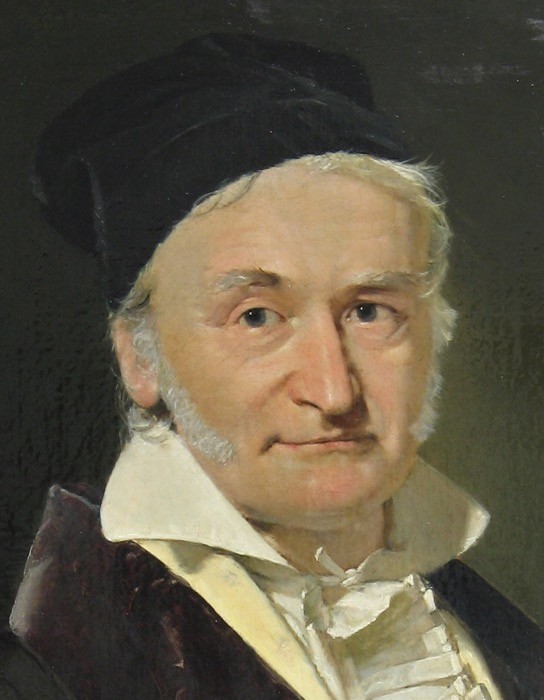
\includegraphics[height=0.35\textheight,keepaspectratio]{images/gauss_portrait.jpg}\\[2pt]
        {\scriptsize Carl Friedrich Gauß (1777--1855)\\
         G.\ Biermann nach C.\,A.\ Jensen, gemeinfrei\par}
      \end{center}
    \end{column}
    \begin{column}{0.72\textwidth}
      \small
      \begin{block}{Methode der kleinsten Quadrate (KQ-Methode)}
        Das klassische Verfahren, um die Parameter einer Geraden aus Daten
        zu bestimmen -- englisch \textbf{Ordinary Least Squares (OLS)}.
      \end{block}
      \begin{block}{Historische Einordnung}
        Gauß (Göttingen) nutzte die Methode nach eigener Angabe schon 1795.
        Zuerst \emph{veröffentlicht} hat sie Legendre (1805), Gauß erst 1809
        -- ein berühmter Prioritätsstreit.
      \end{block}
      \begin{exampleblock}{Grundgedanke}
        Miss, wie weit jede Beobachtung von der Geraden entfernt liegt, und
        wähle die Gerade, bei der diese Abstände \emph{insgesamt} am kleinsten
        sind. Die \glqq Quadrate\grqq{} im Namen: jetzt Schritt für Schritt.
      \end{exampleblock}
    \end{column}
  \end{columns}
\end{frame}

% ---- D1: Ein einzelnes Residuum ------------------------------
\begin{frame}{Nicht alle Punkte liegen auf der Geraden}
  \begin{columns}[T]
    \begin{column}{0.55\textwidth}
      \begin{tikzpicture}
        \begin{axis}[regplot, height=5.5cm, width=7.4cm, clip mode=individual]
          \werbepunkte
          \addplot[hsbiblue, thick, domain=0:14, samples=2] {30+1.2*x};
          \node[hsbiblue, font=\footnotesize\bfseries, anchor=west] at (axis cs:14.2,46.8) {D};
          % Residuum der Filiale 9
          \draw[resred, line width=1.6pt, visible on=<3->] (axis cs:10,45) -- (axis cs:10,42);
          \addplot[only marks, mark=*, mark size=3pt, hsbiaccent, visible on=<1->] coordinates {(10,45)};
          \node[hsbiaccent, font=\footnotesize, anchor=south east, fill=white, inner sep=1pt, xshift=-2pt, yshift=2pt, visible on=<1->] at (axis cs:9.8,45.9) {$y_9 = 45$};
          \addplot[only marks, mark=o, mark size=3pt, line width=1pt, hsbibluedark, visible on=<2->] coordinates {(10,42)};
          \node[hsbibluedark, font=\footnotesize, anchor=north west, fill=white, inner sep=1pt, xshift=2pt, yshift=-2pt, visible on=<2->] at (axis cs:10.2,39.6) {$\hat{y}_9 = 42$};
          \node[resred, font=\footnotesize, anchor=east, fill=white, inner sep=1pt, visible on=<3->] at (axis cs:9.6,44.8) {$\hat{u}_9 = 3$};
        \end{axis}
      \end{tikzpicture}
    \end{column}
    \begin{column}{0.44\textwidth}
      \small
      \begin{block}{Filiale 9: $x_9 = 10$}
        \begin{itemize}
          \item<1-> beobachtet: $y_9 = 45$
          \item<2-> auf der Geraden: $\hat{y}_9 = 30 + 1{,}2\cdot 10 = 42$
          \item<3-> Abstand: $45 - 42 = 3$
        \end{itemize}
      \end{block}
      \uncover<3->{\begin{block}{Residuum}
        \begin{center}
          $\hat{u}_i \;=\; y_i - \hat{y}_i$
        \end{center}
        \vspace{-4pt}
        Der \textbf{vertikale} Abstand zwischen Beobachtung und Gerade (nicht
        der kürzeste Abstand senkrecht zur Geraden). In Lehrbüchern auch $e_i$ statt $\hat{u}_i$.
      \end{block}}
    \end{column}
  \end{columns}
\end{frame}

% ---- D2: Alle Residuen ---------------------------------------
\begin{frame}{Die Residuen aller Beobachtungen}
  \begin{columns}[T]
    \begin{column}{0.55\textwidth}
      \begin{tikzpicture}
        \begin{axis}[regplot, height=5.5cm, width=7.4cm, clip mode=individual]
          \residuenvon{\werbelist}{30}{1.2}{resred, line width=1.6pt}
          \werbepunkte
          \addplot[hsbiblue, thick, domain=0:14, samples=2] {30+1.2*x};
          \node[hsbiblue, font=\footnotesize\bfseries, anchor=west] at (axis cs:14.2,46.8) {D};
        \end{axis}
      \end{tikzpicture}
    \end{column}
    \begin{column}{0.44\textwidth}
      \small
      \begin{block}{Vorzeichen der Residuen}
        \begin{itemize}
          \item Punkt \textbf{oberhalb} der Geraden: $y_i > \hat{y}_i$, also $\hat{u}_i > 0$
          \item Punkt \textbf{unterhalb}: $\hat{u}_i < 0$
          \item Punkt \textbf{auf} der Geraden: $\hat{u}_i = 0$
        \end{itemize}
        Gerade D: $1{,}8$; $-3{,}6$; $2{,}2$; $-3{,}0$; $0{,}8$; $1{,}4$; $-0{,}6$; $2{,}2$;
        $3{,}0$; $-3{,}2$; $-2{,}4$; $1{,}4$
      \end{block}
      \kernaussage{Gesucht ist die Gerade, bei der die Abweichungen zwischen
        beobachteten und angepassten Werten \emph{insgesamt} möglichst klein sind.}
    \end{column}
  \end{columns}
\end{frame}

% ---- D3a: Residuensumme --------------------------------------
\begin{frame}{Warum addieren wir nicht einfach die Residuen?}
  \begin{block}{Naheliegende Idee}
    \glqq Insgesamt klein\grqq{} könnte heißen: Die Summe der Residuen
    $\sum_{i=1}^{n} \hat{u}_i$ soll möglichst klein sein.
  \end{block}

  \begin{columns}[T]
    \begin{column}{0.5\textwidth}
      \begin{alertblock}{Das Problem}
        Positive und negative Residuen \textbf{heben sich auf}. Für Gerade D:
        $1{,}8 - 3{,}6 + 2{,}2 - 3{,}0 + \ldots + 1{,}4 = 0$.
        Die Summe ist null, obwohl kein Punkt auf der Geraden liegt.
      \end{alertblock}
    \end{column}
    \begin{column}{0.48\textwidth}
      \begin{exampleblock}{Bekannt von der Varianz}
        Abweichungen vom Mittelwert summieren sich stets zu null:
        $\sum_{i=1}^{n} (x_i - \bar{x}) = 0$.
        Beispiel: $2,\,4,\,9$ mit $\bar{x} = 5$, Abweichungen $-3,\,-1,\,+4$.
      \end{exampleblock}
    \end{column}
  \end{columns}

  \medskip
  Deshalb wurden bei der Varianz die Abweichungen \textbf{quadriert}.
  Zuvor prüfen wir: Gilt das Problem auch für andere Geraden?
\end{frame}

% ---- D3b: Residuensumme der vier Geraden ---------------------
\begin{frame}{Die Residuensumme unterscheidet gute und schlechte Geraden nicht}
  \begin{columns}[T]
    \begin{column}{0.46\textwidth}
      \begin{tikzpicture}
        \begin{axis}[regplot, height=4.5cm, width=6.4cm, clip mode=individual]
          \residuenvon{\werbelist}{24}{2}{resred, line width=1.4pt}
          \werbepunkte
          \addplot[hsbiaccent, thick, domain=0:14, samples=2] {24+2*x};
          \node[hsbiaccent, font=\footnotesize\bfseries, anchor=west] at (axis cs:14.2,52.5) {A};
        \end{axis}
      \end{tikzpicture}
      \begin{center}\footnotesize
        Gerade A: Residuen $7$, $0$, $5$, $-1$, $2$, $1$, $-1$, $1$, $1$, $-6$, $-6$, $-3$
        -- Summe $0$
      \end{center}
    \end{column}
    \begin{column}{0.52\textwidth}
      \small
      \begin{center}
        \renewcommand{\arraystretch}{1.05}
        \begin{tabular}{llr}
          \toprule
          Gerade & & $\sum \hat{u}_i$ \\
          \midrule
          A & zu steil   & $0$   \\
          B & zu flach   & $0$   \\
          C & zu hoch    & $-60$ \\
          D & passt gut  & $0$   \\
          \bottomrule
        \end{tabular}
      \end{center}
      \begin{alertblock}{Zwei Befunde}
        \begin{itemize}
          \item A, B und D: dieselbe Summe $0$, obwohl A und B schlecht passen.
          \item Je höher eine Gerade liegt, desto negativer die Summe:
                \glqq kleinste Summe\grqq{} wäre absurd.
        \end{itemize}
      \end{alertblock}
    \end{column}
  \end{columns}
\end{frame}

% ---- D4: Quadrieren ------------------------------------------
\begin{frame}{Die Lösung: Wir quadrieren die Abweichungen}
  \begin{block}{Quadrierte Residuen}
    \[
      \hat{u}_i^{\,2} \;=\; \bigl(y_i - \hat{y}_i\bigr)^{2}
    \]
  \end{block}

  \begin{center}
    \scriptsize
    \renewcommand{\arraystretch}{1.1}
    \begin{tabular}{l*{12}{r}r}
      \toprule
      Gerade D & 1 & 2 & 3 & 4 & 5 & 6 & 7 & 8 & 9 & 10 & 11 & 12 & Summe \\
      \midrule
      $\hat{u}_i$      & $1{,}8$  & $-3{,}6$  & $2{,}2$  & $-3{,}0$ & $0{,}8$  & $1{,}4$  & $-0{,}6$ & $2{,}2$  & $3{,}0$  & $-3{,}2$  & $-2{,}4$ & $1{,}4$  & $0$ \\
      $\hat{u}_i^{\,2}$ & $3{,}24$ & $12{,}96$ & $4{,}84$ & $9{,}00$ & $0{,}64$ & $1{,}96$ & $0{,}36$ & $4{,}84$ & $9{,}00$ & $10{,}24$ & $5{,}76$ & $1{,}96$ & $\mathbf{64{,}8}$ \\
      \bottomrule
    \end{tabular}
  \end{center}

  \begin{columns}[T]
    \begin{column}{0.55\textwidth}
      \begin{block}{Vorteile des Quadrierens}
        \begin{itemize}
          \item Alle Summanden sind $\ge 0$: Nichts hebt sich auf.
          \item Große Abweichungen zählen \emph{überproportional}:
                $3{,}6^{2} = 12{,}96$, aber $0{,}6^{2} = 0{,}36$.
          \item Die Summe lässt sich gut minimieren (Differentialrechnung).
        \end{itemize}
      \end{block}
    \end{column}
    \begin{column}{0.43\textwidth}
      \begin{exampleblock}{Derselbe Trick wie bei der Varianz}
        $s^{2} = \frac{1}{n-1}\sum (x_i - \bar{x})^{2}$ nutzt \emph{quadrierte}
        Abweichungen vom Mittel. Hier: quadrierte Abweichungen von einer
        \emph{Geraden}.
      \end{exampleblock}
    \end{column}
  \end{columns}
\end{frame}

% ---- D5a: Residuenquadrate als Flächen -----------------------
\begin{frame}{Quadrierte Residuen als Flächen}
  \begin{columns}[T]
    \begin{column}{0.36\textwidth}
      \begin{center}
      \begin{tikzpicture}
        \begin{axis}[regplot, scale only axis, height=4.8cm, width=3.27cm,
            xmin=0, xmax=15, ymin=28, ymax=50, xtick={0,5,10,15}, ytick={30,35,...,50}]
          \quadratevon{\werbelist}{30}{1.2}{draw=resred, fill=resred, fill opacity=0.2, line width=0.8pt}
          \residuenvon{\werbelist}{30}{1.2}{resred, line width=1.4pt}
          \werbepunkte
          \addplot[hsbiblue, thick, domain=0:15, samples=2] {30+1.2*x};
        \end{axis}
      \end{tikzpicture}
      \end{center}
    \end{column}
    \begin{column}{0.62\textwidth}
      \small
      \begin{block}{Konstruktion}
        \begin{itemize}
          \item Jedes rote Residuum wird zur Seite eines Quadrats:
                Seitenlänge $|\hat{u}_i|$, Fläche $\hat{u}_i^{\,2}$.
          \item Die Summe aller Flächen ist die Residuenquadratsumme,
                für Gerade D: $\sum \hat{u}_i^{\,2} = 64{,}8$.
        \end{itemize}
      \end{block}
      \kernaussage{Die beste Gerade ist diejenige, bei der die
        \textbf{Summe dieser Quadratflächen} möglichst klein ist.}
      \footnotesize Skalierung: Beide Achsen in Tsd.\ Euro, eine Einheit ist auf
      beiden Achsen gleich lang. Nur so sind die Quadrate wirklich Quadrate und
      ihre Flächen vergleichbar.
    \end{column}
  \end{columns}
\end{frame}

% ---- D5b: Vergleich schlecht vs. optimal ---------------------
\begin{frame}{Vergleich: schlecht passende Gerade und beste Gerade}
  \begin{columns}[T]
    \begin{column}{0.3\textwidth}
      \begin{center}
      \begin{tikzpicture}
        \begin{axis}[regplot, scale only axis, height=3.544cm, width=2.59cm,
            xlabel={$x$ (Tsd.\ Euro)}, ylabel={$y$ (Tsd.\ Euro)},
            xmin=0, xmax=19, ymin=25, ymax=51, xtick={0,5,10,15}, ytick={25,30,...,50}]
          \quadratevon{\werbelist}{24}{2}{draw=resred, fill=resred, fill opacity=0.2, line width=0.8pt}
          \residuenvon{\werbelist}{24}{2}{resred, line width=1.4pt}
          \werbepunkte
          \addplot[hsbiaccent, thick, domain=0:14, samples=2] {24+2*x};
        \end{axis}
      \end{tikzpicture}\\[1pt]
      {\footnotesize A: $\sum \hat{u}_i^{\,2} = \mathbf{164{,}0}$}
      \end{center}
    \end{column}
    \begin{column}{0.3\textwidth}
      \begin{center}
      \begin{tikzpicture}
        \begin{axis}[regplot, scale only axis, height=3.544cm, width=2.59cm,
            xlabel={$x$ (Tsd.\ Euro)}, ylabel={$y$ (Tsd.\ Euro)},
            xmin=0, xmax=19, ymin=25, ymax=51, xtick={0,5,10,15}, ytick={25,30,...,50}]
          \quadratevon{\werbelist}{30}{1.2}{draw=resred, fill=resred, fill opacity=0.2, line width=0.8pt}
          \residuenvon{\werbelist}{30}{1.2}{resred, line width=1.4pt}
          \werbepunkte
          \addplot[hsbiblue, thick, domain=0:14, samples=2] {30+1.2*x};
        \end{axis}
      \end{tikzpicture}\\[1pt]
      {\footnotesize D: $\sum \hat{u}_i^{\,2} = \mathbf{64{,}8}$}
      \end{center}
    \end{column}
    \begin{column}{0.37\textwidth}
      \small
      \begin{center}
        \renewcommand{\arraystretch}{1.0}
        \begin{tabular}{lr}
          \toprule
          Gerade & $\sum \hat{u}_i^{\,2}$ \\
          \midrule
          A & $164{,}0$ \\
          B & $120{,}6$ \\
          C & $364{,}8$ \\
          D & $\mathbf{64{,}8}$ \\
          \bottomrule
        \end{tabular}
      \end{center}
      \kernaussage{Die Quadratsumme trennt gute von schlechten Geraden.
        Gibt es eine noch bessere als D?}
      \appmarker{App 2: Quadrate und Summe live beim Verschieben.}
    \end{column}
  \end{columns}
\end{frame}

% ---- E1: Zielfunktion ----------------------------------------
\begin{frame}{Das Minimierungsproblem: Die Zielfunktion}
  \begin{block}{Residuenquadratsumme für beliebige Werte $\beta_0$ und $\beta_1$}
    \vspace{-2pt}
    \[
      S(\beta_0,\beta_1) \;=\; \sum_{i=1}^{n}\bigl(\,y_i - \beta_0 - \beta_1 x_i\,\bigr)^{2}
      \;=\; \sum_{i=1}^{n} \hat{u}_i^{\,2}
    \]
    $y_i$: beobachteter Wert; $\beta_0 + \beta_1 x_i$: Wert auf der Geraden bei
    $x_i$; Klammer: Residuum $\hat{u}_i$ dieser Geraden, quadriert und über alle
    $n$ Beobachtungen summiert.
  \end{block}

  \begin{block}{Gesucht: das Minimum}
    \vspace{-2pt}
    \[
      (\hat{\beta}_0,\hat{\beta}_1)
      \;=\;
      \underset{\beta_0,\,\beta_1}{\arg\min}\;
      \sum_{i=1}^{n}\bigl(y_i - \beta_0 - \beta_1 x_i\bigr)^{2}
    \]
    \textbf{In Worten:} die Parameterwerte mit der kleinsten Residuenquadratsumme.
    Beispiel: $S(24;\,2) = 164{,}0$ (A), $S(30;\,1{,}2) = 64{,}8$ (D).
  \end{block}
\end{frame}

% ---- E2: Lösungsweg ------------------------------------------
\begin{frame}{Wie lässt sich das Problem lösen?}
  \begin{columns}[T]
    \begin{column}{0.4\textwidth}
      \begin{tikzpicture}[font=\footnotesize]
        \begin{axis}[regbasis, height=4.8cm, width=5.8cm,
            xlabel={Parameter $\beta$}, ylabel={$S(\beta)$},
            xmin=-0.5, xmax=4.5, ymin=-1.6, ymax=10, xtick=\empty, ytick=\empty,
            grid=none]
          \addplot[hsbiblue, thick, domain=-0.3:4.3, samples=60] {1.2 + 1.6*(x-2)^2};
          \addplot[only marks, mark=*, mark size=2.6pt, resred] coordinates {(2,1.2)};
          \draw[resred, thick] (axis cs:1.2,1.2) -- (axis cs:2.8,1.2);
          \node[resred, anchor=north] at (axis cs:2,1.0) {Steigung $0$};
          \node[anchor=south, hsbibluedark] at (axis cs:2,2.1) {$\hat{\beta}$};
        \end{axis}
      \end{tikzpicture}
      \begin{center}\footnotesize
        Schema: nach oben geöffnete Parabel, im Minimum ist die Ableitung null.
      \end{center}
    \end{column}
    \begin{column}{0.58\textwidth}
      \begin{block}{Beobachtung}
        $S(\beta_0,\beta_1)$ ist eine \textbf{quadratische Funktion} der beiden
        Unbekannten: eine nach oben geöffnete \glqq Schüssel\grqq{} mit genau
        einem Minimum (sofern die $x_i$ nicht alle gleich sind).
      \end{block}
      \begin{block}{Lösungsweg mit Differentialrechnung}
        \begin{enumerate}
          \item $S$ nach $\beta_0$ ableiten.
          \item $S$ nach $\beta_1$ ableiten.
          \item Beide partiellen Ableitungen gleich null setzen.
          \item Das entstehende Gleichungssystem lösen.
        \end{enumerate}
      \end{block}
    \end{column}
  \end{columns}
\end{frame}

% ---- E2b: Bedingungen erster Ordnung -------------------------
\begin{frame}{Bedingungen erster Ordnung}
  \begin{block}{Ableiten mit der Kettenregel}
    Für einen einzelnen Summanden gilt
    $\frac{\partial}{\partial \beta_0}\bigl(y_i - \beta_0 - \beta_1 x_i\bigr)^{2}
      = 2\bigl(y_i - \beta_0 - \beta_1 x_i\bigr)\cdot(-1)$;
    bei $\beta_1$ lautet die innere Ableitung $-x_i$.
  \end{block}

  \begin{block}{Summieren und gleich null setzen}
    \vspace{-8pt}
    \begin{align*}
      \frac{\partial S}{\partial \beta_0} &= -2\sum_{i=1}^{n}\bigl(y_i - \beta_0 - \beta_1 x_i\bigr) \;=\; 0 \\
      \frac{\partial S}{\partial \beta_1} &= -2\sum_{i=1}^{n} x_i\bigl(y_i - \beta_0 - \beta_1 x_i\bigr) \;=\; 0
    \end{align*}
  \end{block}

  \textbf{In Worten:} Im Minimum verschwinden beide partiellen Ableitungen.
  Die Klammern sind die Residuen: Die beste Gerade hat die Residuensumme null
  und zusätzlich $\sum x_i \hat{u}_i = 0$.
\end{frame}

% ---- E3a: Normalgleichungen ----------------------------------
\begin{frame}{Von den Ableitungen zu den Normalgleichungen}
  \begin{block}{Erste Bedingung: durch $-2$ teilen, Summe aufspalten}
    \[
      \sum_{i=1}^{n} y_i \;=\; n\,\beta_0 + \beta_1 \sum_{i=1}^{n} x_i
      \qquad\Longrightarrow\qquad
      \beta_0 \;=\; \bar{y} - \beta_1\,\bar{x}
    \]
    \footnotesize (beide Seiten durch $n$ geteilt; $\bar{x} = \frac{1}{n}\sum x_i$, $\bar{y} = \frac{1}{n}\sum y_i$)
  \end{block}

  \begin{block}{Zweite Bedingung: ebenso}
    \[
      \sum_{i=1}^{n} x_i y_i \;=\; \beta_0 \sum_{i=1}^{n} x_i + \beta_1 \sum_{i=1}^{n} x_i^{2}
    \]
  \end{block}

  \begin{exampleblock}{Normalgleichungen}
    Zwei lineare Gleichungen für die zwei Unbekannten $\beta_0$ und $\beta_1$.
    Die erste liefert den Achsenabschnitt, sobald die Steigung bekannt ist.
  \end{exampleblock}
\end{frame}

% ---- E3b: Auflösen nach beta1 --------------------------------
\begin{frame}{Auflösen nach der Steigung}
  \begin{block}{Achsenabschnitt einsetzen}
    $\beta_0 = \bar{y} - \beta_1 \bar{x}$ in die zweite Normalgleichung einsetzen
    und $\sum x_i = n\bar{x}$ nutzen:
    \begin{align*}
      \sum x_i y_i &= (\bar{y} - \beta_1 \bar{x})\, n\bar{x} + \beta_1 \sum x_i^{2} \\
      \sum x_i y_i - n\,\bar{x}\bar{y} &= \beta_1 \Bigl(\sum x_i^{2} - n\,\bar{x}^{2}\Bigr)
    \end{align*}
  \end{block}

  \begin{block}{Ergebnis}
    Mit $\sum x_i y_i - n\bar{x}\bar{y} = \sum (x_i - \bar{x})(y_i - \bar{y})$ und
    $\sum x_i^{2} - n\bar{x}^{2} = \sum (x_i - \bar{x})^{2}$ folgt
    \[
      \hat{\beta}_1 \;=\; \frac{\sum_{i=1}^{n} (x_i - \bar{x})(y_i - \bar{y})}
                              {\sum_{i=1}^{n} (x_i - \bar{x})^{2}}
      \qquad\text{und}\qquad
      \hat{\beta}_0 \;=\; \bar{y} - \hat{\beta}_1\,\bar{x}.
    \]
  \end{block}

  \footnotesize Voraussetzung: Die $x_i$ sind nicht alle gleich (sonst Nenner null).
  Da $S$ nach oben geöffnet ist, liegt hier tatsächlich das Minimum.
\end{frame}

% ---- (KQ-Schätzer: weiterhin Subsection "Kleinste Quadrate") ----

% ---- F1: Schätzer für die Steigung ---------------------------
\begin{frame}{Der KQ-Schätzer für die Steigung}
  \begin{block}{Lösung des Minimierungsproblems}
    \[
      \hat{\beta}_1
      \;=\;
      \frac{\sum_{i=1}^{n} (x_i - \bar{x})(y_i - \bar{y})}
           {\sum_{i=1}^{n} (x_i - \bar{x})^{2}}
    \]
  \end{block}

  \begin{columns}[T]
    \begin{column}{0.5\textwidth}
      \begin{block}{Zähler}
        Produkte der Abweichungen vom jeweiligen Mittelwert, aufsummiert.
        \begin{itemize}
          \item beide über oder beide unter dem Mittel: Produkt $> 0$
          \item eines über, eines unter dem Mittel: Produkt $< 0$
        \end{itemize}
        Positiv, wenn die Punktwolke ansteigt.
      \end{block}
    \end{column}
    \begin{column}{0.48\textwidth}
      \begin{block}{Nenner}
        Quadrierte Abweichungen der $x_i$ vom Mittel, aufsummiert.
        \begin{itemize}
          \item stets $> 0$ (wenn die $x_i$ nicht alle gleich sind)
          \item misst die Streuung der erklärenden Variable
        \end{itemize}
      \end{block}
      \footnotesize Kommen Ihnen Zähler und Nenner bekannt vor?
    \end{column}
  \end{columns}
\end{frame}

% ---- F2a: Verbindung zu Kovarianz und Varianz ----------------
\begin{frame}{Die Verbindung zu Kovarianz und Varianz}
  \begin{columns}[T]
    \begin{column}{0.49\textwidth}
      \begin{block}{Empirische Kovarianz}
        \[
          s_{xy} \;=\; {\color{hsbiaccent}\frac{1}{n-1}}
          \sum_{i=1}^{n} (x_i - \bar{x})(y_i - \bar{y})
        \]
      \end{block}
    \end{column}
    \begin{column}{0.49\textwidth}
      \begin{block}{Empirische Varianz von $x$}
        \[
          s_x^{2} \;=\; {\color{hsbiaccent}\frac{1}{n-1}}
          \sum_{i=1}^{n} (x_i - \bar{x})^{2}
        \]
      \end{block}
    \end{column}
  \end{columns}

  \begin{block}{Der Schätzer, mit $\frac{1}{n-1}$ erweitert}
    \[
      \hat{\beta}_1
      \;=\;
      \frac{{\color{hsbiaccent}\frac{1}{n-1}}\sum_{i=1}^{n}(x_i-\bar{x})(y_i-\bar{y})}
           {{\color{hsbiaccent}\frac{1}{n-1}}\sum_{i=1}^{n}(x_i-\bar{x})^{2}}
      \;=\;
      \frac{s_{xy}}{s_x^{2}}
    \]
    Der Faktor ${\color{hsbiaccent}\frac{1}{n-1}}$ steht in Zähler \emph{und}
    Nenner und kürzt sich heraus. Was bleibt, sind zwei bekannte Kennzahlen.
  \end{block}
  \vspace{-8pt}
  \begin{center}
    \fbox{\rule[-6pt]{0pt}{20pt}\quad$\displaystyle \hat{\beta}_1 = \frac{s_{xy}}{s_x^{2}}$\quad}
  \end{center}
\end{frame}

% ---- F2b: Intuition und Beispiel -----------------------------
\begin{frame}{Steigung $=$ Kovarianz durch Varianz}
  \kernaussage{Die Steigung der Regressionsgeraden lässt sich unmittelbar aus
    zwei bereits bekannten Kennzahlen bestimmen: der \textbf{Kovarianz} von $x$
    und $y$ und der \textbf{Varianz} von $x$.}

  \begin{columns}[T]
    \begin{column}{0.5\textwidth}
      \begin{block}{Intuition}
        \begin{itemize}
          \item $s_{xy}$ beschreibt die \emph{gemeinsame} Variation von $x$ und $y$:
                Vorzeichen $=$ Richtung des Zusammenhangs.
          \item $s_x^{2}$ berücksichtigt, wie stark $x$ selbst streut.
          \item Ihr Verhältnis: Wie viel Mitbewegung von $y$ entfällt auf
                eine Einheit Streuung von $x$? Das ist die Steigung.
        \end{itemize}
      \end{block}
    \end{column}
    \begin{column}{0.48\textwidth}
      \mindestzeilenabstand
      \begin{exampleblock}{Zwölf Filialen}
        $\sum (x_i-\bar{x})(y_i-\bar{y}) = 186$, \quad
        $\sum (x_i-\bar{x})^{2} = 155$ \\[3pt]
        $\hat{\beta}_1 = 186/155 = 1{,}2$ \\[3pt]
        Über die Kennzahlen: $s_{xy} = 186/11 = 16{,}91$,
        $s_x^{2} = 155/11 = 14{,}09$ und damit ebenfalls
        $\hat{\beta}_1 = 16{,}91/14{,}09 = 1{,}2$.
      \end{exampleblock}
      \footnotesize Für die Steigung genügen die reinen Summen.
    \end{column}
  \end{columns}
\end{frame}

% ---- F3: Achsenabschnitt und Schwerpunkt ----------------------
\begin{frame}{Der KQ-Schätzer für den Achsenabschnitt}
  \begin{columns}[T]
    \begin{column}{0.5\textwidth}
      \begin{tikzpicture}
        \begin{axis}[regplot, height=5.4cm, width=7.4cm, yticklabel shift=2pt]
          \werbepunkte
          \addplot[hsbiblue, thick, domain=0:14, samples=2] {30+1.2*x};
          \draw[hsbigray, dashed] (axis cs:7.5,24) -- (axis cs:7.5,39) -- (axis cs:0,39);
          \addplot[only marks, mark=square*, mark size=3pt, hsbiaccent] coordinates {(7.5,39)};
          \node[hsbiaccent, font=\footnotesize, anchor=north west, fill=white, inner sep=1pt, xshift=2pt, yshift=-2pt] at (axis cs:7.7,38.6) {$(\bar{x},\bar{y}) = (7{,}5;\,39)$};
          \addplot[only marks, mark=*, mark size=2.6pt, hsbiaccent] coordinates {(0,30)};
          \node[hsbiaccent, font=\footnotesize, anchor=west, fill=white, inner sep=1pt, xshift=2pt] at (axis cs:0.3,27.6) {$\hat{\beta}_0 = 30$};
          \node[hsbigray, font=\footnotesize, anchor=south west, fill=white, inner sep=1pt, xshift=2pt, yshift=2pt] at (axis cs:7.7,24.2) {$\bar{x}$};
          \node[hsbigray, font=\footnotesize, anchor=west, fill=white, inner sep=1pt, xshift=2pt, yshift=1pt] at (axis cs:0.3,40.2) {$\bar{y}$};
        \end{axis}
      \end{tikzpicture}
    \end{column}
    \begin{column}{0.48\textwidth}
      \small
      \begin{block}{Aus der ersten Normalgleichung}
        \vspace{-4pt}
        \[
          \hat{\beta}_0 \;=\; \bar{y} - \hat{\beta}_1\,\bar{x}
          \quad\Longleftrightarrow\quad
          \bar{y} = \hat{\beta}_0 + \hat{\beta}_1 \bar{x}
        \]
        Der Punkt $(\bar{x},\bar{y})$ liegt \textbf{auf} der KQ-Geraden.
      \end{block}
      \begin{exampleblock}{Schwerpunkt der Punktwolke}
        Die KQ-Gerade verläuft stets durch den Schwerpunkt $(\bar{x},\bar{y})$;
        mit der Steigung ist sie damit festgelegt.
        Beispiel: $\hat{\beta}_0 = 39 - 1{,}2 \cdot 7{,}5 = 30$.
      \end{exampleblock}
      \footnotesize Rückblick: Jede Gerade durch $(\bar{x},\bar{y})$ hat die
      Residuensumme $0$, auch A und B. Das erklärt die Tabelle von vorhin.
    \end{column}
  \end{columns}
\end{frame}

% ---- F4: Beide Schätzer im Überblick --------------------------
\begin{frame}{Beide Schätzer im Überblick}
  \begin{block}{Die Lösung des Minimierungsproblems}
    \[
      \hat{\beta}_1 \;=\; \frac{s_{xy}}{s_x^{2}}
      \qquad\qquad
      \hat{\beta}_0 \;=\; \bar{y} - \hat{\beta}_1\,\bar{x}
    \]
  \end{block}

  \begin{block}{Die geschätzte Regressionsgerade}
    \[
      \hat{y}_i \;=\; \hat{\beta}_0 + \hat{\beta}_1\, x_i
      \qquad\text{für die zwölf Filialen:}\quad \hat{y}_i = 30 + 1{,}2\,x_i
    \]
    Gerade D \emph{war} die KQ-Gerade: Keine andere hat eine kleinere
    Residuenquadratsumme als $64{,}8$.
  \end{block}

  \kernaussage{Das Ausgangsproblem ist gelöst: Aus $\bar{x}$, $\bar{y}$, $s_{xy}$
    und $s_x^{2}$ erhalten wir die eindeutig beste Gerade -- beste im Sinne der
    kleinsten Residuenquadratsumme.}

  \footnotesize Die Steigung hat stets das Vorzeichen der Kovarianz; für
  $s_{xy} = 0$ ist die Gerade waagerecht.
\end{frame}

% ---- G: Schritt-für-Schritt ----------------------------------
\begin{frame}{Schritt für Schritt zur Regressionsgeraden}
  \begin{columns}[T]
    \begin{column}{0.4\textwidth}
      \begin{block}{Rechenschema}
        \small
        \begin{enumerate}
          \setlength{\itemsep}{1pt}
          \item Mittelwerte $\bar{x}$, $\bar{y}$
          \item Kovarianz $s_{xy} = \frac{1}{n-1}\sum (x_i-\bar{x})(y_i-\bar{y})$
          \item Varianz $s_x^{2} = \frac{1}{n-1}\sum (x_i-\bar{x})^{2}$
          \item Steigung $\hat{\beta}_1 = s_{xy} / s_x^{2}$
          \item Achsenabschnitt $\hat{\beta}_0 = \bar{y} - \hat{\beta}_1 \bar{x}$
          \item Gerade $\hat{y} = \hat{\beta}_0 + \hat{\beta}_1 x$
        \end{enumerate}
      \end{block}
      \footnotesize Die Mittelwerte zuerst: Alle weiteren Schritte benötigen sie.
    \end{column}
    \begin{column}{0.58\textwidth}
      \begin{block}{Arbeitstabelle für die Schritte 2 und 3}
        \begin{center}
          \scriptsize
          \renewcommand{\arraystretch}{1.2}
          \setlength{\tabcolsep}{3pt}
          \begin{tabular}{c|cc|cc|cc}
            \toprule
            $i$ & $x_i$ & $y_i$ & $x_i-\bar{x}$ & $y_i-\bar{y}$ & $(x_i-\bar{x})(y_i-\bar{y})$ & $(x_i-\bar{x})^{2}$ \\
            \midrule
            1 & & & & & & \\
            2 & & & & & & \\
            $\vdots$ & & & & & & \\
            $n$ & & & & & & \\
            \midrule
            $\sum$ & & & $0$ & $0$ & $\to s_{xy}$ & $\to s_x^{2}$ \\
            \bottomrule
          \end{tabular}
        \end{center}
        \small Kontrolle: Die Spalten $x_i-\bar{x}$ und $y_i-\bar{y}$ summieren
        sich zu~$0$.
      \end{block}
    \end{column}
  \end{columns}
\end{frame}

% ---- H: Übungsaufgabe ----------------------------------------
\begin{frame}{Übungsaufgabe: Eine Regressionsgerade selbst bestimmen}
  \begin{block}{Daten}
    Werbeaufwand und Umsatz eines Online-Shops in fünf Monaten (jeweils in Tsd.\ Euro):
    \begin{center}
      \renewcommand{\arraystretch}{1.05}
      \begin{tabular}{l*{5}{r}}
        \toprule
        Monat $i$                       & 1  & 2  & 3  & 4  & 5  \\
        \midrule
        Werbeaufwand $x_i$ (Tsd.\ Euro) & 1  & 2  & 3  & 4  & 5  \\
        Umsatz $y_i$ (Tsd.\ Euro)       & 21 & 26 & 24 & 30 & 29 \\
        \bottomrule
      \end{tabular}
    \end{center}
  \end{block}

  \begin{exampleblock}{Aufgaben}
    \begin{columns}[T]
      \begin{column}{0.47\textwidth}
        \begin{enumerate}[a)]
          \item Mittelwerte beider Variablen berechnen.
          \item Empirische Kovarianz $s_{xy}$ berechnen.
          \item Empirische Varianz $s_x^{2}$ berechnen.
        \end{enumerate}
      \end{column}
      \begin{column}{0.51\textwidth}
        \begin{enumerate}[a)]
          \setcounter{enumi}{3}
          \item KQ-Schätzer für die Steigung bestimmen.
          \item KQ-Schätzer für den Achsenabschnitt bestimmen.
          \item Geschätzte Regressionsgerade angeben.
        \end{enumerate}
      \end{column}
    \end{columns}
  \end{exampleblock}
\end{frame}

% ---- H Lösung 1 ----------------------------------------------
\begin{frame}{Lösung (1/3): Mittelwerte und Arbeitstabelle}
  \begin{block}{a) Mittelwerte}
    \[
      \bar{x} = \frac{1+2+3+4+5}{5} = \frac{15}{5} = 3
      \qquad\qquad
      \bar{y} = \frac{21+26+24+30+29}{5} = \frac{130}{5} = 26
    \]
    \vspace{-10pt}
  \end{block}

  \begin{block}{Arbeitstabelle}
    \begin{center}
      \renewcommand{\arraystretch}{1.0}
      \begin{tabular}{c|cc|cc|cc}
        \toprule
        $i$ & $x_i$ & $y_i$ & $x_i-\bar{x}$ & $y_i-\bar{y}$ & $(x_i-\bar{x})(y_i-\bar{y})$ & $(x_i-\bar{x})^{2}$ \\
        \midrule
        1 & 1 & 21 & $-2$ & $-5$ & $10$ & $4$ \\
        2 & 2 & 26 & $-1$ & $0$  & $0$  & $1$ \\
        3 & 3 & 24 & $0$  & $-2$ & $0$  & $0$ \\
        4 & 4 & 30 & $1$  & $4$  & $4$  & $1$ \\
        5 & 5 & 29 & $2$  & $3$  & $6$  & $4$ \\
        \midrule
        $\sum$ & 15 & 130 & $0$ & $0$ & $\mathbf{20}$ & $\mathbf{10}$ \\
        \bottomrule
      \end{tabular}
    \end{center}
  \end{block}
\end{frame}

% ---- H Lösung 2 ----------------------------------------------
\begin{frame}{Lösung (2/3): Kovarianz, Varianz und Schätzer}
  \begin{columns}[T]
    \begin{column}{0.49\textwidth}
      \begin{block}{b) Kovarianz}
        \[
          s_{xy} = \frac{1}{n-1}\sum (x_i-\bar{x})(y_i-\bar{y}) = \frac{20}{4} = \mathbf{5}
        \]
      \end{block}
      \begin{block}{c) Varianz von $x$}
        \[
          s_x^{2} = \frac{1}{n-1}\sum (x_i-\bar{x})^{2} = \frac{10}{4} = \mathbf{2{,}5}
        \]
      \end{block}
    \end{column}
    \begin{column}{0.49\textwidth}
      \begin{block}{d) Steigung}
        \[
          \hat{\beta}_1 = \frac{s_{xy}}{s_x^{2}} = \frac{5}{2{,}5} = \mathbf{2}
        \]
        Kontrolle über die Summen: $20/10 = 2$.
      \end{block}
      \begin{block}{e) Achsenabschnitt}
        \[
          \hat{\beta}_0 = \bar{y} - \hat{\beta}_1\,\bar{x} = 26 - 2\cdot 3 = \mathbf{20}
        \]
      \end{block}
    \end{column}
  \end{columns}

  \begin{exampleblock}{f) Geschätzte Regressionsgerade}
    \[
      \hat{y} \;=\; 20 + 2\,x
    \]
    Einheiten: $\hat{\beta}_1 = 2$ Tsd.\ Euro Umsatz je Tsd.\ Euro Werbeaufwand;
    $\hat{\beta}_0 = 20$ Tsd.\ Euro.
  \end{exampleblock}
\end{frame}

% ---- H Lösung 3 ----------------------------------------------
\begin{frame}{Lösung (3/3): Die Gerade im Streuungsdiagramm}
  \begin{columns}[T]
    \begin{column}{0.52\textwidth}
      \begin{tikzpicture}
        \begin{axis}[uebplot, height=5.6cm, width=7.6cm]
          \residuenvon{\uebliste}{20}{2}{resred, line width=1.4pt}
          \uebpunkte
          \addplot[hsbiblue, thick, domain=0:6, samples=2] {20+2*x};
          \addplot[only marks, mark=square*, mark size=3pt, hsbiaccent] coordinates {(3,26)};
          \node[hsbiaccent, font=\footnotesize, anchor=north west, fill=white, inner sep=1pt, xshift=2pt, yshift=-2pt] at (axis cs:3.1,25.6) {$(\bar{x},\bar{y})$};
          \node[hsbiblue, font=\footnotesize, anchor=south east, xshift=-1.5pt] at (axis cs:5.9,31.5) {$\hat{y} = 20 + 2x$};
        \end{axis}
      \end{tikzpicture}
    \end{column}
    \begin{column}{0.46\textwidth}
      \begin{block}{Kontrolle}
        \begin{itemize}
          \item Die Gerade verläuft durch den Schwerpunkt $(3;\,26)$.
          \item Residuen $\hat{u}_i = y_i - \hat{y}_i$:
                $-1,\ 2,\ -2,\ 2,\ -1$ -- Summe $0$.
          \item Residuenquadratsumme: $1 + 4 + 4 + 4 + 1 = 14$.
        \end{itemize}
      \end{block}
      \begin{exampleblock}{Probe mit anderen Geraden}
        $\hat{y} = 19 + 2x$: Residuen $0, 3, -1, 3, 0$, Quadratsumme $19 > 14$.
        $\hat{y} = 20 + 2{,}5x$: Quadratsumme $27{,}75 > 14$.
      \end{exampleblock}
    \end{column}
  \end{columns}
\end{frame}

% ===== SUBSECTION: INTERPRETATION =====
\subsection{Interpretation}

% ---- I1: Steigung ---------------------------------------------
\begin{frame}{Wie interpretieren wir die Steigung?}
  \begin{columns}[T]
    \begin{column}{0.5\textwidth}
      \begin{tikzpicture}
        \begin{axis}[uebplot, height=5.4cm, width=7.4cm]
          \uebpunkte
          \addplot[hsbiblue, thick, domain=0:6, samples=2] {20+2*x};
          \draw[hsbigray, dashed] (axis cs:2,16) -- (axis cs:2,24) -- (axis cs:0,24);
          \draw[hsbigray, dashed] (axis cs:3,16) -- (axis cs:3,26) -- (axis cs:0,26);
          \draw[hsbigreen, very thick] (axis cs:2,24) -- (axis cs:3,24) -- (axis cs:3,26);
          \node[hsbigreen, font=\footnotesize, below] at (axis cs:2.5,24) {$+1$};
          \node[hsbigreen, font=\footnotesize, right] at (axis cs:3,25.4) {$+2 = \hat{\beta}_1$};
          \addplot[only marks, mark=o, mark size=2.6pt, line width=1pt, hsbibluedark] coordinates {(2,24) (3,26)};
        \end{axis}
      \end{tikzpicture}
    \end{column}
    \begin{column}{0.48\textwidth}
      \small
      \begin{block}{Steigung $\hat{\beta}_1 = 2$}
        Steigt $x$ um eine Einheit, so ändert sich der durch die Gerade
        beschriebene Wert von $y$ um $\hat{\beta}_1$ Einheiten. Hier:
        Werbeaufwand $2 \to 3$ Tsd.\ Euro, $\hat{y}$ steigt von $24$ auf $26$.
        \textbf{Je zusätzlichem Tsd.\ Euro Werbeaufwand ist laut Gerade ein um
        $2$ Tsd.\ Euro höherer Umsatz zu erwarten.}
      \end{block}
      \begin{alertblock}{Keine kausale Aussage}
        Die Gerade beschreibt einen statistischen Zusammenhang. Dass mehr
        Werbung den Umsatz \emph{verursacht}, folgt daraus nicht -- etwa, wenn
        in umsatzstarken Monaten ohnehin mehr geworben wird.
      \end{alertblock}
    \end{column}
  \end{columns}
\end{frame}

% ---- I2: Achsenabschnitt --------------------------------------
\begin{frame}{Wie interpretieren wir den Achsenabschnitt?}
  \begin{columns}[T]
    \begin{column}{0.5\textwidth}
      \begin{tikzpicture}
        \begin{axis}[uebplot, height=5.4cm, width=7.4cm, yticklabel shift=2pt]
          \uebpunkte
          \addplot[hsbiblue, thick, domain=0:6, samples=2] {20+2*x};
          \addplot[only marks, mark=*, mark size=3pt, hsbiaccent] coordinates {(0,20)};
          \draw[hsbigray, dashed] (axis cs:1,16) -- (axis cs:1,34);
          \draw[hsbigray, dashed] (axis cs:5,16) -- (axis cs:5,34);
          \node[hsbiaccent, font=\footnotesize, anchor=west, fill=white, inner sep=1pt] at (axis cs:0.2,18.8) {$\hat{\beta}_0 = 20$};
          \draw[hsbigray, <->, >=Latex] (axis cs:1,31.6) -- (axis cs:5,31.6);
          \node[hsbigray, font=\footnotesize, anchor=south, fill=white, inner sep=1pt] at (axis cs:3,31.7) {beobachteter Bereich};
        \end{axis}
      \end{tikzpicture}
    \end{column}
    \begin{column}{0.48\textwidth}
      \small\mindestzeilenabstand
      \begin{block}{Achsenabschnitt $\hat{\beta}_0 = 20$}
        $\hat{\beta}_0 = \hat{y}\,\big|_{x=0}$: der Wert der Geraden bei $x = 0$.
        Hier: laut Gerade $20$ Tsd.\ Euro Umsatz in einem Monat ohne Werbung.
      \end{block}
      \begin{alertblock}{Vorsicht bei der Deutung}
        \begin{itemize}
          \item $x = 0$ wurde \emph{nicht beobachtet} (Daten: $1$ bis $5$):
                Die Gerade wird dorthin \emph{extrapoliert}.
          \item Liegt $x = 0$ weit außerhalb des Datenbereichs, hat
                $\hat{\beta}_0$ oft keine inhaltliche Bedeutung; er legt dann
                nur die Höhe der Geraden fest.
        \end{itemize}
      \end{alertblock}
    \end{column}
  \end{columns}
\end{frame}

% ---- I3: Zusammenfassung und Aufgabe --------------------------
\begin{frame}{Interpretation im Überblick}
  \begin{columns}[T]
    \begin{column}{0.46\textwidth}
      \begin{tikzpicture}
        \begin{axis}[uebplot, height=5.4cm, width=6.8cm, yticklabel shift=2pt]
          \uebpunkte
          \addplot[hsbiblue, thick, domain=0:6, samples=2] {20+2*x};
          \addplot[only marks, mark=*, mark size=3pt, hsbiaccent] coordinates {(0,20)};
          \node[hsbiaccent, font=\footnotesize, anchor=west, fill=white, inner sep=1pt, xshift=2pt] at (axis cs:0.2,18.8) {$\hat{\beta}_0 = 20$};
          \draw[hsbigreen, very thick] (axis cs:2,24) -- (axis cs:3,24) -- (axis cs:3,26);
          \node[hsbigreen, font=\footnotesize, right] at (axis cs:3,25.4) {$\hat{\beta}_1 = 2$};
          \node[hsbiblue, font=\footnotesize, anchor=south east] at (axis cs:5.9,31.5) {$\hat{y} = 20 + 2x$};
        \end{axis}
      \end{tikzpicture}
    \end{column}
    \begin{column}{0.52\textwidth}
      \small
      \begin{block}{$\hat{y} = {\color{hsbiaccent}\hat{\beta}_0} + {\color{hsbigreen}\hat{\beta}_1}\,x = {\color{hsbiaccent}20} + {\color{hsbigreen}2}\,x$}
        \begin{description}
          \item[{\color{hsbiaccent}$\hat{\beta}_0 = 20$}] Höhe der Geraden bei $x = 0$:
                Umsatz laut Gerade ohne Werbung (Extrapolation).
          \item[{\color{hsbigreen}$\hat{\beta}_1 = 2$}] Je Tsd.\ Euro mehr Werbung
                $2$ Tsd.\ Euro mehr Umsatz laut Gerade; kein Kausalbeweis.
        \end{description}
      \end{block}
      \begin{exampleblock}{Aufgabe}
        Für ein anderes Unternehmen wurde $\hat{y} = 12 + 0{,}8\,x$ geschätzt
        (gleiche Variablen und Einheiten, beobachtet: $x$ von $5$ bis $40$).
        Erläutern Sie beide Parameter in eigenen Worten.
      \end{exampleblock}
    \end{column}
  \end{columns}
\end{frame}

% ---- Leuchte 1: Berechnung ------------------------------------
\begin{frame}{Zweites Beispiel: Preis und Absatz der Leuchte}
  \begin{block}{Daten aus dem Einstieg ($n = 9$ Geschäfte) und Arbeitstabelle}
    \begin{center}
      \scriptsize
      \renewcommand{\arraystretch}{1.05}
      \begin{tabular}{l*{9}{r}r}
        \toprule
        Preis $x_i$ (Euro)          & 80   & 85   & 90   & 95   & 100 & 105  & 110  & 115  & 120  & $\sum$ \\
        Menge $y_i$                 & 20   & 17   & 15   & 9    & 11  & 8    & 4    & 4    & 2    & \\
        \midrule
        $x_i - \bar{x}$             & $-20$ & $-15$ & $-10$ & $-5$ & $0$ & $5$ & $10$ & $15$ & $20$ & $0$ \\
        $y_i - \bar{y}$             & $10$ & $7$  & $5$  & $-1$ & $1$ & $-2$ & $-6$ & $-6$ & $-8$ & $0$ \\
        $(x_i-\bar{x})(y_i-\bar{y})$ & $-200$ & $-105$ & $-50$ & $-5$ & $0$ & $-10$ & $-60$ & $-90$ & $-160$ & $\mathbf{-670}$ \\
        $(x_i-\bar{x})^{2}$         & $400$ & $225$ & $100$ & $25$ & $0$ & $25$ & $100$ & $225$ & $400$ & $\mathbf{1500}$ \\
        \bottomrule
      \end{tabular}
    \end{center}
  \end{block}

  \begin{columns}[T]
    \begin{column}{0.5\textwidth}
      \begin{block}{Schritte 1 bis 3}
        \small
        $\bar{x} = 900/9 = 100$, \quad $\bar{y} = 90/9 = 10$ \\
        $s_{xy} = -670/8 = -83{,}75$, \quad $s_x^{2} = 1500/8 = 187{,}5$
      \end{block}
    \end{column}
    \begin{column}{0.48\textwidth}
      \begin{block}{Schritte 4 bis 6}
        \small
        $\hat{\beta}_1 = -83{,}75 / 187{,}5 = -0{,}4467$ \\
        $\hat{\beta}_0 = 10 - (-0{,}4467)\cdot 100 = 54{,}67$ \\
        $\hat{y} = 54{,}67 - 0{,}4467\,x$
      \end{block}
    \end{column}
  \end{columns}
\end{frame}

% ---- Leuchte 2: Grafik und Interpretation --------------------
\begin{frame}{Preis und Absatz: Interpretation der Koeffizienten}
  \begin{columns}[T]
    \begin{column}{0.5\textwidth}
      \begin{tikzpicture}
        \begin{axis}[leuchteplot, height=5.6cm, width=7.4cm]
          \residuenvon{\leuchteliste}{54.6667}{-0.44667}{resred, line width=1.2pt}
          \leuchtepunkte
          \addplot[hsbiblue, thick, domain=75:125, samples=2] {54.6667-0.44667*x};
        \end{axis}
      \end{tikzpicture}
    \end{column}
    \begin{column}{0.48\textwidth}
      \small
      \begin{block}{Steigung $\hat{\beta}_1 = -0{,}4467$}
        Steigt der Preis um $1$ Euro, so sinkt die laut Gerade erwartete
        Absatzmenge um $0{,}4467$ Stück: eine fallende
        \textbf{Preis-Absatz-Funktion}.
      \end{block}
      \begin{alertblock}{Achsenabschnitt $\hat{\beta}_0 = 54{,}67$}
        Rechnerisch der Absatz bei einem Preis von $0$ Euro. Dieser Wert liegt
        \emph{weit} außerhalb des beobachteten Bereichs ($80$ bis $120$ Euro):
        $\hat{\beta}_0$ ist hier \textbf{inhaltlich nicht interpretierbar}.
        Allgemein sind Aussagen außerhalb des Datenbereichs
        (\emph{Extrapolation}) unsicher.
      \end{alertblock}
    \end{column}
  \end{columns}
\end{frame}

% ---- R ---------------------------------------------------------
\begin{frame}[fragile]{Lineare Regression mit R}
  \begin{block}{Koeffizienten manuell (Schritte 2 bis 5)}
\begin{lstlisting}
(beta1 <- cov(preis, menge) / var(preis))
(beta0 <- mean(menge) - beta1 * mean(preis))
\end{lstlisting}
  \end{block}

  \begin{block}{Dasselbe mit der Funktion \texttt{lm()} (\emph{linear model})}
\begin{lstlisting}
reg <- lm(menge ~ preis)
coef(reg)                      # Achsenabschnitt und Steigung
\end{lstlisting}
  \end{block}

  \begin{block}{Streuungsdiagramm mit Regressionsgeraden}
\begin{lstlisting}
plot(preis, menge, xlim = c(0, 125), ylim = c(0, 22))
abline(reg)
\end{lstlisting}
  \end{block}
\end{frame}

% ---- Ü-I: Übungsaufgabe Interpretation und Prognose -------------
\begin{frame}{Übungsaufgabe: Koeffizienten deuten und Prognosen ableiten}
  \small
  \begin{block}{Daten: Möbelhaus, sechs Wochen $i = 1, \ldots, 6$ (jeweils in Tsd.\ Euro)}
    \vspace{-2pt}
    \begin{center}
      \renewcommand{\arraystretch}{1.0}
      \begin{tabular}{l*{6}{r}}
        \toprule
        Werbeausgaben $x_i$ (Tsd.\ Euro) & 2  & 4  & 6  & 8  & 10 & 12 \\
        Wochenumsatz $y_i$ (Tsd.\ Euro)  & 44 & 49 & 58 & 62 & 61 & 71 \\
        \bottomrule
      \end{tabular}
    \end{center}
    \vspace{-6pt}
    Mit R geschätzte KQ-Gerade: $\hat{y} = 40 + 2{,}5\,x$.
  \end{block}
  \vspace{-4pt}

  \begin{exampleblock}{Aufgaben}
    \begin{enumerate}[a)]
      \setlength{\itemsep}{1pt}
      \item $\hat{\beta}_0 = 40$ und $\hat{\beta}_1 = 2{,}5$ inhaltlich deuten (mit Einheiten).
            Ist $\hat{\beta}_0$ sinnvoll interpretierbar?
      \item Erwarteter Wochenumsatz bei Werbeausgaben von $5$ bzw.\ $30$ Tsd.\ Euro?
            Wie belastbar sind die beiden Prognosen?
      \item Um wie viel ändert sich der erwartete Umsatz bei $2$ Tsd.\ Euro mehr Werbung --
            von $4$ auf $6$ und von $10$ auf $12$ Tsd.\ Euro?
      \item Werbeausgaben in Euro statt in Tsd.\ Euro gemessen: Wie lauten $\hat{\beta}_0$ und
            $\hat{\beta}_1$ dann? Und wenn zusätzlich der Umsatz in Euro gemessen wird?
    \end{enumerate}
  \end{exampleblock}
\end{frame}

% ---- Ü-I Lösung 1 ------------------------------------------------
\begin{frame}{Lösung (1/3): Koeffizienten deuten und Änderungen berechnen}
  \small
  \textbf{Regel:} $\hat{\beta}_1$ ist die Änderung von $\hat{y}$ je Einheit $x$;
  $\hat{\beta}_0$ der Wert von $\hat{y}$ bei $x = 0$; bei $\Delta x$ gilt
  $\Delta \hat{y} = \hat{\beta}_1 \cdot \Delta x$.
  \medskip

  \begin{columns}[T]
    \begin{column}{0.5\textwidth}
      \begin{block}{a) Steigung $\hat{\beta}_1 = 2{,}5$}
        Je Tsd.\ Euro mehr Werbung ist laut Gerade ein um
        \textbf{$2{,}5$ Tsd.\ Euro höherer Wochenumsatz} zu erwarten --
        statistischer Zusammenhang, kein Kausalbeweis.
      \end{block}
      \begin{block}{a) Achsenabschnitt $\hat{\beta}_0 = 40$}
        Umsatz laut Gerade in einer Woche \emph{ohne} Werbung: \textbf{$40$ Tsd.\ Euro}.
        $x = 0$ wurde nicht beobachtet (Daten: $2$ bis $12$), liegt aber nahe daran:
        grobe Orientierung, streng genommen Extrapolation.
      \end{block}
    \end{column}
    \begin{column}{0.48\textwidth}
      \begin{exampleblock}{c) Änderung um $\Delta x = 2$}
        $\Delta \hat{y} = 2{,}5 \cdot 2 = \mathbf{5}$ Tsd.\ Euro -- in beiden Fällen:\\[2pt]
        $4 \to 6$: \ $\hat{y}$ von $40 + 2{,}5 \cdot 4 = 50$ auf $55$\\
        $10 \to 12$: \ $\hat{y}$ von $65$ auf $70$\\[2pt]
        Eine Gerade hat überall dieselbe Steigung: Der Zuwachs hängt nicht vom
        Ausgangsniveau ab, $\hat{\beta}_0$ spielt dafür keine Rolle.
      \end{exampleblock}
    \end{column}
  \end{columns}
\end{frame}

% ---- Ü-I Lösung 2 ------------------------------------------------
\begin{frame}{Lösung (2/3): Prognosen und ihre Grenzen}
  \begin{columns}[T]
    \begin{column}{0.5\textwidth}
      \begin{tikzpicture}
        \begin{axis}[regbasis, height=5.6cm, width=7.4cm,
            xlabel={Werbeausgaben $x$ (Tsd.\ Euro)}, ylabel={Wochenumsatz $y$ (Tsd.\ Euro)},
            xmin=0, xmax=14, ymin=35, ymax=86, xtick={0,2,...,14}, ytick={40,50,...,80}]
          \addplot[only marks, mark=*, mark size=2.4pt, hsbiblue]
            coordinates {(2,44) (4,49) (6,58) (8,62) (10,61) (12,71)};
          \addplot[hsbiblue, thick, domain=0:14, samples=2] {40+2.5*x};
          \draw[hsbigray, dashed] (axis cs:5,35) -- (axis cs:5,52.5) -- (axis cs:0,52.5);
          \addplot[only marks, mark=square*, mark size=3pt, hsbiaccent] coordinates {(5,52.5)};
          \node[hsbiaccent, font=\footnotesize, anchor=south east, fill=white, inner sep=1pt, xshift=-2pt, yshift=2pt] at (axis cs:4.8,53) {$52{,}5$};
          \draw[hsbigray, <->, >=Latex] (axis cs:2,83) -- (axis cs:12,83);
          \node[hsbigray, font=\footnotesize, anchor=north, fill=white, inner sep=1pt] at (axis cs:7,82.5) {beobachteter Bereich};
          \node[resred, font=\footnotesize, anchor=east, fill=white, inner sep=1pt] at (axis cs:13.9,38) {$x = 30$? $\rightarrow$};
        \end{axis}
      \end{tikzpicture}
    \end{column}
    \begin{column}{0.48\textwidth}
      \small
      \begin{block}{b) Regel: $x$ in die Gerade einsetzen}
        $x = 5$: \ $\hat{y} = 40 + 2{,}5 \cdot 5 = \mathbf{52{,}5}$ Tsd.\ Euro\\[2pt]
        $x = 30$: \ $\hat{y} = 40 + 2{,}5 \cdot 30 = \mathbf{115}$ Tsd.\ Euro
      \end{block}
      \begin{exampleblock}{$x = 5$: Interpolation}
        Im beobachteten Bereich ($2$ bis $12$): plausibel -- als Erwartung,
        nicht als sicherer Wert (Residuen bis $\pm 4$).
      \end{exampleblock}
      \begin{alertblock}{$x = 30$: Extrapolation}
        Weit außerhalb der Daten: Ob der Zusammenhang dort noch linear ist
        (Sättigung?), wurde nie beobachtet. \textbf{Nicht belastbar.}
      \end{alertblock}
    \end{column}
  \end{columns}
\end{frame}

% ---- Ü-I Lösung 3 ------------------------------------------------
\begin{frame}[fragile]{Lösung (3/3): Andere Einheiten -- und die Kontrolle mit R}
  \small\lstset{basicstyle=\ttfamily\footnotesize,aboveskip=2pt,belowskip=2pt}
  \begin{block}{d) Regel: Die Einheit von $x$ ändert die Steigung, die Einheit von $y$ beide Koeffizienten}
    \vspace{-2pt}
    Werbeausgaben in Euro: $x_{\text{Euro}} = 1000\,x$, also
    $\hat{y} = 40 + 2{,}5\,x = 40 + \frac{2{,}5}{1000}\,x_{\text{Euro}}$:
    $\;\hat{\beta}_1 = \mathbf{0{,}0025}$ (Tsd.\ Euro je Euro), $\hat{\beta}_0 = \mathbf{40}$ unverändert.\\[1pt]
    Zusätzlich Umsatz in Euro (beide Seiten mal $1000$):
    $\hat{y}_{\text{Euro}} = \mathbf{40\,000} + \mathbf{2{,}5}\,x_{\text{Euro}}$ --
    je Euro Werbung $2{,}50$ Euro mehr Umsatz: \textbf{dieselbe Aussage}.
  \end{block}

  \begin{exampleblock}{Kontrolle mit R}
\begin{lstlisting}
reg <- lm(umsatz ~ werbung)
coef(reg)                                            # 40.0   2.5
predict(reg, newdata = data.frame(werbung = c(5, 30)))   # 52.5 115.0
coef(lm(umsatz ~ I(1000 * werbung)))                 # 40.0000   0.0025
\end{lstlisting}
  \end{exampleblock}

  \kernaussage{Der Zahlenwert von $\hat{\beta}_1$ hängt von den Einheiten ab, die
    inhaltliche Aussage nicht.}
\end{frame}

% ---- Rückblick -------------------------------------------------
\begin{frame}{Rückblick: Können Sie diese Fragen beantworten?}
  \small
  \begin{columns}[T]
    \begin{column}{0.5\textwidth}
      \begin{enumerate}
        \setlength{\itemsep}{1pt}
        \item Warum beschreiben wir den Zusammenhang zweier metrischer Variablen
              mit einer Geraden?
        \item Wie wird eine Gerade mathematisch dargestellt?
        \item Was bedeuten Achsenabschnitt und Steigung?
        \item Warum brauchen wir ein objektives Kriterium für die beste Gerade?
        \item Was sind Residuen, und weshalb werden sie quadriert?
      \end{enumerate}
    \end{column}
    \begin{column}{0.5\textwidth}
      \begin{enumerate}
        \setcounter{enumi}{5}
        \setlength{\itemsep}{1pt}
        \item Welches Minimierungsproblem löst die KQ-Methode?
        \item Wie liefert die Differentialrechnung die KQ-Schätzer?
        \item Weshalb ist die Steigung der Quotient aus Kovarianz und Varianz?
        \item Wie berechnet man eine Regression für wenige Beobachtungen von Hand?
        \item Wie interpretiert man die geschätzten Parameter -- und was nicht?
      \end{enumerate}
    \end{column}
  \end{columns}

  \medskip

  \kernaussage{Die KQ-Gerade ist die Gerade mit der kleinsten
    Residuenquadratsumme -- \\ berechnet aus $\bar{x}$, $\bar{y}$, $s_{xy}$ und $s_x^{2}$.}
\end{frame}

% ---- Übergang: Vom Beschreiben zum Modell ---------------------
\begin{frame}{Übergang: Vom Beschreiben der Daten zum Regressionsmodell}
  \begin{block}{Jetzt: eine Vorstellung davon, wie die Daten entstehen}
    Bisher \emph{beschreibt} die KQ-Gerade die Punktwolke so gut wie möglich. Nun
    nehmen wir an, dass die Daten so entstehen:
    \vspace{-4pt}
    \[
      y_i \;=\; \underbrace{\beta_0 + \beta_1 x_i}_{\text{systematischer Teil}}
             \;+\; \underbrace{u_i}_{\text{Störterm}}
    \]
    \vspace{-8pt}
    \begin{description}
      \item[$\beta_0,\ \beta_1$] \emph{wahre}, unbekannte Parameter;
            $\hat{\beta}_0$, $\hat{\beta}_1$ sind ihre Schätzungen aus den Daten.
      \item[$u_i$] alles, was $x$ nicht erklärt (andere Einflüsse, Zufall);
            \emph{nicht beobachtbar}.
      \item[$\hat{u}_i = y_i - \hat{y}_i$] das Residuum: die aus den Daten
            berechnete Schätzung für $u_i$.
    \end{description}
  \end{block}

  \begin{exampleblock}{Was folgt}
    Verlässliche Schätzungen setzen Annahmen über den Störterm voraus. Prüfen
    können wir sie nur anhand der Residuen $\hat{u}_i$: die \textbf{Residuenanalyse}.
  \end{exampleblock}
\end{frame}

% ===== SUBSECTION: RESIDUENANALYSE =====
\subsection{Residuenanalyse}

% ---- R0: Fahrplan ----------------------------------------------
\begin{frame}{Fahrplan: Passt eine Gerade überhaupt zu den Daten?}
  \begin{center}
    \begin{tikzpicture}[>=Latex, font=\footnotesize,
        schritt/.style={draw=hsbibluedark, fill=hsbiblue!8, rounded corners=3pt,
                        minimum height=1.25cm, text width=2.55cm, align=center, inner sep=3pt},
        pfeil/.style={->, thick, hsbibluedark}]
      \node[schritt] (s1) at (0,0) {Gerade berechnet:\\ Ist sie\\ angemessen?};
      \node[schritt, right=0.45cm of s1] (s2) {Annahmen an\\ den Störterm $u_i$};
      \node[schritt, right=0.45cm of s2] (s3) {Residuen $\hat{u}_i$\\ als Spuren\\ des Störterms};
      \node[schritt, right=0.45cm of s3] (s4) {Residuenplot\\ zeichnen};
      \node[schritt, below=0.55cm of s4] (s5) {Typische Muster\\ erkennen};
      \node[schritt, left=0.45cm of s5] (s6) {Muster deuten:\\ welche Annahme?};
      \node[schritt, left=0.45cm of s6] (s7) {Beispiele: Filialen\\ und Leuchte};
      \node[schritt, left=0.45cm of s7] (s8) {Selbst zeichnen\\ und beurteilen};
      \draw[pfeil] (s1) -- (s2); \draw[pfeil] (s2) -- (s3); \draw[pfeil] (s3) -- (s4);
      \draw[pfeil] (s4) -- (s5); \draw[pfeil] (s5) -- (s6); \draw[pfeil] (s6) -- (s7);
      \draw[pfeil] (s7) -- (s8);
    \end{tikzpicture}
  \end{center}

  \medskip

  \kernaussage{Die KQ-Gerade lässt sich für \emph{jede} Punktwolke berechnen. Ob eine
    Gerade die Daten angemessen beschreibt, verraten erst die \textbf{Residuen}.}
\end{frame}

% ---- R1: Motivation Sättigung ------------------------------------
\begin{frame}{Eine Gerade lässt sich immer berechnen -- aber passt sie?}
  \begin{columns}[T]
    \begin{column}{0.52\textwidth}
      \begin{tikzpicture}
        \begin{axis}[saettplot, height=5.2cm, width=7.4cm]
          \residuenvon{\saettliste}{28.6667}{2.3333}{resred, line width=1.4pt, visible on=<2->}
          \saettpunkte
          \addplot[hsbiblue, thick, domain=0:11, samples=2] {28.6667+2.3333*x};
          \node[hsbiblue, font=\footnotesize, anchor=north west, fill=white, inner sep=1pt]
            at (axis cs:4.6,36.5) {$\hat{y} = 28{,}67 + 2{,}33\,x$};
        \end{axis}
      \end{tikzpicture}
      \begin{center}\footnotesize
        Zehn Regionen, KQ-Gerade wie gewohnt berechnet.\\
        Beschreibt sie die Daten gut?
      \end{center}
    \end{column}
    \begin{column}{0.46\textwidth}
      \small
      \uncover<2->{\begin{alertblock}{Beobachtung}
        An den Rändern liegen die Punkte \emph{unter} der Geraden, in der Mitte
        \emph{darüber}. Residuen: $-6{,}0$; $-1{,}3$; $1{,}3$; $3{,}0$; $3{,}7$;
        $3{,}3$; $2{,}0$; $0{,}7$; $-1{,}7$; $-5{,}0$.
      \end{alertblock}}
      \uncover<3->{\begin{block}{Ursache}
        \textbf{Sättigung}: Zusätzliche Werbung wirkt immer schwächer.
        Der Zusammenhang ist nicht linear.
      \end{block}}
      \uncover<3->{\leitfrage{Wie erkennen wir solche Muster \emph{systematisch} --
        auch wenn sie weniger offensichtlich sind?}}
    \end{column}
  \end{columns}
\end{frame}

% ---- R2: Annahmen -------------------------------------------------
\begin{frame}{Was nehmen wir über den Störterm an?}
  \small
  Modell $y_i = \beta_0 + \beta_1 x_i + u_i$: Die Standardannahmen betreffen den
  \emph{nicht beobachtbaren} Störterm $u_i$.
  \begin{center}
    \renewcommand{\arraystretch}{1.08}
    \begin{tabular}{@{}l l L{7.2cm}@{}}
      \toprule
      \textbf{Annahme} & \textbf{Formal} & \textbf{In Worten} \\
      \midrule
      Erwartungswert null  & $E(u_i) = 0$ & Kein systematischer Fehler: Im Mittel liegen die Beobachtungen
                                            auf der wahren Geraden, für jedes $x$. \\
      Homoskedastizität    & $\operatorname{Var}(u_i) = \sigma^{2}$ & Die Streuung um die Gerade ist überall gleich groß. \\
      Keine Autokorrelation & $\operatorname{Cov}(u_i,u_j) = 0$ ($i \ne j$) & Die Störungen hängen nicht voneinander ab
                                            (z.\,B.\ von Monat zu Monat). \\
      Normalverteilung     & $u_i \sim \mathcal{N}(0,\sigma^{2})$ & Die Störungen streuen
                                            glockenförmig um null. \\
      \bottomrule
    \end{tabular}
  \end{center}
  \begin{alertblock}{Das Problem}
    $u_i$ ist nicht beobachtbar. Prüfen können wir die Annahmen nur über die
    \textbf{Residuen} $\hat{u}_i = y_i - \hat{y}_i$, unsere Schätzungen für $u_i$.
  \end{alertblock}
\end{frame}

% ---- R3: Folgen und Werkzeuge ---------------------------------------
\begin{frame}{Was passiert, wenn eine Annahme verletzt ist?}
  \footnotesize
  \begin{center}
    \renewcommand{\arraystretch}{1.12}
    \begin{tabular}{@{}L{2.5cm} L{3.7cm} L{4.4cm} L{2.9cm}@{}}
      \toprule
      \textbf{Annahme} & \textbf{Typisch verletzt bei} & \textbf{Folge} & \textbf{Prüfwerkzeug} \\
      \midrule
      Erwartungswert null & nichtlinearem Zusammenhang, fehlender Einflussgröße
        & Gerade systematisch falsch, Schätzungen \textbf{verzerrt} & Residuenplot: \textbf{Bogen} \\
      Homo\-skedastizität & Streuung wächst mit $x$ (große Filialen schwanken stärker)
        & Schätzer unverzerrt, aber Standardfehler und Tests \textbf{unzuverlässig} & Residuenplot: \textbf{Trichter} \\
      Keine Auto\-korrelation & Zeitreihen (Monatsumsätze)
        & wie bei Heteroskedastizität & Residuen über die Zeit: \textbf{Wellen} \\
      Normal\-verteilung & schiefen Verteilungen, Ausreißern
        & Konfidenzintervalle und Tests bei kleinem $n$ unzuverlässig & \textbf{QQ-Plot} (Anhang) \\
      \bottomrule
    \end{tabular}
  \end{center}

  \kernaussage{Berechnen lässt sich die KQ-Gerade immer. Die Annahmen entscheiden,
    wie verlässlich die Schlüsse auf die \emph{wahren} Parameter $\beta_0$, $\beta_1$ sind.}
\end{frame}

% ---- R4: Vom Streuungsdiagramm zum Residuenplot -------------------
\begin{frame}{Vom Streuungsdiagramm zum Residuenplot}
  \begin{columns}[T]
    \begin{column}{0.49\textwidth}
      \begin{center}
      \begin{tikzpicture}
        \begin{axis}[regplot, height=4.9cm, width=7cm, title={\footnotesize Streuungsdiagramm mit KQ-Gerade}]
          \residuenvon{\werbelist}{30}{1.2}{resred, line width=1.4pt}
          \werbepunkte
          \addplot[hsbiblue, thick, domain=0:14, samples=2] {30+1.2*x};
          \addplot[only marks, mark=*, mark size=3pt, hsbiaccent] coordinates {(10,45)};
          \node[hsbiaccent, font=\footnotesize, anchor=south east, fill=white, inner sep=1pt, xshift=-2pt, yshift=2pt] at (axis cs:9.8,45.4) {Filiale 9};
        \end{axis}
      \end{tikzpicture}
      \end{center}
    \end{column}
    \begin{column}{0.49\textwidth}
      \begin{center}
      \begin{tikzpicture}
        \begin{axis}[werberesplot, height=4.9cm, width=7cm, title={\footnotesize Residuenplot},
            visible on=<2->]
          \addplot[hsbibluedark, dashed, line width=0.8pt, domain=28:48, samples=2, visible on=<2->] {0};
          \residuenplotvon{\werberesliste}{visible on=<2->}
          \addplot[only marks, mark=*, mark size=3pt, hsbiaccent, visible on=<2->] coordinates {(42,3)};
          \node[hsbiaccent, font=\footnotesize, anchor=west, fill=white, inner sep=1pt, visible on=<2->] at (axis cs:42.5,3) {$(42;\,3)$};
        \end{axis}
      \end{tikzpicture}
      \end{center}
    \end{column}
  \end{columns}

  \small
  \uncover<2->{Jeder Punkt wandert an die Stelle $(\hat{y}_i,\,\hat{u}_i)$: Filiale 9
  mit $\hat{y}_9 = 42$ und $\hat{u}_9 = 3$. \textbf{Die Gerade wird zur Nulllinie},
  die Abweichungen werden vergrößert sichtbar.}
\end{frame}

% ---- R5: Der Residuenplot -----------------------------------------
\begin{frame}{Der Residuenplot}
  \begin{columns}[T]
    \begin{column}{0.5\textwidth}
      \small
      \begin{block}{Aufbau}
        \begin{description}
          \item[$x$-Achse] angepasste Werte $\hat{y}_i = \hat{\beta}_0 + \hat{\beta}_1 x_i$
          \item[$y$-Achse] Residuen $\hat{u}_i = y_i - \hat{y}_i$
          \item[Nulllinie] entspricht der KQ-Geraden
        \end{description}
        Gezeichnet werden die Punkte $(\hat{y}_i,\,\hat{u}_i)$, $i = 1,\ldots,n$.
      \end{block}
      \begin{block}{Warum $\hat{y}_i$ und nicht $x_i$?}
        $\hat{y}_i$ ist nur eine lineare Umrechnung von $x_i$: Das Muster bleibt
        gleich (bei $\hat{\beta}_1 < 0$ gespiegelt). Mit $\hat{y}_i$ funktioniert
        der Plot auch bei mehreren erklärenden Variablen.
      \end{block}
    \end{column}
    \begin{column}{0.48\textwidth}
      \small
      \begin{exampleblock}{Was immer gilt}
        Die KQ-Residuen summieren sich zu null (Bedingung erster Ordnung):
        $\sum \hat{u}_i = 0$. Die Punkte liegen also \emph{insgesamt} stets um die
        Nulllinie. Aussagekraft hat nur ihre \textbf{Struktur}.
      \end{exampleblock}
      \kernaussage{Ideal ist eine \textbf{strukturlose} Punktwolke in einem
        gleichmäßig breiten Band um die Nulllinie: Dann hat die Gerade alles
        Systematische erfasst.}
    \end{column}
  \end{columns}
\end{frame}

% ---- R6: Vier typische Muster -------------------------------------
\begin{frame}{Vier typische Muster im Residuenplot}
  \begin{center}
    \begin{tikzpicture}
      \begin{axis}[musterplot, name=ma, title={(a) Zufällig}]
        \addplot[hsbibluedark, dashed, line width=0.7pt, domain=0:10, samples=2] {0};
        \addplot[only marks, mark=*, mark size=1.4pt, hsbiblue] coordinates {
          (0.30,0.42) (0.62,0.71) (0.95,0.14) (1.27,-0.48) (1.60,-0.04) (1.92,-0.58) (2.24,0.47) (2.57,1.75) (2.89,-0.08) (3.22,-0.21) (3.54,0.90) (3.87,0.77) (4.19,0.52) (4.51,-0.52) (4.84,0.38) (5.16,1.11) (5.49,-0.93) (5.81,-0.04) (6.13,-1.49) (6.46,-0.88) (6.78,-1.43) (7.11,0.18) (7.43,-0.85) (7.76,0.69) (8.08,0.57) (8.40,0.23) (8.73,-2.10) (9.05,-0.12) (9.38,0.37) (9.70,0.53)};
      \end{axis}
      \begin{axis}[musterplot, at={(ma.east)}, anchor=west, xshift=0.55cm, name=mb, title={(b) Bogen}]
        \addplot[hsbibluedark, dashed, line width=0.7pt, domain=0:10, samples=2] {0};
        \addplot[hsbiaccent, line width=1.2pt, domain=0:10, samples=40, visible on=<2->] {0.22*(x-5)^2-1.68};
        \addplot[only marks, mark=*, mark size=1.4pt, hsbiblue] coordinates {
          (0.30,2.44) (0.62,2.27) (0.95,1.44) (1.27,0.96) (1.60,1.30) (1.92,-0.01) (2.24,-0.07) (2.57,-0.03) (2.89,-1.02) (3.22,-1.08) (3.54,-1.21) (3.87,-1.42) (4.19,-2.14) (4.51,-1.64) (4.84,-1.11) (5.16,-2.42) (5.49,-1.29) (5.81,-1.53) (6.13,-1.74) (6.46,-0.36) (6.78,-0.69) (7.11,-1.29) (7.43,-0.40) (7.76,0.20) (8.08,0.27) (8.40,1.13) (8.73,1.30) (9.05,2.18) (9.38,3.13) (9.70,2.83)};
      \end{axis}
      \begin{axis}[musterplot, at={(mb.east)}, anchor=west, xshift=0.55cm, name=mc, title={(c) Trichter}]
        \addplot[hsbibluedark, dashed, line width=0.7pt, domain=0:10, samples=2] {0};
        \addplot[hsbiaccent, line width=1.2pt, domain=0:10, samples=2, visible on=<2->] {0.2+0.38*x};
        \addplot[hsbiaccent, line width=1.2pt, domain=0:10, samples=2, visible on=<2->] {-0.2-0.38*x};
        \addplot[only marks, mark=*, mark size=1.4pt, hsbiblue] coordinates {
          (0.30,0.03) (0.62,-0.13) (0.95,0.05) (1.27,-0.58) (1.60,-0.34) (1.92,-0.14) (2.24,0.72) (2.57,1.03) (2.89,-1.33) (3.22,-0.88) (3.54,0.78) (3.87,-1.63) (4.19,-0.66) (4.51,-0.15) (4.84,2.04) (5.16,1.19) (5.49,-0.60) (5.81,-0.72) (6.13,-0.51) (6.46,2.27) (6.78,-0.97) (7.11,-0.72) (7.43,0.86) (7.76,-0.31) (8.08,-0.53) (8.40,-3.09) (8.73,-0.04) (9.05,-1.32) (9.38,3.59) (9.70,2.08)};
      \end{axis}
      \begin{axis}[musterplot, at={(mc.east)}, anchor=west, xshift=0.55cm, name=md, title={(d) Wellen},
          xlabel={Zeit $t$}]
        \addplot[hsbibluedark, dashed, line width=0.7pt, domain=0:10, samples=2] {0};
        \addplot[hsbiaccent, line width=1.2pt, domain=0:10, samples=60, visible on=<2->] {2*sin(deg(2*pi*x/5.2))};
        \addplot[only marks, mark=*, mark size=1.4pt, hsbiblue] coordinates {
          (0.30,0.70) (0.62,1.61) (0.95,1.71) (1.27,2.37) (1.60,1.87) (1.92,1.67) (2.24,0.38) (2.57,0.20) (2.89,-1.28) (3.22,-2.07) (3.54,-1.92) (3.87,-2.31) (4.19,-1.82) (4.51,-0.69) (4.84,-1.14) (5.16,-0.31) (5.49,0.75) (5.81,1.52) (6.13,1.75) (6.46,1.93) (6.78,2.13) (7.11,1.67) (7.43,0.50) (7.76,0.08) (8.08,-0.65) (8.40,-1.70) (8.73,-1.71) (9.05,-2.29) (9.38,-1.55) (9.70,-1.43)};
      \end{axis}
      \tikzset{muster caption/.style={font=\footnotesize, align=center, text width=3.9cm, anchor=north}}
      \node[muster caption] (ca) at ([yshift=-0.7cm]ma.south) {gleichmäßiges Band};
      \node[muster caption, below=0pt of ca, visible on=<2->] {\textbf{Modell passt}};
      \node[muster caption] (cb) at ([yshift=-0.7cm]mb.south) {erst positiv, dann\\ negativ, dann positiv};
      \node[muster caption, below=0pt of cb, visible on=<2->] {\textbf{falsche Funktionsform}};
      \node[muster caption] (cc) at ([yshift=-0.7cm]mc.south) {Streuung wächst mit $\hat{y}$};
      \node[muster caption, below=0pt of cc, visible on=<2->] {\textbf{Heteroskedastizität}};
      \node[muster caption] (cd) at ([yshift=-0.7cm]md.south) {lange Phasen gleichen\\ Vorzeichens};
      \node[muster caption, below=0pt of cd, visible on=<2->] {\textbf{Autokorrelation}};
    \end{tikzpicture}
  \end{center}

  \vspace{10pt}
  \small Bei Zeitreihen werden die Residuen zusätzlich in zeitlicher Reihenfolge
  gezeichnet: Nur so werden Wellen sichtbar.
\end{frame}

% ---- R7: Muster deuten ---------------------------------------------
\begin{frame}{Muster deuten: Was steckt dahinter?}
  \footnotesize
  \begin{center}
    \renewcommand{\arraystretch}{1.12}
    \begin{tabular}{@{}L{1.7cm} L{4.1cm} L{3.6cm} L{4.1cm}@{}}
      \toprule
      \textbf{Muster} & \textbf{Was man sieht} & \textbf{Hinweis auf} & \textbf{Mögliche Abhilfe (Ausblick)} \\
      \midrule
      Zufällig & unregelmäßige Wolke, überall gleich breit
        & Modell angemessen & -- \\
      Bogen & Residuen in Gruppen: erst über, dann unter null (oder umgekehrt)
        & nichtlinearer Zusammenhang, fehlende Einflussgröße
        & andere Funktionsform, z.\,B.\ Logarithmus oder quadratischer Term \\
      Trichter & Streuung wächst (oder schrumpft) mit $\hat{y}$
        & Heteroskedastizität & Transformation, robuste Standardfehler \\
      Wellen & lange Phasen gleichen Vorzeichens in zeitlicher Folge
        & Autokorrelation & Zeitreihenmethoden \\
      \bottomrule
    \end{tabular}
  \end{center}

  \begin{columns}[T]
    \begin{column}{0.49\textwidth}
      \begin{alertblock}{Einzelne Ausreißer}
        Ursache prüfen (Tippfehler? Sonderaktion?), \emph{nicht} automatisch löschen.
      \end{alertblock}
    \end{column}
    \begin{column}{0.49\textwidth}
      \begin{exampleblock}{Wenige Beobachtungen}
        Bei kleinem $n$ entstehen zufällig scheinbare Muster: nur
        deutliche Strukturen ernst nehmen.
      \end{exampleblock}
    \end{column}
  \end{columns}
\end{frame}

% ---- R8: Zurück zum Sättigungsbeispiel ------------------------------
\begin{frame}{Zurück zum Sättigungsbeispiel}
  \begin{columns}[T]
    \begin{column}{0.52\textwidth}
      \begin{tikzpicture}
        \begin{axis}[regbasis, height=5.5cm, width=7.4cm,
            xlabel={Angepasster Wert $\hat{y}_i$ (Tsd.\ Euro)}, ylabel={Residuum $\hat{u}_i$ (Tsd.\ Euro)},
            xmin=29, xmax=54, ymin=-7, ymax=5, xtick={30,35,...,50}, ytick={-6,-4,...,4}]
          \addplot[hsbibluedark, dashed, line width=0.8pt, domain=29:54, samples=2] {0};
          \addplot[hsbiaccent, line width=1.2pt, domain=30:53, samples=40, visible on=<2->]
            {-0.085*(x-41.5)^2+3.8};
          \residuenplotvon{\saettresliste}{}
        \end{axis}
      \end{tikzpicture}
    \end{column}
    \begin{column}{0.46\textwidth}
      \small
      \begin{block}{Befund}
        Die Residuen bilden einen deutlichen \textbf{Bogen}: negativ, positiv,
        negativ.
      \end{block}
      \uncover<2->{\begin{alertblock}{Deutung}
        Die Gerade unterschätzt den Umsatz in der Mitte und überschätzt ihn an
        den Rändern: \textbf{falsche Funktionsform}. Angemessener wäre eine
        Kurve mit abnehmendem Zuwachs.
      \end{alertblock}}
      \uncover<3->{\kernaussage{Der Residuenplot zeigt, was die Gerade allein
        nicht verrät.}}
    \end{column}
  \end{columns}
\end{frame}

% ---- R9: Beispiel Filialen -----------------------------------------
\begin{frame}{Beispiel zwölf Filialen: Residuenplot beurteilen}
  \begin{columns}[T]
    \begin{column}{0.52\textwidth}
      \begin{tikzpicture}
        \begin{axis}[werberesplot, height=5.5cm, width=7.4cm]
          \addplot[hsbibluedark, dashed, line width=0.8pt, domain=28:48, samples=2] {0};
          \residuenplotvon{\werberesliste}{}
        \end{axis}
      \end{tikzpicture}
    \end{column}
    \begin{column}{0.46\textwidth}
      \small
      \uncover<2->{\begin{block}{Prüfliste}
        \begin{itemize}
          \item<2-> Bogen? \textbf{Nein} -- positive und negative Residuen wechseln
                unregelmäßig.
          \item<3-> Trichter? \textbf{Nein} -- die Streuung ist links und rechts
                ähnlich groß.
          \item<4-> Ausreißer? \textbf{Nein} -- das größte Residuum ist
                $|\hat{u}_2| = 3{,}6$, kein Punkt fällt aus dem Rahmen.
        \end{itemize}
      \end{block}}
      \uncover<5->{\begin{exampleblock}{Fazit}
        Keine Systematik erkennbar: Die Gerade ist für diese Daten angemessen.
        Vorsicht: Mit $n = 12$ lassen sich nur deutliche Muster erkennen.
      \end{exampleblock}}
    \end{column}
  \end{columns}
\end{frame}

% ---- R10: Beispiel Leuchte ------------------------------------------
\begin{frame}{Beispiel Leuchte: Residuenplot beurteilen}
  \begin{columns}[T]
    \begin{column}{0.52\textwidth}
      \begin{tikzpicture}
        \begin{axis}[regbasis, height=5.5cm, width=7.4cm,
            xlabel={Angepasste Absatzmenge $\hat{y}_i$ (Stück)}, ylabel={Residuum $\hat{u}_i$ (Stück)},
            xmin=0, xmax=20, ymin=-4, ymax=2, xtick={0,5,...,20}, ytick={-4,-3,...,2}]
          \addplot[hsbibluedark, dashed, line width=0.8pt, domain=0:20, samples=2] {0};
          \residuenplotvon{\leuchteresliste}{}
          \addplot[only marks, mark=*, mark size=3pt, hsbiaccent, visible on=<3->] coordinates {(12.2333,-3.2333)};
          \node[hsbiaccent, font=\footnotesize, anchor=west, fill=white, inner sep=1pt, visible on=<3->] at (axis cs:12.8,-3.25) {Preis $95$ Euro};
        \end{axis}
      \end{tikzpicture}
      \begin{center}\footnotesize
        $\hat{y} = 54{,}67 - 0{,}4467\,x$; hohe Preise $\Rightarrow$ kleine $\hat{y}_i$ (links)
      \end{center}
    \end{column}
    \begin{column}{0.46\textwidth}
      \small
      \uncover<2->{\begin{block}{Prüfliste}
        \begin{itemize}
          \item<2-> Bogen oder Trichter? Keine klare Struktur erkennbar.
          \item<3-> Ausreißer? Ein \textbf{auffälliges Residuum}: Beim Preis von
                $95$ Euro wurden $9$ statt der erwarteten $12{,}2$ Stück verkauft
                ($\hat{u}_4 = -3{,}23$).
        \end{itemize}
      \end{block}}
      \uncover<4->{\begin{exampleblock}{Fazit}
        Keine eindeutige Systematik. Den auffälligen Wert inhaltlich prüfen
        (Lieferengpass? Erfassungsfehler?). Bei $n = 9$ ist jedes Urteil unsicher.
      \end{exampleblock}}
    \end{column}
  \end{columns}
\end{frame}

% ---- R11: R ----------------------------------------------------------
\begin{frame}[fragile]{Residuenplot mit R erstellen}
  \small\lstset{basicstyle=\ttfamily\footnotesize,aboveskip=3pt,belowskip=3pt}
  \begin{block}{R-Befehle (Beispiel Leuchte)}
\begin{lstlisting}
reg <- lm(menge ~ preis)
plot(fitted(reg), resid(reg),
     xlab = "angepasste Werte", ylab = "Residuen", main = "Residuenplot")
abline(h = 0, lty = 2)                  # Nulllinie als Orientierung
\end{lstlisting}
  \end{block}

  \begin{block}{Hilfsfunktionen}
    \begin{description}
      \item[\texttt{fitted(reg)}] angepasste Werte
            $\hat{y}_i = \hat{\beta}_0 + \hat{\beta}_1 x_i$ -- Werte auf der $x$-Achse
      \item[\texttt{resid(reg)}] Residuen $\hat{u}_i = y_i - \hat{y}_i$ --
            Werte auf der $y$-Achse
    \end{description}
  \end{block}

  \begin{exampleblock}{Kontrolle}
\begin{lstlisting}
sum(resid(reg))      # praktisch 0 (Rundung): Bedingung erster Ordnung
\end{lstlisting}
  \end{exampleblock}
\end{frame}

% ---- R12: Übungsaufgabe --------------------------------------------
\begin{frame}{Übungsaufgabe: Einen Residuenplot selbst zeichnen}
  \begin{columns}[T]
    \begin{column}{0.5\textwidth}
      \small
      \begin{block}{Online-Shop: KQ-Gerade $\hat{y} = 20 + 2\,x$}
        \begin{center}
          \renewcommand{\arraystretch}{1.05}
          \begin{tabular}{l*{5}{r}}
            \toprule
            Monat $i$ & 1  & 2  & 3  & 4  & 5  \\
            \midrule
            $x_i$     & 1  & 2  & 3  & 4  & 5  \\
            $y_i$     & 21 & 26 & 24 & 30 & 29 \\
            \bottomrule
          \end{tabular}
        \end{center}
      \end{block}
      \begin{exampleblock}{Aufgaben}
        \begin{enumerate}[a)]
          \item Angepasste Werte $\hat{y}_i$ berechnen.
          \item Residuen $\hat{u}_i$ berechnen; Summe kontrollieren.
          \item Residuenplot zeichnen.
          \item Beurteilen: Ist ein Muster erkennbar?
        \end{enumerate}
      \end{exampleblock}
    \end{column}
    \begin{column}{0.48\textwidth}
      \begin{tikzpicture}
        \begin{axis}[uebresplot, height=4.9cm, width=7cm]
          \addplot[hsbibluedark, dashed, line width=0.8pt, domain=19:33, samples=2] {0};
        \end{axis}
      \end{tikzpicture}
      \begin{center}\footnotesize Vorlage zum Einzeichnen\end{center}
    \end{column}
  \end{columns}
\end{frame}

% ---- R13: Lösung ------------------------------------------------------
\begin{frame}{Lösung: Residuenplot für den Online-Shop}
  \begin{columns}[T]
    \begin{column}{0.48\textwidth}
      \small
      \begin{block}{a) und b) Arbeitstabelle}
        \begin{center}
          \renewcommand{\arraystretch}{0.9}
          \begin{tabular}{c|cc|c|r}
            \toprule
            $i$ & $x_i$ & $y_i$ & $\hat{y}_i = 20 + 2x_i$ & $\hat{u}_i = y_i - \hat{y}_i$ \\
            \midrule
            1 & 1 & 21 & 22 & $-1$ \\
            2 & 2 & 26 & 24 & $2$  \\
            3 & 3 & 24 & 26 & $-2$ \\
            4 & 4 & 30 & 28 & $2$  \\
            5 & 5 & 29 & 30 & $-1$ \\
            \midrule
            $\sum$ & & & & $\mathbf{0}$ \\
            \bottomrule
          \end{tabular}
        \end{center}
      \end{block}
      \begin{exampleblock}{d) Beurteilung}
        Kein Bogen, kein Trichter. Die Vorzeichen wechseln ab -- bei nur fünf
        Werten \textbf{kein belastbares Muster}.
      \end{exampleblock}
    \end{column}
    \begin{column}{0.5\textwidth}
      \begin{tikzpicture}
        \begin{axis}[uebresplot, height=5.3cm, width=7cm, title={\footnotesize c) Residuenplot}]
          \addplot[hsbibluedark, dashed, line width=0.8pt, domain=19:33, samples=2] {0};
          \residuenplotvon{\uebresliste}{}
        \end{axis}
      \end{tikzpicture}
    \end{column}
  \end{columns}
\end{frame}

% ---- R13b: Übungsaufgabe Residuenplots diagnostizieren ------------
\begin{frame}{Übungsaufgabe: Residuenplots diagnostizieren}
  \small
  Drei Regressionen (jeweils $n = 25$):
  \textbf{(A)} Monatsmiete (Euro) auf Wohnfläche (m$^2$); \
  \textbf{(B)} Tagesumsatz eines Cafés (Euro) auf Außentemperatur ($^\circ$C); \
  \textbf{(C)} Produktionskosten (Euro) auf Stückzahl.
  \begin{center}
    \begin{tikzpicture}
      \begin{axis}[musterplot, width=3.4cm, height=2.2cm, name=ea, title={(A) Miete}]
        \addplot[hsbibluedark, dashed, line width=0.7pt, domain=0:10, samples=2] {0};
        \addplot[only marks, mark=*, mark size=1.4pt, hsbiblue] coordinates {
          (0.30,0.05) (0.69,-0.41) (1.08,0.35) (1.48,0.57) (1.87,-1.48) (2.26,-1.16) (2.65,0.11) (3.04,-0.38) (3.43,-0.04) (3.82,-1.19) (4.22,1.30) (4.61,1.24) (5.00,0.10) (5.39,2.09) (5.78,0.91) (6.17,-1.85) (6.57,0.81) (6.96,-2.30) (7.35,2.18) (7.74,-0.15) (8.13,-0.53) (8.52,-1.98) (8.92,3.65) (9.31,-0.50) (9.70,-1.41)};
      \end{axis}
      \begin{axis}[musterplot, width=3.4cm, height=2.2cm, at={(ea.east)}, anchor=west, xshift=0.9cm, name=eb, title={(B) Café}]
        \addplot[hsbibluedark, dashed, line width=0.7pt, domain=0:10, samples=2] {0};
        \addplot[only marks, mark=*, mark size=1.4pt, hsbiblue] coordinates {
          (0.30,-3.08) (0.69,-1.98) (1.08,-1.41) (1.48,-0.80) (1.87,-0.27) (2.26,0.96) (2.65,0.21) (3.04,0.50) (3.43,0.64) (3.82,1.50) (4.22,1.88) (4.61,1.42) (5.00,1.12) (5.39,1.10) (5.78,1.67) (6.17,1.56) (6.57,1.25) (6.96,0.43) (7.35,0.50) (7.74,0.05) (8.13,-0.36) (8.52,-0.59) (8.92,-1.48) (9.31,-1.91) (9.70,-2.89)};
      \end{axis}
      \begin{axis}[musterplot, width=3.4cm, height=2.2cm, at={(eb.east)}, anchor=west, xshift=0.9cm, name=ec, title={(C) Produktion}]
        \addplot[hsbibluedark, dashed, line width=0.7pt, domain=0:10, samples=2] {0};
        \addplot[only marks, mark=*, mark size=1.4pt, hsbiblue] coordinates {
          (0.30,0.38) (0.69,0.68) (1.08,-1.19) (1.48,-0.17) (1.87,-0.31) (2.26,-0.46) (2.65,-0.13) (3.04,1.46) (3.43,-0.66) (3.82,0.99) (4.22,-1.40) (4.61,-0.18) (5.00,0.26) (5.39,0.64) (5.78,0.76) (6.17,0.83) (6.57,-0.20) (6.96,-0.30) (7.35,0.89) (7.74,-0.06) (8.13,-1.03) (8.52,-0.90) (8.92,-0.71) (9.31,0.56) (9.70,0.24)};
      \end{axis}
    \end{tikzpicture}
  \end{center}
  \vspace{-8.5pt}
  \begin{exampleblock}{Aufgaben}
    \begin{enumerate}[a)]
      \setlength{\itemsep}{0pt}
      \item Welches Muster zeigt jeder Residuenplot?
      \item Welche Annahme über den Störterm ist jeweils verletzt -- oder keine? Nennen Sie
            einen inhaltlichen Grund.
      \item Was folgt daraus für die Verlässlichkeit der KQ-Geraden, und was wäre zu tun?
    \end{enumerate}
  \end{exampleblock}
\end{frame}

% ---- R13c: Lösung Residuenplots diagnostizieren --------------------
\begin{frame}{Lösung: Residuenplots diagnostizieren}
  \small \textbf{Regel:} Ideal ist ein strukturloses Band um die Nulllinie.
  Bogen $\to$ $E(u_i) = 0$ verletzt; Trichter~$\to$~Homoskedastizität verletzt.\par
  \footnotesize
  \begin{center}
    \renewcommand{\arraystretch}{1.1}
    \begin{tabular}{@{}L{1.9cm} L{2.3cm} L{5.0cm} L{4.6cm}@{}}
      \toprule
      \textbf{Plot} & \textbf{a) Muster} & \textbf{b) Verletzte Annahme, Grund} & \textbf{c) Folge, Abhilfe} \\
      \midrule
      (A) Miete & \textbf{Trichter}: Streuung wächst mit $\hat{y}$
        & \textbf{Homoskedastizität} ($\operatorname{Var}(u_i) = \sigma^{2}$): Mieten
          großer Wohnungen streuen stärker (Lage, Ausstattung).
        & Gerade unverzerrt, Standardfehler und Tests unzuverlässig.
          Transformation (Logarithmus), robuste Standardfehler. \\
      (B) Café & \textbf{Bogen}: negativ, positiv, negativ
        & \textbf{Erwartungswert null} ($E(u_i) = 0$): nicht linear -- bei Hitze sinkt
          der Umsatz wieder; die Gerade unterschätzt die Mitte.
        & Gerade systematisch falsch, Schätzungen verzerrt.
          Andere Funktionsform, z.\,B.\ quadratischer Term. \\
      (C) Produktion & \textbf{zufällig}: gleichmäßiges Band
        & \textbf{Keine} erkennbar verletzt: unsystematische Abweichungen.
        & Gerade angemessen; nichts zu ändern. \\
      \bottomrule
    \end{tabular}
  \end{center}
  \vspace{-2pt}
  \small Erst das Muster benennen, dann die Annahme -- und bei (C) auch den Mut haben zu
  sagen: \textbf{Das Modell passt.}
\end{frame}

% ---- R14: Rückblick ---------------------------------------------------
\begin{frame}{Rückblick Residuenanalyse}
  \small
  \begin{columns}[T]
    \begin{column}{0.5\textwidth}
      \begin{block}{Können Sie diese Fragen beantworten?}
        \begin{enumerate}
          \setlength{\itemsep}{1pt}
          \item Warum prüfen wir Annahmen über $u_i$ mit $\hat{u}_i$?
          \item Wie entsteht der Residuenplot aus dem Streuungsdiagramm?
          \item Warum liegen die Residuen stets um die Nulllinie?
          \item Welche Annahme ist bei Bogen, Trichter und Wellen verletzt?
          \item Was tun Sie mit einem auffälligen Einzelwert?
        \end{enumerate}
      \end{block}
    \end{column}
    \begin{column}{0.48\textwidth}
      \begin{exampleblock}{Und die Normalverteilung?}
        Sie wird erst für Konfidenzintervalle und Tests (Teil 6) benötigt.
        Geprüft wird sie mit dem \textbf{QQ-Plot}: siehe \textbf{Anhang}.
      \end{exampleblock}
    \end{column}
  \end{columns}

  \kernaussage{Erst rechnen, dann prüfen: Ein strukturloser Residuenplot ist die
    Voraussetzung dafür, der KQ-Geraden zu vertrauen.}
\end{frame}

% ===== SUBSECTION: BESTIMMTHEITSMASS =====
\subsection{Bestimmtheitsmaß}

% ---- B1: Motivation ---------------------------------------------------
\begin{frame}{Wie viel erklärt die Gerade?}
  \begin{columns}[T]
    \begin{column}{0.49\textwidth}
      \begin{center}
      \begin{tikzpicture}
        \begin{axis}[regplot, height=4.7cm, width=6.9cm, title={\footnotesize Ohne $x$: Prognose $\bar{y} = 39$, \ $\sum (y_i - \bar{y})^{2} = \mathbf{288}$}, height=4.05cm]
          \residuenvon{\werbelist}{39}{0}{hsbigreen, line width=1.4pt}
          \werbepunkte
          \addplot[hsbigray, thick, dashed, domain=0:14, samples=2] {39};
          \node[hsbigray, font=\footnotesize, anchor=south west] at (axis cs:0.2,39.2) {$\bar{y}$};
        \end{axis}
      \end{tikzpicture}
      \end{center}
    \end{column}
    \begin{column}{0.49\textwidth}
      \begin{center}
      \begin{tikzpicture}
        \begin{axis}[regplot, height=4.7cm, width=6.9cm, title={\footnotesize Mit $x$: Prognose $\hat{y}_i$, \ $\sum \hat{u}_i^{\,2} = \mathbf{64{,}8}$}, height=4.05cm,
            visible on=<2->]
          \residuenvon{\werbelist}{30}{1.2}{resred, line width=1.4pt, visible on=<2->}
          \addplot[only marks, mark=*, mark size=2.2pt, color=hsbiblue, visible on=<2->]
            coordinates {(1,33) (3,30) (4,37) (5,33) (6,38) (8,41) (8,39) (9,43) (10,45) (11,40) (12,42) (13,47)};
          \addplot[hsbiblue, thick, domain=0:14, samples=2, visible on=<2->] {30+1.2*x};
        \end{axis}
      \end{tikzpicture}
      \end{center}
    \end{column}
  \end{columns}

  \small
  \only<1>{\leitfrage{Kennen wir den Werbeaufwand \emph{nicht}, ist $\bar{y}$ die beste
    Schätzung für jeden Umsatz. Wie viel besser wird es \emph{mit} der Geraden?}}%
  \only<2->{\kernaussage{Die Quadratsumme sinkt von $288$ auf $64{,}8$: Die Gerade
    \glqq erklärt\grqq{} $223{,}2 / 288 = \mathbf{77{,}5\,\%}$ der Streuung der Umsätze.}}
\end{frame}

% ---- B2: Eine Abweichung zerlegen --------------------------------------
\begin{frame}{Eine Abweichung in zwei Teile zerlegen}
  \begin{columns}[T]
    \begin{column}{0.5\textwidth}
      \begin{tikzpicture}
        \begin{axis}[regplot, height=5.3cm, width=7.4cm, xmax=16, xtick={0,2,...,16}]
          \werbepunkte
          \addplot[hsbiblue, thick, domain=0:16, samples=2] {30+1.2*x};
          \addplot[hsbigray, thick, dashed, domain=0:16, samples=2] {39};
          \node[hsbigray, font=\footnotesize, anchor=south west] at (axis cs:0.2,39.2) {$\bar{y} = 39$};
          \addplot[only marks, mark=*, mark size=3pt, hsbibluedark] coordinates {(13,47)};
          % Gesamtabweichung
          \draw[hsbigreen, line width=2pt, visible on=<1->] (axis cs:14.9,39) -- (axis cs:14.9,47);
          \node[hsbigreen, font=\footnotesize, anchor=west, visible on=<1->] at (axis cs:15,43) {$8$};
          % erklärter Teil
          \draw[hsbiaccent, line width=2pt, visible on=<2->] (axis cs:13,39) -- (axis cs:13,45.6);
          \node[hsbiaccent, font=\footnotesize, anchor=west, fill=white, inner sep=1pt, visible on=<2->] at (axis cs:13.15,42.3) {$6{,}6$};
          % Residuum
          \draw[resred, line width=2pt, visible on=<3->] (axis cs:13,45.6) -- (axis cs:13,47);
          \node[resred, font=\footnotesize, anchor=east, visible on=<3->] at (axis cs:12.8,46.9) {$1{,}4$};
        \end{axis}
      \end{tikzpicture}
    \end{column}
    \begin{column}{0.48\textwidth}
      \small
      \begin{block}{Filiale 12: $x_{12} = 13$, $y_{12} = 47$}
        \begin{itemize}
          \item<1-> {\color{hsbigreen}Gesamtabweichung}: $y_{12} - \bar{y} = 47 - 39 = 8$
          \item<2-> {\color{hsbiaccent}durch die Gerade erklärt}:
                $\hat{y}_{12} - \bar{y} = 45{,}6 - 39 = 6{,}6$
          \item<3-> {\color{resred}nicht erklärt (Residuum)}:
                $y_{12} - \hat{y}_{12} = 47 - 45{,}6 = 1{,}4$
        \end{itemize}
      \end{block}
      \uncover<4->{\begin{block}{Allgemein}
        \vspace{-6pt}
        \[
          \underbrace{y_i - \bar{y}}_{\color{hsbigreen}\text{gesamt}}
          \;=\;
          \underbrace{\hat{y}_i - \bar{y}}_{\color{hsbiaccent}\text{erklärt}}
          \;+\;
          \underbrace{y_i - \hat{y}_i}_{\color{resred}\text{Residuum}}
        \]
        \textbf{In Worten:} Abweichung vom Durchschnitt $=$ durch den
        Werbeaufwand erklärter Teil $+$ Rest.
      \end{block}}
    \end{column}
  \end{columns}
\end{frame}

% ---- B3: Streuungszerlegung -------------------------------------------
\begin{frame}{Streuungszerlegung: Quadrieren und summieren}
  \begin{block}{Quadratsummenzerlegung (gilt für die KQ-Gerade)}
    \vspace{-1pt}
    \[
      \underbrace{\sum_{i=1}^{n} (y_i - \bar{y})^{2}}_{\color{hsbigreen}\text{SQT}\ \text{(total)}}
      \;=\;
      \underbrace{\sum_{i=1}^{n} (\hat{y}_i - \bar{y})^{2}}_{\color{hsbiaccent}\text{SQE}\ \text{(erklärt)}}
      \;+\;
      \underbrace{\sum_{i=1}^{n} \hat{u}_i^{\,2}}_{\color{resred}\text{SQR}\ \text{(Residuen)}}
    \]
  \end{block}

  \begin{center}
    \scriptsize
    \renewcommand{\arraystretch}{1.1}
    \setlength{\tabcolsep}{3.5pt}
    \begin{tabular}{l*{12}{r}r}
      \toprule
      Filiale $i$ & 1 & 2 & 3 & 4 & 5 & 6 & 7 & 8 & 9 & 10 & 11 & 12 & Summe \\
      \midrule
      {\color{hsbigreen}$(y_i - \bar{y})^{2}$}       & $36$ & $81$ & $4$ & $36$ & $1$ & $4$ & $0$ & $16$ & $36$ & $1$ & $9$ & $64$ & $\mathbf{288}$ \\
      {\color{hsbiaccent}$(\hat{y}_i - \bar{y})^{2}$} & $60{,}84$ & $29{,}16$ & $17{,}64$ & $9{,}00$ & $3{,}24$ & $0{,}36$ & $0{,}36$ & $3{,}24$ & $9{,}00$ & $17{,}64$ & $29{,}16$ & $43{,}56$ & $\mathbf{223{,}2}$ \\
      {\color{resred}$\hat{u}_i^{\,2}$}              & $3{,}24$ & $12{,}96$ & $4{,}84$ & $9{,}00$ & $0{,}64$ & $1{,}96$ & $0{,}36$ & $4{,}84$ & $9{,}00$ & $10{,}24$ & $5{,}76$ & $1{,}96$ & $\mathbf{64{,}8}$ \\
      \bottomrule
    \end{tabular}
  \end{center}

  \begin{columns}[T]
    \begin{column}{0.48\textwidth}
      \small
      \begin{exampleblock}{Zwölf Filialen}
        $288 = 223{,}2 + 64{,}8$ \quad\checkmark
      \end{exampleblock}
    \end{column}
    \begin{column}{0.5\textwidth}
      \small
      \begin{alertblock}{Achtung}
        Die Zerlegung gilt für die \emph{Summen}, nicht für jede Filiale
        einzeln: Filiale 1 hat $36 \ne 60{,}84 + 3{,}24$.
      \end{alertblock}
    \end{column}
  \end{columns}
\end{frame}

% ---- B4: Warum und Verbindung zu KQ -----------------------------------
\begin{frame}{Streuungszerlegung und Kleinste Quadrate}
  \begin{columns}[T]
    \begin{column}{0.5\textwidth}
      \small
      \begin{block}{Warum geht die Zerlegung auf?}
        Quadriert man $a + b$ mit $a = \hat{y}_i - \bar{y}$, $b = \hat{u}_i$,
        entsteht $a^{2} + 2ab + b^{2}$. Der gemischte Term verschwindet in der Summe:
        \[
          \sum (\hat{y}_i - \bar{y})\,\hat{u}_i
          \;=\; \hat{\beta}_1 \sum (x_i - \bar{x})\,\hat{u}_i \;=\; 0,
        \]
        denn die KQ-Residuen erfüllen $\sum \hat{u}_i = 0$ und
        $\sum x_i \hat{u}_i = 0$ (Bedingungen erster Ordnung).
      \end{block}
      \footnotesize Für andere Geraden (z.\,B.\ A) gilt sie \emph{nicht}.
    \end{column}
    \begin{column}{0.48\textwidth}
      \small
      \begin{block}{Was die KQ-Methode bewirkt}
        \vspace{-6pt}
        \[
          \underbrace{\text{SQT}}_{\text{fest}}
          \;=\;
          \underbrace{\text{SQE}}_{\color{hsbiaccent}\text{maximal}}
          \;+\;
          \underbrace{\text{SQR}}_{\color{resred}\text{minimal}}
        \]
        \vspace{-8pt}
        \begin{itemize}
          \item SQT hängt nur von den $y_i$ ab.
          \item Die KQ-Gerade macht SQR minimal.
          \item Also ist der erklärte Teil SQE maximal.
        \end{itemize}
      \end{block}
      \kernaussage{Keine andere Gerade erklärt einen größeren Teil der
        Streuung als die KQ-Gerade.}
    \end{column}
  \end{columns}
\end{frame}

% ---- B5: Definition R^2 -----------------------------------------------
\begin{frame}{Das Bestimmtheitsmaß $R^{2}$}
  \begin{block}{Definition}
    \vspace{-1pt}
    \[
      R^{2}
      \;=\; \frac{\color{hsbiaccent}\text{SQE}}{\color{hsbigreen}\text{SQT}}
      \;=\; 1 - \frac{\color{resred}\text{SQR}}{\color{hsbigreen}\text{SQT}}
      \qquad\qquad 0 \le R^{2} \le 1
    \]
    \textbf{In Worten:} der \emph{Anteil} der Streuung von $y$, den die Regression
    auf $x$ erklärt.
  \end{block}

  \begin{columns}[T]
    \begin{column}{0.5\textwidth}
      \begin{exampleblock}{Zwölf Filialen}
        \[
          R^{2} = \frac{223{,}2}{288} = 1 - \frac{64{,}8}{288} = \mathbf{0{,}775}
        \]
        $77{,}5\,\%$ der Streuung der Umsätze erklärt der Werbeaufwand
        (linear), $22{,}5\,\%$ bleiben unerklärt.
      \end{exampleblock}
    \end{column}
    \begin{column}{0.48\textwidth}
      \begin{block}{Auch über Varianzen}
        Alle Quadratsummen durch $n - 1$ geteilt:
        \[
          s_y^{2} = s_{\hat{y}}^{2} + s_{\hat{u}}^{2},
          \qquad R^{2} = \frac{s_{\hat{y}}^{2}}{s_y^{2}}
        \]
        Der Faktor kürzt sich (auch bei $\frac{1}{n}$).
      \end{block}
    \end{column}
  \end{columns}
\end{frame}

% ---- B6: Extremfälle ---------------------------------------------------
\begin{frame}{Die Extremfälle: $R^{2} = 1$ und $R^{2} = 0$}
  \begin{columns}[T]
    \begin{column}{0.49\textwidth}
      \begin{center}
      \begin{tikzpicture}
        \begin{axis}[regbasis, height=4.2cm, width=6.2cm, xlabel={$x$}, ylabel={$y$},
            xmin=0, xmax=9, ymin=0, ymax=16, xtick=\empty, ytick=\empty]
          \addplot[hsbiblue, thick, domain=0:9, samples=2] {2+1.5*x};
          \addplot[only marks, mark=*, mark size=2.2pt, hsbiblue]
            coordinates {(1,3.5) (2,5) (3,6.5) (4,8) (5,9.5) (6,11) (7,12.5) (8,14)};
        \end{axis}
      \end{tikzpicture}
      \end{center}
      \small
      \begin{block}{$R^{2} = 1$: perfekte Anpassung}
        Alle Punkte liegen \emph{auf} der Geraden: $\text{SQR} = 0$. Die gesamte
        Streuung von $y$ wird erklärt.
      \end{block}
    \end{column}
    \begin{column}{0.49\textwidth}
      \begin{center}
      \begin{tikzpicture}
        \begin{axis}[regbasis, height=4.2cm, width=6.2cm, xlabel={$x$}, ylabel={$y$},
            xmin=0, xmax=9, ymin=0, ymax=10, xtick=\empty, ytick=\empty]
          \addplot[hsbiblue, thick, domain=0:9, samples=2] {5.5};
          \addplot[only marks, mark=*, mark size=2.2pt, hsbiblue]
            coordinates {(1,5) (2,7) (3,4) (4,6) (5,6) (6,4) (7,7) (8,5)};
          \node[hsbiblue, font=\footnotesize, anchor=south east] at (axis cs:8.9,8.2) {$\hat{y} = \bar{y}$};
        \end{axis}
      \end{tikzpicture}
      \end{center}
      \small
      \begin{alertblock}{$R^{2} = 0$: nichts erklärt}
        $\hat{\beta}_1 = 0$: Die Gerade verläuft waagerecht in Höhe von $\bar{y}$,
        $\text{SQE} = 0$. Das Wissen über $x$ verbessert die Prognose nicht.
      \end{alertblock}
    \end{column}
  \end{columns}
\end{frame}

% ---- B7: R^2 und r ------------------------------------------------------
\begin{frame}{Bestimmtheitsmaß und Korrelationskoeffizient}
  \begin{block}{Schritt 1: Erklärte Abweichung}
    Aus $\bar{y} = \hat{\beta}_0 + \hat{\beta}_1 \bar{x}$ (Gerade durch den Schwerpunkt) folgt
    $\hat{y}_i - \bar{y} = \hat{\beta}_1 (x_i - \bar{x})$, also
    $\;\text{SQE} = \hat{\beta}_1^{\,2} \sum (x_i - \bar{x})^{2}$.
  \end{block}

  \begin{block}{Schritt 2: Einsetzen von $\hat{\beta}_1 = \sum (x_i-\bar{x})(y_i-\bar{y}) \big/ \sum (x_i-\bar{x})^{2}$}
    \vspace{-2pt}
    \[
      R^{2} = \frac{\text{SQE}}{\text{SQT}}
      = \frac{\hat{\beta}_1^{\,2} \sum (x_i-\bar{x})^{2}}{\sum (y_i-\bar{y})^{2}}
      = \frac{\bigl(\sum (x_i-\bar{x})(y_i-\bar{y})\bigr)^{2}}{\sum (x_i-\bar{x})^{2}\,\sum (y_i-\bar{y})^{2}}
      = r_{xy}^{2}
    \]
  \end{block}

  \begin{columns}[T]
    \begin{column}{0.5\textwidth}
      \kernaussage{In der Einfachregression ist das Bestimmtheitsmaß das
        \textbf{Quadrat des Korrelationskoeffizienten}.}
    \end{column}
    \begin{column}{0.48\textwidth}
      \begin{exampleblock}{Zwölf Filialen}
        $r_{xy} = \frac{186}{\sqrt{155 \cdot 288}} = 0{,}8803$\\
        $r_{xy}^{2} = 0{,}775 = R^{2}$ \checkmark \\
        Ebenso: $\text{SQE} = 1{,}2^{2} \cdot 155 = 223{,}2$.
      \end{exampleblock}
    \end{column}
  \end{columns}
\end{frame}

% ---- B8: Was R^2 verrät -------------------------------------------------
\begin{frame}{Was $R^{2}$ verrät -- und was nicht}
  \begin{columns}[T]
    \begin{column}{0.5\textwidth}
      \small\mindestzeilenabstand
      \begin{block}{Keine Richtung}
        $\sqrt{R^{2}} = |r_{xy}|$: Beim Quadrieren geht das Vorzeichen verloren.
        Ob der Zusammenhang positiv oder negativ ist, zeigen nur $r_{xy}$ und
        $\hat{\beta}_1$.
      \end{block}
      \begin{block}{Nur der \emph{lineare} Zusammenhang}
        Ein kleines $R^{2}$ heißt nicht, dass $y$ nicht von $x$ abhängt -- nur,
        dass eine \emph{Gerade} wenig erklärt.
      \end{block}
      \begin{block}{Keine Kausalität}
        Ein hohes $R^{2}$ belegt keinen Ursache-Wirkungs-Zusammenhang.
      \end{block}
    \end{column}
    \begin{column}{0.48\textwidth}
      \small
      \begin{alertblock}{Hohes $R^{2}$, trotzdem falsches Modell}
        \begin{center}
        \begin{tikzpicture}
          \begin{axis}[saettplot, height=3.7cm, width=5.6cm, xlabel={}, ylabel={},
              tick label style={font=\scriptsize}]
            \saettpunkte
            \addplot[hsbiblue, thick, domain=0:11, samples=2] {28.6667+2.3333*x};
          \end{axis}
        \end{tikzpicture}
        \end{center}
        Sättigungsbeispiel: $R^{2} = 0{,}81$ -- und doch zeigt der Residuenplot
        einen deutlichen Bogen.
      \end{alertblock}
      \kernaussage{$R^{2}$ ersetzt den Residuenplot nicht.}
    \end{column}
  \end{columns}
\end{frame}

% ---- B9: Beurteilung -----------------------------------------------------
\begin{frame}{Bestimmtheitsmaß beurteilen}
  \begin{columns}[T]
    \begin{column}{0.46\textwidth}
      \begin{block}{Faustregel dieser Veranstaltung}
        \begin{center}
          \renewcommand{\arraystretch}{1.2}
          \begin{tabular}{ll}
            \toprule
            \textbf{Wert von $R^{2}$} & \textbf{Beurteilung} \\
            \midrule
            $R^{2} < 0{,}6$           & schwache Anpassung \\
            $0{,}6 \le R^{2} < 0{,}8$ & mäßige Anpassung \\
            $R^{2} \ge 0{,}8$         & gute Anpassung \\
            \bottomrule
          \end{tabular}
        \end{center}
      \end{block}
      \small
      $R^{2} = r_{xy}^{2}$ wächst \emph{überproportional} mit $|r_{xy}|$:
      $r_{xy} = 0{,}7$ ergibt nur $R^{2} = 0{,}49$.
    \end{column}
    \begin{column}{0.52\textwidth}
      \small
      \begin{exampleblock}{Unsere Beispiele}
        \renewcommand{\arraystretch}{1.15}
        \begin{tabular}{@{}lll@{}}
          Zwölf Filialen     & $R^{2} = 0{,}775$ & mäßig \\
          Leuchte            & $R^{2} = 0{,}947$ & gut \\
          Sättigungsbeispiel & $R^{2} = 0{,}81$  & gut -- aber Bogen!
        \end{tabular}
      \end{exampleblock}
      \begin{alertblock}{Mit Augenmaß verwenden}
        Was als \glqq hoch\grqq{} gilt, hängt vom Fach und den Daten ab: Bei
        Zeitreihen sind Werte über $0{,}9$ üblich, bei Daten über einzelne
        Personen oft schon Werte um $0{,}3$ beachtlich.
      \end{alertblock}
    \end{column}
  \end{columns}
\end{frame}

% ---- B10: Leuchte -----------------------------------------------------
\begin{frame}{Beispiel Leuchte: Bestimmtheitsmaß berechnen}
  \begin{columns}[T]
    \begin{column}{0.5\textwidth}
      \small\mindestzeilenabstand
      \begin{block}{Bekannt aus der Arbeitstabelle}
        $\sum (x_i-\bar{x})(y_i-\bar{y}) = -670$, \quad $\sum (x_i-\bar{x})^{2} = 1500$,\\
        $\hat{\beta}_1 = -0{,}4467$
      \end{block}
      \begin{block}{Quadratsummen}
        \begin{itemize}
          \item $\text{SQT} = \sum (y_i - \bar{y})^{2} = 10^{2} + 7^{2} + \ldots + (-8)^{2} = 316$
          \item $\text{SQE} = \hat{\beta}_1^{\,2} \sum (x_i-\bar{x})^{2} = \bigl(\tfrac{-670}{1500}\bigr)^{2} \cdot 1500 = 299{,}27$
          \item $\text{SQR} = 316 - 299{,}27 = 16{,}73$
        \end{itemize}
      \end{block}
    \end{column}
    \begin{column}{0.48\textwidth}
      \small
      \begin{exampleblock}{Bestimmtheitsmaß}
        \vspace{2pt}
        \[
          R^{2} = \frac{299{,}27}{316} = 1 - \frac{16{,}73}{316} = \mathbf{0{,}9470}
        \]
        Kontrolle: $r_{xy} = \frac{-670}{\sqrt{1500 \cdot 316}} = -0{,}9732$,
        $\;r_{xy}^{2} = 0{,}9470$ \checkmark
      \end{exampleblock}
      \begin{alertblock}{Interpretation}
        $94{,}7\,\%$ der Streuung der Absatzmengen werden durch den Preis
        (linear) erklärt: \textbf{gute Anpassung}. Das Vorzeichen (fallende
        Preis-Absatz-Funktion) steckt in $\hat{\beta}_1 < 0$, nicht in $R^{2}$.
      \end{alertblock}
    \end{column}
  \end{columns}
\end{frame}

% ---- B11: R -------------------------------------------------------------
\begin{frame}[fragile]{Bestimmtheitsmaß von R ausgeben lassen}
  \small\lstset{basicstyle=\ttfamily\footnotesize,aboveskip=3pt,belowskip=3pt}
  \begin{block}{Komplette Ausgabe}
\begin{lstlisting}
reg <- lm(menge ~ preis)
summary(reg)               # Zeile "Multiple R-squared: 0.947"
\end{lstlisting}
  \end{block}

  \begin{exampleblock}{Drei Wege zum selben Wert}
\begin{lstlisting}
summary(reg)$r.squared                                   # direkt
1 - sum(resid(reg)^2) / sum((menge - mean(menge))^2)     # 1 - SQR/SQT
cor(preis, menge)^2                                      # r^2 (Einfachregression)
\end{lstlisting}
  \end{exampleblock}

  \footnotesize Die Ausgabe von \texttt{summary()} enthält weitere Größen
  (Standardfehler, $t$-Werte, $p$-Werte); sie werden in Teil 6 erklärt.\par
\end{frame}

% ---- B12: Übungsaufgabe -------------------------------------------------
\begin{frame}{Übungsaufgabe: Bestimmtheitsmaß selbst berechnen}
  \begin{block}{Daten: Online-Shop (fünf Monate), $\hat{y} = 20 + 2\,x$}
    \begin{center}
      \renewcommand{\arraystretch}{1.05}
      \begin{tabular}{l*{5}{r}}
        \toprule
        Monat $i$ & 1  & 2  & 3  & 4  & 5  \\
        \midrule
        $x_i$     & 1  & 2  & 3  & 4  & 5  \\
        $y_i$     & 21 & 26 & 24 & 30 & 29 \\
        $\hat{u}_i$ & $-1$ & $2$ & $-2$ & $2$ & $-1$ \\
        \bottomrule
      \end{tabular}
    \end{center}
    \footnotesize Bekannt: $\bar{y} = 26$, $\sum (x_i-\bar{x})(y_i-\bar{y}) = 20$,
    $\sum (x_i-\bar{x})^{2} = 10$.
  \end{block}

  \begin{exampleblock}{Aufgaben}
    \begin{columns}[T]
      \begin{column}{0.47\textwidth}
        \begin{enumerate}[a)]
          \item SQT und SQR berechnen.
          \item $R^{2}$ berechnen und mit $r_{xy}^{2}$ kontrollieren.
          \item $R^{2}$ interpretieren und beurteilen.
        \end{enumerate}
      \end{column}
      \begin{column}{0.51\textwidth}
        \begin{enumerate}[a)]
          \setcounter{enumi}{3}
          \item Für ein anderes Modell wird $R^{2} = 0{,}6897$ ausgegeben.
                Was bedeutet das, und wie ist der Wert zu beurteilen?
        \end{enumerate}
      \end{column}
    \end{columns}
  \end{exampleblock}
\end{frame}

% ---- B13: Lösung --------------------------------------------------------
\begin{frame}{Lösung: Bestimmtheitsmaß für den Online-Shop}
  \begin{columns}[T]
    \begin{column}{0.49\textwidth}
      \small
      \begin{block}{a) Quadratsummen}
        $y_i - \bar{y}$: $-5,\ 0,\ -2,\ 4,\ 3$\\[2pt]
        $\text{SQT} = 25 + 0 + 4 + 16 + 9 = \mathbf{54}$\\[2pt]
        $\text{SQR} = 1 + 4 + 4 + 4 + 1 = \mathbf{14}$\\[2pt]
        Kontrolle: $\text{SQE} = 2^{2} \cdot 10 = 40 = 54 - 14$ \checkmark
      \end{block}
      \begin{block}{b) Bestimmtheitsmaß}
        $R^{2} = 1 - \frac{14}{54} = \frac{40}{54} = \mathbf{0{,}741}$\\[3pt]
        $r_{xy} = \frac{20}{\sqrt{10 \cdot 54}} = 0{,}8607$, \;
        $r_{xy}^{2} = 0{,}741$ \checkmark
      \end{block}
    \end{column}
    \begin{column}{0.49\textwidth}
      \small
      \begin{exampleblock}{c) Interpretation}
        $74\,\%$ der Streuung der Monatsumsätze werden durch den Werbeaufwand
        (linear) erklärt, $26\,\%$ nicht. Nach der Faustregel eine
        \textbf{mäßige} Anpassung.
      \end{exampleblock}
      \begin{exampleblock}{d) $R^{2} = 0{,}6897$}
        Das Modell erklärt rund $69\,\%$ der Streuung der Endogenen;
        $31\,\%$ bleiben unerklärt. Beurteilung: \textbf{mäßig}
        ($0{,}6 \le R^{2} < 0{,}8$).
      \end{exampleblock}
    \end{column}
  \end{columns}
\end{frame}

% ---- B13b: Übungsaufgabe Quadratsummen und Korrelation ------------
\begin{frame}{Übungsaufgabe: Von den Quadratsummen zum Korrelationskoeffizienten}
  \begin{block}{Daten: Heizkosten eines Ladenlokals in fünf Wochen}
    \vspace{-2pt}
    \begin{center}
      \renewcommand{\arraystretch}{1.05}
      \begin{tabular}{l*{5}{r}}
        \toprule
        Woche $i$                                      & 1  & 2  & 3  & 4  & 5  \\
        \midrule
        Mittlere Außentemperatur $x_i$ ($^\circ$C)     & 0  & 3  & 6  & 9  & 12 \\
        Heizkosten $y_i$ (Euro je Tag)                 & 82 & 65 & 63 & 41 & 49 \\
        \bottomrule
      \end{tabular}
    \end{center}
    \vspace{-2pt}
    Aus R bekannt: KQ-Gerade $\hat{y} = 78 - 3\,x$, \quad $\text{SQT} = 1000$, \quad $\text{SQR} = 190$.
  \end{block}

  \begin{exampleblock}{Aufgaben}
    \begin{columns}[T]
      \begin{column}{0.47\textwidth}
        \begin{enumerate}[a)]
          \item SQE und $R^{2}$ berechnen; $R^{2}$ interpretieren.
          \item $r_{xy}$ aus $R^{2}$ bestimmen -- Vorzeichen begründen.
        \end{enumerate}
      \end{column}
      \begin{column}{0.51\textwidth}
        \begin{enumerate}[a)]
          \setcounter{enumi}{2}
          \item Anpassung nach der Faustregel beurteilen.
          \item Kontrolle: SQE über $\hat{\beta}_1^{\,2} \sum (x_i - \bar{x})^{2}$ nachrechnen.
        \end{enumerate}
      \end{column}
    \end{columns}
  \end{exampleblock}
\end{frame}

% ---- B13c: Lösung 1 ------------------------------------------------
\begin{frame}{Lösung (1/2): Quadratsummen, $R^{2}$ und Korrelationskoeffizient}
  \begin{columns}[T]
    \begin{column}{0.5\textwidth}
      \small
      \begin{block}{a) Regel: $\text{SQT} = \text{SQE} + \text{SQR}$}
        $\text{SQE} = \text{SQT} - \text{SQR} = 1000 - 190 = \mathbf{810}$\\[3pt]
        $R^{2} = \dfrac{\text{SQE}}{\text{SQT}} = \dfrac{810}{1000} = 1 - \dfrac{190}{1000} = \mathbf{0{,}81}$\\[3pt]
        $81\,\%$ der Streuung der Heizkosten werden durch die Außentemperatur
        (linear) erklärt, $19\,\%$ bleiben unerklärt.
      \end{block}
      \begin{exampleblock}{c) Beurteilung}
        $R^{2} = 0{,}81 \ge 0{,}8$: \textbf{gute Anpassung}. Bei nur $n = 5$
        Wochen ist das Urteil allerdings unsicher.
      \end{exampleblock}
    \end{column}
    \begin{column}{0.48\textwidth}
      \small
      \begin{block}{b) Regel: $R^{2} = r_{xy}^{2}$, Vorzeichen von $\hat{\beta}_1$}
        $|r_{xy}| = \sqrt{R^{2}} = \sqrt{0{,}81} = 0{,}9$\\[3pt]
        $r_{xy}$ und $\hat{\beta}_1$ haben stets dasselbe Vorzeichen;
        $\hat{\beta}_1 = -3 < 0$, also
        \[ r_{xy} = \mathbf{-0{,}9} \]
        \vspace{-10pt}
      \end{block}
      \begin{alertblock}{Typischer Fehler}
        Aus $R^{2}$ allein folgt nur $|r_{xy}|$. Das Vorzeichen steckt in
        $\hat{\beta}_1$ (oder $s_{xy}$): Je wärmer, desto \emph{niedriger} die
        Heizkosten -- ein starker negativer Zusammenhang.
      \end{alertblock}
    \end{column}
  \end{columns}
\end{frame}

% ---- B13d: Lösung 2 ------------------------------------------------
\begin{frame}[fragile]{Lösung (2/2): Kontrolle von Hand und mit R}
  \small\lstset{basicstyle=\ttfamily\footnotesize,aboveskip=2pt,belowskip=2pt}
  \begin{block}{d) Regel: $\text{SQE} = \hat{\beta}_1^{\,2} \sum (x_i - \bar{x})^{2}$}
    $\bar{x} = \frac{0+3+6+9+12}{5} = 6$; \quad $x_i - \bar{x}$: $-6,\ -3,\ 0,\ 3,\ 6$;
    \quad $\sum (x_i - \bar{x})^{2} = 36 + 9 + 0 + 9 + 36 = 90$\\[3pt]
    $\text{SQE} = (-3)^{2} \cdot 90 = \mathbf{810}$ \checkmark \qquad
    Ebenso SQT: $\bar{y} = 60$, \ $22^{2} + 5^{2} + 3^{2} + (-19)^{2} + (-11)^{2} = 1000$ \checkmark
  \end{block}

  \begin{exampleblock}{Mit R}
\begin{lstlisting}
reg <- lm(kosten ~ temp)
summary(reg)                # Zeile "Multiple R-squared:  0.81"
summary(reg)$r.squared      # 0.81
cor(temp, kosten)           # -0.9
sum(resid(reg)^2)           # 190  (SQR)
\end{lstlisting}
  \end{exampleblock}

  \kernaussage{Drei Zahlen genügen: Aus SQT und SQR folgen SQE und $R^{2}$; mit dem
    Vorzeichen von $\hat{\beta}_1$ auch $r_{xy}$.}
\end{frame}

% ---- B14: Rückblick ------------------------------------------------------
\begin{frame}{Rückblick Bestimmtheitsmaß}
  \small
  \begin{columns}[T]
    \begin{column}{0.5\textwidth}
      \begin{block}{Können Sie diese Fragen beantworten?}
        \begin{enumerate}
          \setlength{\itemsep}{1pt}
          \item In welche zwei Teile zerfällt $y_i - \bar{y}$?
          \item Warum gilt $\text{SQT} = \text{SQE} + \text{SQR}$ nur bei KQ?
          \item Was misst $R^{2}$, warum gilt $0 \le R^{2} \le 1$?
          \item Warum ist $R^{2} = r_{xy}^{2}$ in der Einfachregression?
          \item Warum reicht ein hohes $R^{2}$ nicht als Gütesiegel?
        \end{enumerate}
      \end{block}
    \end{column}
    \begin{column}{0.48\textwidth}
      \begin{block}{Formeln}
        \vspace{-6pt}
        \[
          R^{2} = \frac{\text{SQE}}{\text{SQT}} = 1 - \frac{\text{SQR}}{\text{SQT}} = r_{xy}^{2}
        \]
      \end{block}
    \end{column}
  \end{columns}

  \kernaussage{$R^{2}$ ist der Anteil der Streuung von $y$, den die Gerade erklärt --
    zusammen mit dem Residuenplot das Urteil über die Gerade.}
\end{frame}

% ===== SUBSECTION: HILFREICHE UMFORMUNGEN =====
\subsection{Umformungen}

% ---- U1: Drei Summen ----------------------------------------------------
\begin{frame}{Rechenabkürzung: Drei Summen genügen}
  \leitfrage{Für eine Regression von Hand brauchen wir $s_{xy}$, $s_x$, $s_y$,
    $r_{xy}$, $\hat{\beta}_1$, $\hat{\beta}_0$ und $R^{2}$. Geht das mit weniger
    Rechenaufwand und weniger Rundungsfehlern?}

  \begin{block}{Die drei Grundsummen (aus der Arbeitstabelle)}
    \renewcommand{\arraystretch}{1.35}
    \begin{tabular}{@{}l l l@{}}
      $\SQx = \sum (x_i - \bar{x})^{2}$ & Abweichungsquadratsumme von $x$ & Nenner der Varianz $s_x^{2}$ \\
      $\SQy = \sum (y_i - \bar{y})^{2}$ & Abweichungsquadratsumme von $y$ & $= \text{SQT}$ \\
      $\SPxy = \sum (x_i - \bar{x})(y_i - \bar{y})$ & Abweichungsproduktsumme & Zähler der Kovarianz $s_{xy}$
    \end{tabular}
  \end{block}

  \kernaussage{Alle Kennzahlen der Einfachregression lassen sich aus $\SQx$, $\SQy$
    und $\SPxy$ berechnen -- die Faktoren $\frac{1}{n-1}$ kürzen sich heraus.}
\end{frame}

% ---- U2: Warum kürzt sich 1/(n-1)? ------------------------------------
\begin{frame}{Warum sich der Faktor $\frac{1}{n-1}$ herauskürzt}
  \begin{columns}[T]
    \begin{column}{0.47\textwidth}
      \begin{block}{Steigung (bekannt)}
        \vspace{-2pt}
        \[
          \hat{\beta}_1 = \frac{s_{xy}}{s_x^{2}}
          = \frac{{\color{hsbiaccent}\frac{1}{n-1}}\,\SPxy}{{\color{hsbiaccent}\frac{1}{n-1}}\,\SQx}
          = \frac{\SPxy}{\SQx}
        \]
      \end{block}
    \end{column}
    \begin{column}{0.51\textwidth}
      \begin{block}{Korrelationskoeffizient}
        \vspace{-2pt}
        \[
          r_{xy} = \frac{s_{xy}}{s_x\,s_y}
          = \frac{{\color{hsbiaccent}\frac{1}{n-1}}\,\SPxy}
                 {\sqrt{{\color{hsbiaccent}\frac{1}{n-1}}\SQx}\cdot\sqrt{{\color{hsbiaccent}\frac{1}{n-1}}\SQy}}
        \]
      \end{block}
    \end{column}
  \end{columns}

  \begin{block}{Wurzeln zusammenziehen}
    \vspace{-6pt}
    \[
      \sqrt{\tfrac{1}{n-1}\SQx}\cdot\sqrt{\tfrac{1}{n-1}\SQy}
      = \sqrt{\tfrac{1}{(n-1)^{2}}\,\SQx\,\SQy}
      = {\color{hsbiaccent}\tfrac{1}{n-1}}\sqrt{\SQx\,\SQy}
      \quad\Longrightarrow\quad
      r_{xy} = \frac{\SPxy}{\sqrt{\SQx\,\SQy}}
    \]
    \textbf{In Worten:} Zähler und Nenner enthalten denselben Faktor; er kürzt
    sich -- ganz gleich, ob mit $\frac{1}{n-1}$ oder $\frac{1}{n}$ gerechnet wird.
  \end{block}
\end{frame}

% ---- U3: Übersicht -------------------------------------------------------
\begin{frame}{Alle Kennzahlen aus drei Summen}
  \begin{center}
    \renewcommand{\arraystretch}{1.55}
    \begin{tabular}{@{}l l l@{}}
      \toprule
      \textbf{Größe} & \textbf{über Kennzahlen} & \textbf{über Summen} \\
      \midrule
      Steigung              & $\hat{\beta}_1 = \dfrac{s_{xy}}{s_x^{2}}$       & $\hat{\beta}_1 = \dfrac{\SPxy}{\SQx}$ \\
      Achsenabschnitt       & $\hat{\beta}_0 = \bar{y} - \hat{\beta}_1 \bar{x}$ & (gleich) \\
      Korrelation           & $r_{xy} = \dfrac{s_{xy}}{s_x\,s_y}$             & $r_{xy} = \dfrac{\SPxy}{\sqrt{\SQx\,\SQy}}$ \\[3pt]
      Bestimmtheitsmaß      & $R^{2} = r_{xy}^{2}$                            & $R^{2} = \dfrac{\SPxy^{2}}{\SQx\,\SQy}$ \\
      Erklärte Quadratsumme & $\text{SQE} = \hat{\beta}_1^{\,2}\,\SQx$     & $\text{SQE} = \hat{\beta}_1\,\SPxy$ \\
      Residuenquadratsumme  & $\text{SQR} = \text{SQT} - \text{SQE}$   & $\text{SQR} = \SQy - \hat{\beta}_1\,\SPxy$ \\
      \bottomrule
    \end{tabular}
  \end{center}
  \footnotesize $\text{SQE} = \hat{\beta}_1^{\,2}\SQx = \hat{\beta}_1 \cdot \frac{\SPxy}{\SQx}\cdot \SQx = \hat{\beta}_1 \SPxy$.
  Die Formeln mit $R^{2} = r_{xy}^{2}$ gelten nur in der Einfachregression.
\end{frame}

% ---- U4: Beispiel Filialen ----------------------------------------------
\begin{frame}{Beispiel: Die zwölf Filialen aus drei Summen}
  \begin{columns}[T]
    \begin{column}{0.4\textwidth}
      \begin{block}{Grundsummen}
        \begin{center}
          $\SPxy = 186$\\[3pt]
          $\SQx = 155$\\[3pt]
          $\SQy = 288$\\[3pt]
          $\bar{x} = 7{,}5$, \quad $\bar{y} = 39$
        \end{center}
      \end{block}
    \end{column}
    \begin{column}{0.58\textwidth}
      \begin{exampleblock}{Alles Weitere in wenigen Zeilen}
        \renewcommand{\arraystretch}{1.35}
        \begin{tabular}{@{}l@{\;}l@{}}
          $\hat{\beta}_1$ & $= 186 / 155 = \mathbf{1{,}2}$ \\
          $\hat{\beta}_0$ & $= 39 - 1{,}2 \cdot 7{,}5 = \mathbf{30}$ \\
          $r_{xy}$        & $= 186 / \sqrt{155 \cdot 288} = \mathbf{0{,}8803}$ \\
          $R^{2}$         & $= 186^{2} / (155 \cdot 288) = 34\,596 / 44\,640 = \mathbf{0{,}775}$ \\
          $\text{SQE}$  & $= 1{,}2 \cdot 186 = \mathbf{223{,}2}$ \\
          $\text{SQR}$  & $= 288 - 223{,}2 = \mathbf{64{,}8}$
        \end{tabular}
      \end{exampleblock}
    \end{column}
  \end{columns}

  \kernaussage{Dieselben Werte wie zuvor -- ohne $\frac{1}{n-1}$-Faktoren und
    ohne Wurzeln aus gerundeten Varianzen.}
\end{frame}

% ---- U5: Verschiebungssatz --------------------------------------------
\begin{frame}{Summen ohne Abweichungstabelle: der Verschiebungssatz}
  \begin{block}{Verschiebungssatz (bekannt aus der Herleitung der Steigung)}
    \vspace{-3pt}
    \[
      \SPxy = \sum x_i y_i - n\,\bar{x}\,\bar{y}
      \qquad
      \SQx = \sum x_i^{2} - n\,\bar{x}^{2}
      \qquad
      \SQy = \sum y_i^{2} - n\,\bar{y}^{2}
    \]
    \textbf{In Worten:} Statt jede Abweichung einzeln zu bilden, summiert man die
    Rohwerte (Produkte, Quadrate) und zieht einmal den Mittelwertteil ab.
  \end{block}

  \begin{columns}[T]
    \begin{column}{0.55\textwidth}
      \begin{exampleblock}{Probe am Online-Shop ($n = 5$, $\bar{x} = 3$, $\bar{y} = 26$)}
        \small
        $\sum x_i y_i = 21 + 52 + 72 + 120 + 145 = 410$\\
        $\SPxy = 410 - 5 \cdot 3 \cdot 26 = 20$ \checkmark\\[2pt]
        $\SQx = 55 - 5 \cdot 3^{2} = 10$ \checkmark \qquad
        $\SQy = 3434 - 5 \cdot 26^{2} = 54$ \checkmark
      \end{exampleblock}
    \end{column}
    \begin{column}{0.43\textwidth}
      \mindestzeilenabstand
      \begin{alertblock}{Vorsicht: Rundung}
        \small Die Differenz zweier großer Zahlen reagiert empfindlich auf
        gerundete Mittelwerte. Daher $n\,\bar{x}\,\bar{y} = \frac{\sum x_i \sum y_i}{n}$
        rechnen oder mit ungerundeten Mittelwerten arbeiten.
      \end{alertblock}
    \end{column}
  \end{columns}
\end{frame}

% ---- U6: Standardisierte Steigung ---------------------------------------
\begin{frame}{Korrelation als standardisierte Steigung}
  \begin{columns}[T]
    \begin{column}{0.5\textwidth}
      \begin{block}{Umformung}
        \vspace{-8pt}
        \begin{align*}
          r_{xy} = \frac{s_{xy}}{s_x\,s_y}
            = \frac{s_{xy}}{s_x^{2}} \cdot \frac{s_x}{s_y}
            = \hat{\beta}_1 \cdot \frac{s_x}{s_y}
        \end{align*}
        \vspace{-12pt}
      \end{block}
      \begin{exampleblock}{Zwölf Filialen}
        $\frac{s_x}{s_y} = \sqrt{\frac{\SQx}{\SQy}} = \sqrt{\frac{155}{288}} = 0{,}7336$\\[3pt]
        $r_{xy} = 1{,}2 \cdot 0{,}7336 = 0{,}8803$ \checkmark
      \end{exampleblock}
    \end{column}
    \begin{column}{0.48\textwidth}
      \begin{block}{In Worten}
        Misst man $x$ und $y$ jeweils in Standardabweichungen, wird aus der
        Steigung $\hat{\beta}_1$ der Korrelationskoeffizient: der
        \textbf{standardisierte Regressionskoeffizient}.
      \end{block}
      \begin{alertblock}{Folgerungen}
        \begin{itemize}
          \item $r_{xy}$ und $\hat{\beta}_1$ haben stets dasselbe Vorzeichen.
          \item $\hat{\beta}_1$ hängt von den Einheiten ab, $r_{xy}$ nicht.
          \item Quadrieren: $R^{2} = \hat{\beta}_1^{\,2}\,\frac{s_x^{2}}{s_y^{2}} = r_{xy}^{2}$.
        \end{itemize}
      \end{alertblock}
    \end{column}
  \end{columns}
\end{frame}

% ===== SUBSECTION: ÜBUNGSBEISPIEL REGRESSION =====
\subsection*{Übung}

% ---- Ü0: Aufgaben -----------------------------------------------------------
\begin{frame}{Übung: Körpergröße und Schuhgröße}
  \begin{block}{Daten: $n = 15$ Personen}
    \vspace{-4pt}
    \begin{center}
      \scriptsize
      \renewcommand{\arraystretch}{1.1}
      \setlength{\tabcolsep}{3.4pt}
      \begin{tabular}{l*{15}{r}}
        \toprule
        Person $i$         & 1 & 2 & 3 & 4 & 5 & 6 & 7 & 8 & 9 & 10 & 11 & 12 & 13 & 14 & 15 \\
        \midrule
        Körpergröße $k_i$ (cm) & 164 & 162 & 168 & 198 & 166 & 166 & 192 & 160 & 151 & 175 & 180 & 160 & 168 & 175 & 168 \\
        Schuhgröße $s_i$       & 39 & 38 & 39 & 46 & 40 & 39 & 45 & 37 & 36 & 42 & 43 & 38 & 41 & 40 & 39 \\
        \bottomrule
      \end{tabular}
    \end{center}
    \footnotesize Hilfssummen: $\sum k_i = 2553$, \ $\sum s_i = 602$, \
    $\sum k_i s_i = 102\,932$, \ $\sum k_i^{2} = 436\,643$, \ $\sum s_i^{2} = 24\,272$
  \end{block}

  \begin{exampleblock}{Aufgaben (Modell: $s_i = \beta_0 + \beta_1 k_i + u_i$)}
    \begin{columns}[T]
      \begin{column}{0.48\textwidth}
        \begin{enumerate}
          \item Streuungsdiagramm zeichnen und beschreiben.
          \item Kovarianz und Korrelationskoeffizient berechnen.
          \item KQ-Gerade schätzen, einzeichnen, deuten.
        \end{enumerate}
      \end{column}
      \begin{column}{0.5\textwidth}
        \begin{enumerate}
          \setcounter{enumi}{3}
          \item Residuenplot zeichnen und beurteilen.
          \item Bestimmtheitsmaß berechnen und beurteilen.
          \item QQ-Plot der Residuen: siehe \textbf{Anhang}.
        \end{enumerate}
      \end{column}
    \end{columns}
  \end{exampleblock}
\end{frame}

% ---- Ü1: Streuungsdiagramm ---------------------------------------------------
\begin{frame}{Lösung (1/5): Streuungsdiagramm und Mittelwerte}
  \begin{columns}[T]
    \begin{column}{0.54\textwidth}
      \begin{tikzpicture}
        \begin{axis}[koerperplot, height=5.6cm, width=7.6cm]
          \koerperpunkte
          \addplot[only marks, mark=square*, mark size=3pt, hsbiaccent] coordinates {(170.2,40.1333)};
          \node[hsbiaccent, font=\footnotesize, anchor=north west] at (axis cs:171,39.9) {$(\bar{k},\bar{s})$};
        \end{axis}
      \end{tikzpicture}
    \end{column}
    \begin{column}{0.44\textwidth}
      \small
      \begin{block}{Mittelwerte}
        $\bar{k} = \frac{2553}{15} = 170{,}2$ cm\\[3pt]
        $\bar{s} = \frac{602}{15} = 40{,}1\overline{3}$
      \end{block}
      \begin{exampleblock}{1. Beschreibung}
        Größere Personen haben tendenziell größere Füße: ein deutlich
        \textbf{positiver}, nahezu \textbf{linearer} Zusammenhang.
        Die Punkte streuen nur wenig.
      \end{exampleblock}
      \footnotesize Gleiche Körpergrößen (z.\,B.\ dreimal $168$ cm) liegen senkrecht
      übereinander.
    \end{column}
  \end{columns}
\end{frame}

% ---- Ü2: Kovarianz und Korrelation ------------------------------------------
\begin{frame}{Lösung (2/5): Kovarianz und Korrelationskoeffizient}
  \begin{block}{Grundsummen mit dem Verschiebungssatz (ohne gerundete Mittelwerte)}
    \vspace{-8pt}
    \begin{align*}
      \SPks &= \textstyle\sum k_i s_i - \frac{\sum k_i \sum s_i}{n} = 102\,932 - \frac{2553 \cdot 602}{15} = 102\,932 - 102\,460{,}4 = \mathbf{471{,}6} \\
      \SQk  &= \textstyle\sum k_i^{2} - \frac{(\sum k_i)^{2}}{n} = 436\,643 - 434\,520{,}6 = \mathbf{2122{,}4} \\
      \SQs  &= \textstyle\sum s_i^{2} - \frac{(\sum s_i)^{2}}{n} = 24\,272 - 24\,160{,}27 = \mathbf{111{,}73}
    \end{align*}
    \vspace{-14pt}
  \end{block}

  \begin{columns}[T]
    \begin{column}{0.49\textwidth}
      \begin{exampleblock}{Kovarianz}
        $s_{ks} = \frac{471{,}6}{14} = \mathbf{33{,}69}$ (cm $\cdot$ Schuhgröße)\\[2pt]
        \footnotesize zum Vergleich: $s_k^{2} = \frac{2122{,}4}{14} = 151{,}6$, \
        $s_s^{2} = \frac{111{,}73}{14} = 7{,}981$
      \end{exampleblock}
    \end{column}
    \begin{column}{0.49\textwidth}
      \begin{exampleblock}{Korrelationskoeffizient}
        $r_{ks} = \frac{471{,}6}{\sqrt{2122{,}4 \cdot 111{,}73}} = \mathbf{0{,}9684}$\\[2pt]
        \footnotesize Sehr starker positiver linearer Zusammenhang
        ($|r| > 0{,}8$).
      \end{exampleblock}
    \end{column}
  \end{columns}
\end{frame}

% ---- Ü3: KQ-Gerade --------------------------------------------------------
\begin{frame}{Lösung (3/5): KQ-Gerade schätzen und interpretieren}
  \begin{columns}[T]
    \begin{column}{0.5\textwidth}
      \begin{tikzpicture}
        \begin{axis}[koerperplot, height=5.4cm, width=7.3cm]
          \koerperpunkte
          \addplot[hsbiblue, thick, domain=145:205, samples=2] {2.3147+0.2222*x};
        \end{axis}
      \end{tikzpicture}
    \end{column}
    \begin{column}{0.48\textwidth}
      \small
      \begin{block}{Schätzer}
        $\hat{\beta}_1 = \frac{471{,}6}{2122{,}4} = \mathbf{0{,}2222}$\\[3pt]
        $\hat{\beta}_0 = 40{,}1\overline{3} - 0{,}2222 \cdot 170{,}2 = \mathbf{2{,}3147}$\\[2pt]
        \footnotesize (mit ungerundetem $\hat{\beta}_1$ gerechnet)
      \end{block}
      \begin{exampleblock}{Interpretation}
        \begin{itemize}
          \item Je cm Körpergröße ist eine um $0{,}22$ größere Schuhgröße zu
                erwarten -- eine Schuhgröße entspricht rund $4{,}5$ cm.
          \item $\hat{\beta}_0$: Schuhgröße bei $0$ cm Körpergröße --
                weit außerhalb der Daten, \textbf{nicht interpretierbar}.
        \end{itemize}
      \end{exampleblock}
    \end{column}
  \end{columns}
\end{frame}

% ---- Ü4: Residuenplot -----------------------------------------------------
\begin{frame}{Lösung (4/5): Residuenplot}
  \begin{columns}[T]
    \begin{column}{0.52\textwidth}
      \begin{tikzpicture}
        \begin{axis}[regbasis, height=5.5cm, width=7.4cm,
            xlabel={Angepasste Schuhgröße $\hat{s}_i$}, ylabel={Residuum $\hat{u}_i$},
            xmin=35, xmax=47, ymin=-1.6, ymax=1.6, xtick={35,37,...,47}, ytick={-1.5,-1,...,1.5}]
          \addplot[hsbibluedark, dashed, line width=0.8pt, domain=35:47, samples=2] {0};
          \residuenplotvon{\koerperresliste}{}
        \end{axis}
      \end{tikzpicture}
    \end{column}
    \begin{column}{0.46\textwidth}
      \small
      \begin{block}{Residuen $\hat{u}_i = s_i - \hat{s}_i$}
        Zwischen $-1{,}20$ (Person 14) und $1{,}36$ (Person 13) -- also höchstens
        etwa eine Schuhgröße. Beispiel Person 13: $\hat{s}_{13} = 39{,}64$,
        $\hat{u}_{13} = 41 - 39{,}64 = 1{,}36$.
      \end{block}
      \begin{exampleblock}{Beurteilung}
        \begin{itemize}
          \item kein Bogen, kein Trichter
          \item kein auffälliger Einzelwert
        \end{itemize}
        \textbf{Keine Systematik erkennbar}: Die Gerade ist angemessen.
      \end{exampleblock}
      \footnotesize Gleiche Körpergröße $\Rightarrow$ gleiches $\hat{s}_i$: Diese
      Punkte liegen senkrecht übereinander.
    \end{column}
  \end{columns}
\end{frame}

% ---- Ü5: Bestimmtheitsmaß -----------------------------------------------------
\begin{frame}{Lösung (5/5): Bestimmtheitsmaß}
  \begin{columns}[T]
    \begin{column}{0.49\textwidth}
      \begin{block}{Über die Quadratsummen}
        $\text{SQE} = \hat{\beta}_1 \cdot \SPks = 0{,}2222 \cdot 471{,}6 = 104{,}79$\\[3pt]
        $\text{SQR} = 111{,}73 - 104{,}79 = 6{,}94$\\[3pt]
        $R^{2} = \frac{104{,}79}{111{,}73} = \mathbf{0{,}9379}$
      \end{block}
      \begin{block}{Kontrolle über die Korrelation}
        $R^{2} = r_{ks}^{2} = 0{,}9684^{2} \approx 0{,}938$ \checkmark
      \end{block}
    \end{column}
    \begin{column}{0.49\textwidth}
      \begin{exampleblock}{Interpretation und Beurteilung}
        Rund $93{,}8\,\%$ der Streuung der Schuhgrößen werden durch die
        Körpergröße (linear) erklärt. $R^{2} \ge 0{,}8$: \textbf{gute Anpassung}.
      \end{exampleblock}
      \kernaussage{Gutes $R^{2}$ \emph{und} strukturloser Residuenplot: Die
        Gerade beschreibt den Zusammenhang hier angemessen.}
    \end{column}
  \end{columns}
\end{frame}

% ===== ZUSAMMENFASSUNGSFOLIEN TEIL 2 =====

\begin{frame}{Zusammenfassung 1: Grafische Darstellungen}
  \begin{center}
    \small
    \renewcommand{\arraystretch}{1.4}
    \begin{tabular}{l|l|l}
      \toprule
      \textbf{Methode} & \textbf{Beschreibung} & \textbf{Charakteristika} \\
      \midrule
      Emp.\ Verteilungsfkt. & Treppenfunktion der kum.\ Häufigkeiten & Sehr detailliert, aufwendig \\
      Histogramm & Säulendiagramm mit Dichte & Grober Überblick, klassenabhängig \\
      Boxplot & Quartile, Whisker, Ausreißer & Guter Überblick \\
      \bottomrule
    \end{tabular}
  \end{center}

  \begin{block}{Wichtige Formeln}
    \begin{description}
      \item[Dichte (Histogramm):] $\text{Dichte} = \frac{\text{relative Häufigkeit}}{\text{Klassenbreite}}$
      \item[Whisker-Min:] $\min\{x_i \mid x_i \geq Q_1 - 1{,}5 \cdot \text{IQR}\}$
      \item[Whisker-Max:] $\max\{x_i \mid x_i \leq Q_3 + 1{,}5 \cdot \text{IQR}\}$
    \end{description}
  \end{block}
\end{frame}

\begin{frame}{Zusammenfassung 2: Regression}
  \begin{block}{Regressionsmodell}
    \[ y_i = \beta_0 + \beta_1 x_i + u_i \qquad \hat{y}_i = \hat{\beta}_0 + \hat{\beta}_1 x_i \]
  \end{block}

  \begin{center}
    \renewcommand{\arraystretch}{1.25}
    \begin{tabular}{l|l}
      \toprule
      \textbf{Größe} & \textbf{Formel} \\
      \midrule
      Kovarianz & $s_{xy} = \frac{1}{n-1}\sum_{i=1}^{n}(x_i - \bar{x})(y_i - \bar{y})$ \\[4pt]
      Korrelationskoeffizient & $r_{xy} = \dfrac{s_{xy}}{s_x \cdot s_y} \qquad -1 \leq r_{xy} \leq 1$ \\[4pt]
      Steigung & $\hat{\beta}_1 = \dfrac{s_{xy}}{s_x^2}$ \\[4pt]
      Achsenabschnitt & $\hat{\beta}_0 = \bar{y} - \hat{\beta}_1 \bar{x}$ \\[4pt]
      Bestimmtheitsmaß & $R^2 = \dfrac{\text{SQE}}{\text{SQT}} = 1 - \dfrac{\text{SQR}}{\text{SQT}} = r_{xy}^2$ \\
      \bottomrule
    \end{tabular}
  \end{center}
\end{frame}

\begin{frame}{Zusammenfassung 3: Modelldiagnostik}
  \begin{block}{Residuen}
    \vspace{-0.3cm}
    \[ \hat{u}_i = y_i - \hat{y}_i \qquad \textstyle\sum \hat{u}_i = 0 \]
  \end{block}

  \textbf{Residuenplot} $(\hat{y}_i,\,\hat{u}_i)$: Keine Systematik $\to$ Gerade ist angemessen
  \begin{itemize}
    \item Bogen: falsche Funktionsform \quad Trichter: Heteroskedastizität \quad
          Wellen: Autokorrelation
    \item Auffällige Einzelwerte prüfen, nicht automatisch löschen
  \end{itemize}

  \vspace{0.15cm}

  \textbf{Bestimmtheitsmaß} $R^{2} = \text{SQE}/\text{SQT}$: Anteil der erklärten Streuung
  \begin{center}
    \begin{tabular}{ccc}
      $R^2 < 0{,}6$: schwach & $0{,}6 \le R^2 < 0{,}8$: mäßig & $R^2 \ge 0{,}8$: gut
    \end{tabular}
  \end{center}
  \vspace{-0.15cm}
  Ein hohes $R^{2}$ ersetzt den Residuenplot nicht.

  \vspace{0.15cm}

  \textbf{QQ-Plot} (Anhang): Prüfung der Normalverteilung der Residuen
  \begin{itemize}
    \item Ideal: Punkte nahe der Referenzgeraden durch die Quartile
    \item S-Form oder Bogen deuten auf Nicht-Normalverteilung hin
  \end{itemize}
\end{frame}

\begin{frame}[fragile]{Zusammenfassung: Wichtige R-Befehle (1/2)}
  \begin{block}{Grafische Darstellungen}
    \begin{lstlisting}
plot(ecdf(daten))                   # Empirische VF
hist(daten, freq = FALSE)           # Histogramm (Dichte)
hist(daten, breaks = c(37,39,41))   # Eigene Klassen
boxplot(daten)                      # Boxplot
\end{lstlisting}
  \end{block}

  \vspace{0.3cm}

  \begin{block}{Kovarianz und Korrelation}
    \begin{lstlisting}
cov(x, y)                          # Kovarianz
cor(x, y)                          # Korrelationskoeffizient
\end{lstlisting}
  \end{block}
\end{frame}

\begin{frame}[fragile]{Zusammenfassung: Wichtige R-Befehle (2/2)}
  \begin{block}{Regression}
    \begin{lstlisting}
reg <- lm(y ~ x)                    # Lineares Modell
summary(reg)                        # Ergebnisse inkl. R²
\end{lstlisting}
  \end{block}

  \vspace{0.3cm}

  \begin{block}{Modelldiagnostik}
    \begin{lstlisting}
plot(fitted(reg), resid(reg))       # Residuenplot
abline(h = 0, col = "red")          # Nulllinie
qqnorm(resid(reg))                  # QQ-Plot
qqline(resid(reg))                  # Referenzlinie
\end{lstlisting}
  \end{block}
\end{frame}

% ============================================================
% ANHANG
% ============================================================
\appendix
\section{Anhang}

\subsection{QQ-Plot}

% ---- A0: Einstieg --------------------------------------------------
\begin{frame}{Anhang: Ist der Störterm normalverteilt? Der QQ-Plot}
  \begin{block}{Ausgangslage}
    Die vierte Standardannahme lautet $u_i \sim \mathcal{N}(0,\sigma^{2})$.
    Gebraucht wird sie erst für \textbf{Konfidenzintervalle und Tests} (Teil 6) --
    für Berechnung und Interpretation der KQ-Geraden spielt sie keine Rolle.
  \end{block}

  \leitfrage{Wie prüft man, ob Daten -- hier die Residuen $\hat{u}_i$ -- aus einer
    Normalverteilung stammen könnten?}

  \begin{columns}[T]
    \begin{column}{0.49\textwidth}
      \begin{alertblock}{Histogramm?}
        Bei $n = 9$ oder $n = 15$ Werten hängt das Bild stark von den Klassen
        ab: kaum beurteilbar.
      \end{alertblock}
    \end{column}
    \begin{column}{0.49\textwidth}
      \begin{exampleblock}{Besser: Quantile vergleichen}
        Der \textbf{QQ-Plot} vergleicht die sortierten Werte mit den bei
        Normalverteilung erwarteten.
      \end{exampleblock}
    \end{column}
  \end{columns}
\end{frame}

% ---- A1: Idee -----------------------------------------------------------
\begin{frame}{Die Idee: Quantile gegeneinander abtragen}
  \small
  \begin{block}{Konstruktion}
    \begin{enumerate}
      \item Von beiden Verteilungen gleich viele Quantile bestimmen (bei
            Stichproben: die \textbf{sortierten Werte}).
      \item Das $i$-te Quantil der einen gegen das $i$-te Quantil der anderen
            Verteilung als Punkt eintragen.
    \end{enumerate}
  \end{block}

  \begin{columns}[T]
    \begin{column}{0.49\textwidth}
      \begin{exampleblock}{Lesart}
        Punkte auf einer \textbf{Geraden}: Beide Verteilungen haben dieselbe
        \emph{Form}. Unterschiedliche Lage und Streuung verschieben und kippen
        nur die Gerade.
      \end{exampleblock}
    \end{column}
    \begin{column}{0.49\textwidth}
      \begin{block}{Referenzgerade}
        Gerade durch die Punkte der beiden \textbf{25\,\%-Quantile} und der
        beiden \textbf{75\,\%-Quantile}: robust, Ausreißer verschieben sie kaum.
      \end{block}
    \end{column}
  \end{columns}

  \kernaussage{Je weiter die Punkte systematisch von der Geraden abweichen, desto
    unähnlicher sind die Verteilungsformen.}
\end{frame}

% ---- A2: Zwei Stichproben: Daten -------------------------------------------
\begin{frame}{Einstiegsbeispiel: Preise und Absatzmengen der Leuchte}
  \small
  \begin{block}{Daten aus dem Regressionsbeispiel}
    \begin{center}
      \begin{tabular}{l*{9}{r}}
        \toprule
        Preis $x_i$ (Euro)  & 80 & 85 & 90 & 95 & 100 & 105 & 110 & 115 & 120 \\
        Absatz $y_i$ (Stück) & 20 & 17 & 15 & 9  & 11  & 8   & 4   & 4   & 2   \\
        \bottomrule
      \end{tabular}
    \end{center}
  \end{block}

  \begin{block}{Schritt 1: Jedes Merkmal \emph{für sich} aufsteigend sortieren}
    \begin{center}
      \begin{tabular}{l*{9}{r}}
        \toprule
        $x_{(i)}$ & 80 & 85 & 90 & 95 & 100 & 105 & 110 & 115 & 120 \\
        $y_{(i)}$ & 2  & 4  & 4  & 8  & 9   & 11  & 15  & 17  & 20  \\
        \bottomrule
      \end{tabular}
    \end{center}
    Schritt 2: die Paare $\bigl(x_{(i)},\, y_{(i)}\bigr)$ eintragen.
  \end{block}

  \begin{alertblock}{Achtung: Die Paare werden aufgelöst}
    $(80;\,2)$ ist keine Beobachtung! Im Streuungsdiagramm verboten, im QQ-Plot
    gewollt: Verglichen werden nur die \emph{Verteilungen}, nicht der Zusammenhang.
  \end{alertblock}
\end{frame}

% ---- A3: Zwei Stichproben: Grafik -------------------------------------------
\begin{frame}{QQ-Plot: Preise gegen Absatzmengen}
  \begin{columns}[T]
    \begin{column}{0.52\textwidth}
      \begin{tikzpicture}
        \begin{axis}[regbasis, height=5.6cm, width=7.4cm,
            xlabel={Quantile Preis $x_{(i)}$ (Euro)}, ylabel={Quantile Absatz $y_{(i)}$ (Stück)},
            xmin=75, xmax=125, ymin=-3, ymax=23, xtick={80,90,...,120}, ytick={0,5,...,20}]
          \addplot[resred, dashed, line width=1pt, domain=76:124, samples=2] {-45.5+0.55*x};
          \addplot[only marks, mark=*, mark size=2.4pt, hsbiblue]
            coordinates {(80,2) (85,4) (90,4) (95,8) (100,9) (105,11) (110,15) (115,17) (120,20)};
          \addplot[only marks, mark=square*, mark size=2.8pt, hsbiaccent] coordinates {(90,4) (110,15)};
          \node[hsbiaccent, font=\footnotesize, anchor=north west, fill=white, inner sep=1pt, xshift=2pt, yshift=-2pt] at (axis cs:90.5,3.6) {$(Q_1;\,Q_1)$};
          \node[hsbiaccent, font=\footnotesize, anchor=south east, fill=white, inner sep=1pt, xshift=-2pt, yshift=2pt] at (axis cs:109.5,15.4) {$(Q_3;\,Q_3)$};
        \end{axis}
      \end{tikzpicture}
    \end{column}
    \begin{column}{0.46\textwidth}
      \small
      \begin{block}{Referenzgerade}
        Quartile: Preis $90$ und $110$ Euro, Absatz $4$ und $15$ Stück.
        Gerade durch $(90;\,4)$ und $(110;\,15)$:
        \[ y = -45{,}5 + 0{,}55\,x \]
        \vspace{-14pt}
      \end{block}
      \begin{exampleblock}{Lesart}
        Die Punkte liegen nahe der Geraden: Preise und Absatzmengen sind
        \textbf{ähnlich verteilt} -- beide streuen recht gleichmäßig über
        ihren Bereich. Lage und Streuung unterscheiden sich (Euro gegen Stück),
        das verändert nur die Lage der Geraden.
      \end{exampleblock}
    \end{column}
  \end{columns}
\end{frame}

% ---- A4: R zwei Stichproben -------------------------------------------------
\begin{frame}[fragile]{QQ-Plot zweier Stichproben mit R}
  \begin{block}{QQ-Plot zeichnen}
\begin{lstlisting}
qqplot(preis, menge)
\end{lstlisting}
  \end{block}

  \begin{block}{Referenzgerade durch die Quartile}
\begin{lstlisting}
qqline(menge,
       distribution = function(p) quantile(preis, prob = p),
       lty = 2)
\end{lstlisting}
  \end{block}

  \begin{exampleblock}{Was die Befehle tun}
    \texttt{qqplot()} sortiert beide Stichproben und zeichnet die Paare
    $\bigl(x_{(i)},\,y_{(i)}\bigr)$; \texttt{qqline()} legt die Gerade durch die
    Paare der $25\,\%$- und $75\,\%$-Quantile.
  \end{exampleblock}
\end{frame}

% ---- A5: Gegen die Normalverteilung ---------------------------------------
\begin{frame}{Residuen gegen die Normalverteilung: theoretische Quantile}
  \begin{columns}[T]
    \begin{column}{0.48\textwidth}
      \begin{tikzpicture}
        \begin{axis}[regbasis, height=4.6cm, width=7.2cm, xlabel={$z$}, ylabel={Dichte},
            xmin=-3, xmax=3, ymin=0, ymax=0.5, xtick={-2,-1,0,1,2}, ytick=\empty, grid=none, clip=false,
            axis lines=left, x axis line style={shorten >=-5pt}]
          \addplot[hsbiblue, thick, domain=-3:3, samples=80] {exp(-x^2/2)/sqrt(2*pi)};
          \foreach \g in {-0.8416,-0.2533,0.2533,0.8416} {
            \edef\tmpdraw{\noexpand\draw[hsbigray, dashed] (axis cs:\g,0) -- (axis cs:\g,0.43);}\tmpdraw}
          \addplot[only marks, mark=*, mark size=2.6pt, resred]
            coordinates {(-1.2816,0) (-0.5244,0) (0,0) (0.5244,0) (1.2816,0)};
          \node[font=\scriptsize, hsbigray] at (axis cs:-1.75,0.47) {$\frac{1}{5}$};
          \node[font=\scriptsize, hsbigray] at (axis cs:-0.55,0.47) {$\frac{1}{5}$};
          \node[font=\scriptsize, hsbigray] at (axis cs:0,0.47) {$\frac{1}{5}$};
          \node[font=\scriptsize, hsbigray] at (axis cs:0.55,0.47) {$\frac{1}{5}$};
          \node[font=\scriptsize, hsbigray] at (axis cs:1.75,0.47) {$\frac{1}{5}$};
        \end{axis}
      \end{tikzpicture}
      \begin{center}\footnotesize
        $n = 5$: fünf Streifen mit je Wahrscheinlichkeit $\frac{1}{5}$;
        rot: $z_i$ in der Mitte jedes Streifens
      \end{center}
    \end{column}
    \begin{column}{0.5\textwidth}
      \small
      \begin{block}{Vorgehen}
        \begin{enumerate}
          \item Residuen sortieren: $\hat{u}_{(1)} \le \ldots \le \hat{u}_{(n)}$.
          \item Jedem Rang $i$ den Anteil $p_i = \frac{i - 0{,}5}{n}$ zuordnen.
          \item Theoretisches Quantil der Standardnormalverteilung:
                $z_i = \Phi^{-1}(p_i)$, d.\,h.\ $P(Z \le z_i) = p_i$.
          \item Punkte $\bigl(z_i,\,\hat{u}_{(i)}\bigr)$ zeichnen.
        \end{enumerate}
      \end{block}
      \begin{exampleblock}{In Worten}
        $z_i$ ist der Wert, an dem der $i$-kleinste von $n$ Werten bei einer
        Normalverteilung \glqq zu erwarten\grqq{} wäre. Beispiel $n = 5$:
        $z_i = -1{,}28;\ -0{,}52;\ 0;\ 0{,}52;\ 1{,}28$.
      \end{exampleblock}
    \end{column}
  \end{columns}
\end{frame}

% ---- A6: Leuchte Tabelle ----------------------------------------------
\begin{frame}{Beispiel Leuchte: Quantile berechnen}
  \begin{columns}[T]
    \begin{column}{0.58\textwidth}
      \begin{center}
        \small
        \renewcommand{\arraystretch}{1.12}
        \begin{tabular}{c r r r r}
          \toprule
          Rang $i$ & $\hat{u}_{(i)}$ & Preis & $p_i = \frac{i-0{,}5}{9}$ & $z_i = \Phi^{-1}(p_i)$ \\
          \midrule
          1 & $-3{,}2333$ & 95  & $0{,}0556$ & $-1{,}5932$ \\
          2 & $-1{,}5333$ & 110 & $0{,}1667$ & $-0{,}9674$ \\
          3 & $0{,}2333$  & 105 & $0{,}2778$ & $-0{,}5895$ \\
          4 & $0{,}3000$  & 85  & $0{,}3889$ & $-0{,}2822$ \\
          5 & $0{,}5333$  & 90  & $0{,}5000$ & $0{,}0000$ \\
          6 & $0{,}7000$  & 115 & $0{,}6111$ & $0{,}2822$ \\
          7 & $0{,}9333$  & 120 & $0{,}7222$ & $0{,}5895$ \\
          8 & $1{,}0000$  & 100 & $0{,}8333$ & $0{,}9674$ \\
          9 & $1{,}0667$  & 80  & $0{,}9444$ & $1{,}5932$ \\
          \bottomrule
        \end{tabular}
      \end{center}
    \end{column}
    \begin{column}{0.4\textwidth}
      \small
      \begin{block}{Residuen}
        aus $\hat{y} = 54{,}67 - 0{,}4467\,x$, z.\,B.\ Preis $95$:
        $\hat{u} = 9 - 12{,}23 = -3{,}23$.
      \end{block}
      \begin{exampleblock}{Symmetrie}
        $z_i$ ist symmetrisch um $0$: $z_9 = -z_1$, $z_8 = -z_2$, \ldots\
        Die Werte stammen aus der Tabelle der Standardnormalverteilung
        oder aus R: \texttt{qnorm(p)}.
      \end{exampleblock}
    \end{column}
  \end{columns}
\end{frame}

% ---- A7: Leuchte Grafik ---------------------------------------------------
\begin{frame}{Beispiel Leuchte: QQ-Plot der Residuen}
  \begin{columns}[T]
    \begin{column}{0.52\textwidth}
      \begin{tikzpicture}
        \begin{axis}[qqbasis, height=5.6cm, width=7.4cm, xmin=-2, xmax=2, ymin=-3.6, ymax=1.8,
            ytick={-3,-2,...,1}]
          \addplot[resred, dashed, line width=1pt, domain=-2:2, samples=2] {0.5833+0.5189*x};
          \addplot[only marks, mark=*, mark size=2.4pt, hsbiblue] coordinates {
            (-1.5932,-3.2333) (-0.9674,-1.5333) (-0.5895,0.2333) (-0.2822,0.3) (0,0.5333)
            (0.2822,0.7) (0.5895,0.9333) (0.9674,1) (1.5932,1.0667)};
          \node[hsbiaccent, font=\footnotesize, anchor=west, fill=white, inner sep=1pt, visible on=<2->] at (axis cs:-1.45,-3.2) {Preis $95$ Euro};
          \node[hsbiaccent, font=\footnotesize, anchor=west, fill=white, inner sep=1pt, visible on=<2->] at (axis cs:-0.85,-1.55) {Preis $110$ Euro};
        \end{axis}
      \end{tikzpicture}
      \begin{center}\footnotesize
        Referenzgerade durch die Quartile: $0{,}5833 + 0{,}5189\,z$
      \end{center}
    \end{column}
    \begin{column}{0.46\textwidth}
      \small
      \begin{block}{Beobachtung}
        \begin{itemize}
          \item<1-> \textbf{In der Mitte} liegen die Punkte nahe der Geraden.
          \item<2-> \textbf{Am unteren Rand} liegen die beiden kleinsten Residuen
                ($95$ und $110$ Euro) deutlich darunter: Der untere Rand ist
                länger, als die Normalverteilung erwarten lässt.
        \end{itemize}
      \end{block}
      \uncover<3->{\begin{alertblock}{Fazit}
        Hinweis auf eine Abweichung von der Normalverteilung (langer unterer
        Rand, linksschief). Aber: $n = 9$ sind sehr wenige Daten --
        \textbf{das Urteil ist unsicher}.
      \end{alertblock}}
    \end{column}
  \end{columns}
\end{frame}

% ---- A8: Typische Muster -----------------------------------------------
\begin{frame}{Typische Abweichungen im QQ-Plot}
  \begin{center}
    \begin{tikzpicture}
      \begin{axis}[qqmuster, name=qa, title={(a) Normalverteilt}]
        \addplot[resred, dashed, line width=0.9pt, domain=-2.2:2.2, samples=2] {0.02+1.149*x};
        \addplot[only marks, mark=*, mark size=1.6pt, hsbiblue] coordinates {
          (-1.96,-1.95) (-1.44,-1.51) (-1.15,-1.17) (-0.93,-1.16) (-0.76,-0.89) (-0.60,-0.71) (-0.45,-0.55) (-0.32,-0.40) (-0.19,-0.22) (-0.06,-0.04) (0.06,0.03) (0.19,0.27) (0.32,0.28) (0.45,0.33) (0.60,0.75) (0.76,0.93) (0.93,0.93) (1.15,1.12) (1.44,1.42) (1.96,1.84)};
      \end{axis}
      \begin{axis}[qqmuster, at={(qa.east)}, anchor=west, xshift=0.8cm, name=qb, title={(b) Schwere Ränder}]
        \addplot[resred, dashed, line width=0.9pt, domain=-2.2:2.2, samples=2] {0.6375*x};
        \addplot[only marks, mark=*, mark size=1.6pt, hsbiblue] coordinates {
          (-1.96,-1.91) (-1.44,-1.15) (-1.15,-0.85) (-0.93,-0.66) (-0.76,-0.52) (-0.60,-0.40) (-0.45,-0.30) (-0.32,-0.21) (-0.19,-0.12) (-0.06,-0.04) (0.06,0.04) (0.19,0.12) (0.32,0.21) (0.45,0.30) (0.60,0.40) (0.76,0.52) (0.93,0.66) (1.15,0.85) (1.44,1.15) (1.96,1.91)};
      \end{axis}
      \begin{axis}[qqmuster, at={(qb.east)}, anchor=west, xshift=0.8cm, name=qc, title={(c) Rechtsschief}]
        \addplot[resred, dashed, line width=0.9pt, domain=-2.2:2.2, samples=2] {-0.1787+0.7691*x};
        \addplot[only marks, mark=*, mark size=1.6pt, hsbiblue] coordinates {
          (-1.96,-0.97) (-1.44,-0.92) (-1.15,-0.87) (-0.93,-0.81) (-0.76,-0.75) (-0.60,-0.68) (-0.45,-0.61) (-0.32,-0.53) (-0.19,-0.45) (-0.06,-0.36) (0.06,-0.26) (0.19,-0.14) (0.32,-0.02) (0.45,0.12) (0.60,0.29) (0.76,0.49) (0.93,0.74) (1.15,1.08) (1.44,1.59) (1.96,2.69)};
      \end{axis}
    \end{tikzpicture}
  \end{center}

  \vspace{-6.5pt}
  \small
  \begin{columns}[T]
    \begin{column}{0.32\textwidth}\centering
      Punkte nahe der Geraden, kleine zufällige Abweichungen
    \end{column}
    \begin{column}{0.32\textwidth}\centering
      \textbf{S-Form}: Ränder links unter, rechts über der Geraden -- mehr extreme
      Werte (Ausreißer)
    \end{column}
    \begin{column}{0.32\textwidth}\centering
      \textbf{Bogen}: beide Enden über der Geraden -- langer oberer Rand
    \end{column}
  \end{columns}

  \kernaussage{Kleine Abweichungen, besonders an den Rändern, sind bei kleinem $n$
    normal. Ernst zu nehmen sind \emph{systematische} Formen wie S oder Bogen.}
\end{frame}

% ---- A9: R Normal-QQ-Plot ------------------------------------------------
\begin{frame}[fragile]{QQ-Plot der Residuen gegen die Normalverteilung in R}
  \begin{block}{QQ-Plot erzeugen}
\begin{lstlisting}
reg <- lm(menge ~ preis)
qqnorm(resid(reg))
\end{lstlisting}
  \end{block}

  \begin{block}{Referenzgerade durch die Quartile}
\begin{lstlisting}
qqline(resid(reg))
\end{lstlisting}
  \end{block}

  \begin{exampleblock}{Was die Befehle tun}
    \texttt{qqnorm()} sortiert die Residuen, berechnet die Normalquantile
    $z_i$ und zeichnet die Paare $\bigl(z_i,\,\hat{u}_{(i)}\bigr)$.
    \texttt{qqline()} legt die Gerade durch das $25\,\%$- und das
    $75\,\%$-Quantil.
  \end{exampleblock}
  \footnotesize Für $n \le 10$ verwendet R leicht andere Anteile,
  $p_i = \frac{i - 3/8}{n + 1/4}$; das Bild ändert sich dadurch kaum.
\end{frame}

% ---- A10: Übung ------------------------------------------------------------
\begin{frame}{Übung (Aufgabe 6): QQ-Plot für Körper- und Schuhgrößen}
  \begin{block}{Ausgangspunkt}
    Die Residuen $\hat{u}_i = s_i - \hat{s}_i$ der Regression
    $\hat{s} = 2{,}3147 + 0{,}2222\,k$ aus der Übung ($n = 15$).
  \end{block}

  \begin{exampleblock}{Aufgabe}
    \begin{enumerate}[a)]
      \item Residuen sortieren und $p_i = \frac{i - 0{,}5}{15}$ sowie
            $z_i = \Phi^{-1}(p_i)$ bestimmen.
      \item Den QQ-Plot zeichnen; die Referenzgerade verläuft durch die
            Punkte der Quartile.
      \item Beurteilen: Spricht etwas gegen die Normalverteilungsannahme?
    \end{enumerate}
  \end{exampleblock}

  \footnotesize In R: \texttt{qqnorm(resid(reg)); qqline(resid(reg))} mit
  \texttt{reg <- lm(s $\sim$ k)}.
\end{frame}

% ---- A11: Lösung Tabelle -------------------------------------------------
\begin{frame}{Lösung Aufgabe 6 (1/2): Sortierte Residuen und Normalquantile}
  \begin{columns}[T]
    \begin{column}{0.49\textwidth}
      \begin{center}
        \small
        \renewcommand{\arraystretch}{1.08}
        \begin{tabular}{c r r r}
          \toprule
          $i$ & $\hat{u}_{(i)}$ & $p_i$ & $z_i$ \\
          \midrule
          1 & $-1{,}1999$ & $0{,}0333$ & $-1{,}8339$ \\
          2 & $-0{,}8669$ & $0{,}1000$ & $-1{,}2816$ \\
          3 & $-0{,}6445$ & $0{,}1667$ & $-0{,}9674$ \\
          4 & $-0{,}6445$ & $0{,}2333$ & $-0{,}7279$ \\
          5 & $-0{,}3113$ & $0{,}3000$ & $-0{,}5244$ \\
          6 & $-0{,}3105$ & $0{,}3667$ & $-0{,}3407$ \\
          7 & $-0{,}2001$ & $0{,}4333$ & $-0{,}1679$ \\
          8 & $0{,}0227$  & $0{,}5000$ & $0{,}0000$ \\
          \bottomrule
        \end{tabular}
      \end{center}
    \end{column}
    \begin{column}{0.49\textwidth}
      \begin{center}
        \small
        \renewcommand{\arraystretch}{1.08}
        \begin{tabular}{c r r r}
          \toprule
          $i$ & $\hat{u}_{(i)}$ & $p_i$ & $z_i$ \\
          \midrule
          9  & $0{,}1329$ & $0{,}5667$ & $0{,}1679$ \\
          10 & $0{,}1331$ & $0{,}6333$ & $0{,}3407$ \\
          11 & $0{,}2443$ & $0{,}7000$ & $0{,}5244$ \\
          12 & $0{,}6891$ & $0{,}7667$ & $0{,}7279$ \\
          13 & $0{,}7999$ & $0{,}8333$ & $0{,}9674$ \\
          14 & $0{,}8001$ & $0{,}9000$ & $1{,}2816$ \\
          15 & $1{,}3555$ & $0{,}9667$ & $1{,}8339$ \\
          \bottomrule
        \end{tabular}
      \end{center}
      \footnotesize Kleinstes Residuum: Person 14 ($175$ cm, Schuhgröße $40$);
      größtes: Person 13 ($168$ cm, Schuhgröße $41$).
    \end{column}
  \end{columns}
\end{frame}

% ---- A12: Lösung Grafik ---------------------------------------------------
\begin{frame}{Lösung Aufgabe 6 (2/2): QQ-Plot und Beurteilung}
  \begin{columns}[T]
    \begin{column}{0.52\textwidth}
      \begin{tikzpicture}
        \begin{axis}[qqbasis, height=5.6cm, width=7.4cm, xmin=-2.1, xmax=2.1, ymin=-1.6, ymax=1.6,
            ytick={-1.5,-1,...,1.5}]
          \addplot[resred, dashed, line width=1pt, domain=-2.1:2.1, samples=2] {-0.0056+0.7002*x};
          \addplot[only marks, mark=*, mark size=2.4pt, hsbiblue] coordinates {
            (-1.8339,-1.1999) (-1.2816,-0.8669) (-0.9674,-0.6445) (-0.7279,-0.6445) (-0.5244,-0.3113)
            (-0.3407,-0.3105) (-0.1679,-0.2001) (0,0.0227) (0.1679,0.1329) (0.3407,0.1331)
            (0.5244,0.2443) (0.7279,0.6891) (0.9674,0.7999) (1.2816,0.8001) (1.8339,1.3555)};
        \end{axis}
      \end{tikzpicture}
      \begin{center}\footnotesize
        Referenzgerade durch die Quartile: $-0{,}0056 + 0{,}7002\,z$
      \end{center}
    \end{column}
    \begin{column}{0.46\textwidth}
      \small
      \begin{block}{Beobachtung}
        Alle $15$ Punkte liegen nahe der Geraden; weder S-Form noch Bogen.
        Kleine Stufen entstehen, weil Schuhgrößen ganze Zahlen sind.
      \end{block}
      \begin{exampleblock}{Fazit}
        \textbf{Kein Hinweis gegen die Normalverteilung} der Störterme.
        Ein Beweis ist das nicht -- mit $n = 15$ lassen sich nur deutliche
        Abweichungen erkennen.
      \end{exampleblock}
    \end{column}
  \end{columns}
\end{frame}

\end{document}
